% Problems, Chapter 1: Mathematical Preliminaries
% Arfken, Weber & Harris, Mathematical Methods for Physicists, 7th ed.
% Requires: amsmath, amssymb, tikz

\section*{Problems}

\Needspace{9\baselineskip}
\subsection*{1.1 Infinite Series}

\Needspace{5\baselineskip}
\par\bigskip
\noindent\textbf{1.1.1}\quad
\begin{enumerate}
\item[(a)] Prove that if $\lim_{n\to\infty}n^{p}u_{n}=A<\infty$, $p>1$, the
  series $\sum_{n=1}^{\infty}u_{n}$ converges.
\item[(b)] Prove that if $\lim_{n\to\infty}nu_{n}=A>0$, the series diverges.
  (The test fails for $A=0$.)

  These two tests, known as \textbf{limit tests}, are often convenient for
  establishing the convergence of a series. They may be treated as comparison
  tests, comparing with
  \[
  \sum_{n}n^{-q},\quad 1\leq q<p.
  \]
\end{enumerate}
\solution
(a) Interpret $A$ as a finite real or complex number. By the definition of
limit there is $N$ such that $|n^p u_n-A|<1$ for $n\ge N$. Hence
$|n^pu_n|<|A|+1$, and
\[
 |u_n|\le\frac{|A|+1}{n^p},\qquad
 \sum_{n=N}^\infty |u_n|\le(|A|+1)\sum_{n=N}^\infty n^{-p}<\infty.
\]
The last series converges by the integral test, because $\int_N^\infty x^{-p}dx
=N^{1-p}/(p-1)<\infty$ for $p>1$. Adding finitely many initial terms proves absolute
convergence. This also covers $A=0$.

(b) If $nu_n\to A>0$, choose $N$ so that $nu_n>A/2$ for $n\ge N$
(if $A=+\infty$, choose $N$ so that $nu_n>1$, and read $1$ for $A/2$ below).
Then $\sum_{n=N}^M u_n\ge(A/2)\sum_{n=N}^M n^{-1}\to+\infty$,
because the harmonic series diverges.
When $A=0$, both $u_n=n^{-2}$ (convergent) and
$u_n=1/(n\ln n)$, $n\ge2$ (divergent, Exercise 1.1.6(b)), meet the limit
condition, since $n\cdot n^{-2}=1/n\to0$ and $n/(n\ln n)=1/\ln n\to0$;
the test therefore cannot decide that case.


\Needspace{5\baselineskip}
\par\bigskip
\noindent\textbf{1.1.2}\quad \erratum{For eventually positive sequences,} if
$\lim_{n\to\infty}\dfrac{b_{n}}{a_{n}}=K$, a constant with $0<K<\infty$, show
that $\sum_{n}b_{n}$ converges or diverges with $\sum a_{n}$.

\emph{Hint.}~If $\sum a_{n}$ converges, rescale $b_{n}$ to
$b_{n}'=\dfrac{b_{n}}{2K}$. If $\sum_{n}a_{n}$ diverges, rescale to
$b_{n}''=\dfrac{2b_{n}}{K}$.
\solution
\erratum{The limit-comparison statement requires eventually positive
terms (as in the positive-series tests of this section).}
Take $\epsilon=K/2$ in the definition of the limit. For sufficiently
large $n$, $a_n>0$ and $|b_n/a_n-K|<K/2$, which is the first inequality
below; multiplying it by $a_n>0$ gives the second:
\[
 \frac K2<\frac{b_n}{a_n}<\frac{3K}{2},\qquad
 \frac K2 a_n<b_n<\frac{3K}{2}a_n.
\]
If $\sum a_n$ converges, the upper bound proves convergence of $\sum b_n$
by comparison.
If $\sum a_n$ diverges, the lower bound proves divergence of $\sum b_n$.
Finite initial segments do not change either conclusion.
(These are the hint's rescalings: $b_n'=b_n/(2K)<\tfrac34a_n$ and
$b_n''=2b_n/K>a_n$.)
The sign hypothesis matters: with $a_n=(-1)^n/\sqrt n$ and
$b_n=a_n+1/n$, one has $b_n/a_n=1+(-1)^n/\sqrt n\to1$,
but $\sum a_n$ converges whereas the partial sums of $\sum b_n$
tend to $+\infty$. Thus the unrestricted statement is false.


\Needspace{5\baselineskip}
\par\bigskip
\noindent\textbf{1.1.3}\quad
\begin{enumerate}
\item[(a)] Show that the series
  $\displaystyle\sum_{n=2}^{\infty}\frac{1}{n(\ln n)^{2}}$ converges.
\item[(b)] By direct addition
  $\sum_{n=2}^{100{,}000}[n(\ln n)^{2}]^{-1}=2.02288$. Use Eq.~(1.9) to make a
  five-significant-figure estimate of the sum of this series.
\end{enumerate}
\solution
(a) Set $f(x)=1/[x(\ln x)^2]$. For $x>1$,
\[
 f'(x)=-\frac{\ln x+2}{x^2(\ln x)^3}<0,\qquad
 \int_2^\infty f(x)\,dx=
 \left[-\frac1{\ln x}\right]_2^\infty=\frac1{\ln2}<\infty.
\]
(The antiderivative follows from $t=\ln x$, $dt=dx/x$:
$\int dt/t^2=-1/t$.) The integral test proves convergence.

(b) Let $S$ be the sum and $S_N=\sum_{n=2}^N f(n)$. The tail
$S-S_N=\sum_{n=N+1}^\infty f(n)$ of the decreasing $f$ obeys Eq.~(1.9)
in the form
\[
 \int_{N+1}^\infty f(x)dx< S-S_N<\int_{N+1}^\infty f(x)dx+f(N+1)
 <\int_N^\infty f(x)dx,
\]
the last step because $f(N+1)<\int_N^{N+1}f(x)dx$. With the
antiderivative $-1/\ln x$ from (a),
\[
 S_N+\frac1{\ln(N+1)}<S<S_N+\frac1{\ln N}.
\]
Summing the $99{,}999$ terms $n=2,\ldots,100{,}000$ directly in double
precision, adding the smallest terms ($n=100{,}000$ downward) first, gives
\[
 S_{100000}=2.022883942578507\ldots.
\]
(Summing upward from $n=2$ instead changes the last two digits shown
here and the last digit of each bound below.)
Consequently, with $1/\ln 100{,}001=0.0868588209\ldots$ and
$1/\ln 100{,}000=0.0868588963\ldots$,
\[
 2.10974276351492<S<2.10974283895916.
\]
Both bounds round to $\boxed{2.1097}$ (five significant figures).
Using instead the rounded value $2.02288\pm0.000005$ given in the
problem yields $2.1097338<S<2.1097439$, which also rounds to $2.1097$.


\Needspace{5\baselineskip}
\par\bigskip
\noindent\textbf{1.1.4}\quad Gauss' test is often given in the form of a test
of the ratio
\[
\frac{u_{n}}{u_{n+1}}=\frac{n^{2}+a_{1}n+a_{0}}{n^{2}+b_{1}n+b_{0}}.
\]
\erratum{Assume $u_n\ne0$ for all sufficiently large $n$, so that the ratio is defined.} For what values of the parameters $a_{1}$ and $b_{1}$ is there convergence?
divergence?
\par\nobreak\hfill\emph{ANS.}\enspace Convergent for $a_{1}-b_{1}>1$, divergent
for $a_{1}-b_{1}\leq1$.
\solution
The right side tends to $1$, so it is positive for large $n$: the $u_n$
eventually have one sign, and replacing $u_n$ by $-u_n$ if necessary we
may take $u_n>0$ for large $n$. Put $d=a_1-b_1$. Dividing
numerator and denominator by $n^2$ and using
$(1+z)^{-1}=1-z+O(z^2)$ with $z=b_1/n+b_0/n^2$ gives
\[
 \frac{u_n}{u_{n+1}}
 =\Bigl(1+\frac{a_1}n+\frac{a_0}{n^2}\Bigr)
  \Bigl(1-\frac{b_1}n+O(n^{-2})\Bigr)
 =1+\frac d n+O(n^{-2}).
\]
This is the form required by Gauss' test with $h=d$; indeed,
\[
 \frac{u_n}{u_{n+1}}-1=\frac{dn+a_0-b_0}{n^2+b_1n+b_0},
\]
so the exact remainder is $B(n)/n^2$ with
\[
 B(n)=n^2\Bigl(\frac{u_n}{u_{n+1}}-1-\frac dn\Bigr)
 =\frac{n[(a_0-b_0-b_1d)n-b_0d]}{n^2+b_1n+b_0}\longrightarrow a_0-b_0-b_1d,
\]
a bounded function. To see directly why $d$
decides, use $\log(1+y)=y+O(y^2)$:
\[
 \log\frac{u_{n+1}}{u_n}=-\log\frac{u_n}{u_{n+1}}=-\frac d n+O(n^{-2}).
\]
Summing from a fixed large $N$ to $n-1$,
\[
 \log u_n=\log u_N-d\sum_{k=N}^{n-1}\frac1k+
                   \sum_{k=N}^{n-1}O(k^{-2})
             =-d\log n+C+o(1).
\]
Here the last error sum converges (compare $\sum k^{-2}$), and
$\sum_{k=N}^{n-1}k^{-1}-\log n$ converges because
$H_{n-1}-\log n\to\gamma$, Eq.~(1.13). Exponentiating,
$u_n=e^{C+o(1)}n^{-d}$, so $u_n\sim C_1 n^{-d}$ with $C_1=e^C>0$.
Limit comparison with a $p$-series proves convergence for $d>1$ and
divergence for $d\le1$, including the borderline $d=1$.
The parameters $a_0,b_0$ affect the constant, but not this classification.


\Needspace{5\baselineskip}
\par\bigskip
\noindent\textbf{1.1.5}\quad Test for convergence
\begin{enumerate}
\item[(a)] $\displaystyle\sum_{n=2}^{\infty}(\ln n)^{-1}$
\item[(b)] $\displaystyle\sum_{n=1}^{\infty}\frac{n!}{10^{n}}$
\item[(c)] $\displaystyle\sum_{n=1}^{\infty}\frac{1}{2n(2n+1)}$
\item[(d)] $\displaystyle\sum_{n=1}^{\infty}[n(n+1)]^{-1/2}$
\item[(e)] $\displaystyle\sum_{n=0}^{\infty}\frac{1}{2n+1}$
\end{enumerate}
\solution
\begin{enumerate}
\item[(a)] For $n\ge2$, $\ln n<n$, so $1/\ln n>1/n$.
Comparison with the harmonic series proves divergence.
\item[(b)] For $u_n=n!/10^n$, $u_{n+1}/u_n=(n+1)/10$.
For $n\ge19$ this is at least $2$, so the terms grow instead of tending
to zero. The series diverges.
\item[(c)] Since $0<1/[2n(2n+1)]<1/(4n^2)$, the series converges.
As a check, partial fractions give
$1/[2n(2n+1)]=1/(2n)-1/(2n+1)$, so the sum is
$\frac12-\frac13+\frac14-\frac15+\cdots
=1-\bigl(1-\frac12+\frac13-\frac14+\cdots\bigr)=1-\ln2$,
by the alternating harmonic series.
\item[(d)] With $u_n=[n(n+1)]^{-1/2}$,
$n u_n=(1+1/n)^{-1/2}\to1$. Limit comparison with $1/n$
proves divergence.
\item[(e)] For $n\ge1$, $1/(2n+1)\ge1/(3n)$, so the series diverges.
Its first term $n=0$ has no effect on this conclusion.
\end{enumerate}


\Needspace{5\baselineskip}
\par\bigskip
\noindent\textbf{1.1.6}\quad Test for convergence
\begin{enumerate}
\item[(a)] $\displaystyle\sum_{n=1}^{\infty}\frac{1}{n(n+1)}$
\item[(b)] $\displaystyle\sum_{n=2}^{\infty}\frac{1}{n\ln n}$
\item[(c)] $\displaystyle\sum_{n=1}^{\infty}\frac{1}{n\,2^{n}}$
\item[(d)] $\displaystyle\sum_{n=1}^{\infty}\ln\left(1+\frac{1}{n}\right)$
\item[(e)] $\displaystyle\sum_{n=1}^{\infty}\frac{1}{n\cdot n^{1/n}}$
\end{enumerate}
\solution
\begin{enumerate}
\item[(a)] $1/[n(n+1)]=1/n-1/(n+1)$, so the partial sum through $N$
is $1-1/(N+1)\to1$. The series converges.
\item[(b)] The positive function $1/(x\ln x)$ decreases for $x>1$, but
$\int_2^M dx/(x\ln x)=\ln\ln M-\ln\ln2\to\infty$.
The series diverges.
\item[(c)] $0<1/(n2^n)\le2^{-n}$ proves convergence. Integrating
$\sum_{n=0}^\infty x^n=(1-x)^{-1}$ termwise from $0$ to $1/2$ (inside
the interval of convergence) gives
$\sum_{n=0}^\infty (1/2)^{n+1}/(n+1)=\sum_{n=1}^\infty 1/(n2^n)
=[-\ln(1-x)]_0^{1/2}=\ln2$.
\item[(d)] The partial sum is
$\sum_{n=1}^N\ln[(n+1)/n]=\ln\prod_{n=1}^N(n+1)/n=\ln(N+1)$,
which tends to infinity.
\item[(e)] $n^{1/n}=\exp[(\ln n)/n]\to1$, so
$n/[n n^{1/n}]\to1$. Limit comparison with the harmonic series
proves divergence.
\end{enumerate}


\Needspace{5\baselineskip}
\par\bigskip
\noindent\textbf{1.1.7}\quad For what values of $p$ and $q$ will
$\displaystyle\sum_{n=2}^{\infty}\frac{1}{n^{p}(\ln n)^{q}}$ converge?
\par\nobreak\hfill\emph{ANS.}\enspace Convergent for
$\begin{cases}p>1,\ \text{all }q,\\ p=1,\ q>1,\end{cases}$\quad divergent for
$\begin{cases}p<1,\ \text{all }q,\\ p=1,\ q\leq1.\end{cases}$
\solution
Let $p,q$ be real. We use the elementary fact that, for every
$\epsilon>0$ and fixed real $q$, $(\ln n)^{|q|}<n^\epsilon$ for
all sufficiently large $n$; taking logarithms reduces it to
$|q|\ln\ln n<\epsilon\ln n$, which holds for all large $n$ because
$(\ln y)/y\to0$ as $y=\ln n\to\infty$.
If $p>1$, take $\epsilon=(p-1)/2$. Eventually
\[
 \frac1{n^p(\ln n)^q}\le\frac{(\ln n)^{|q|}}{n^p}
 \le n^{-(p+1)/2},
\]
and the comparison series converges. If $p<1$, take
$\epsilon=(1-p)/2$. Eventually
$n^p(\ln n)^q\le n^{(p+1)/2}$, so the terms dominate a divergent
$p$-series. For $p=1$ make the substitution $t=\ln x$:
\[
 \int_2^M\frac{dx}{x(\ln x)^q}
  =\int_{\ln2}^{\ln M}t^{-q}dt
  =\begin{cases}
   \dfrac{(\ln M)^{1-q}-(\ln2)^{1-q}}{1-q}, & q\ne1,\\[1ex]
   \ln\ln M-\ln\ln2, & q=1.
   \end{cases}
\]
As $M\to\infty$ this stays bounded exactly when $q>1$.
The integrand $f(x)=1/[x(\ln x)^q]$ has
$f'(x)=-(\ln x+q)/[x^2(\ln x)^{q+1}]<0$ once $\ln x>-q$, so it is
eventually decreasing and the integral test applies. These three cases
give all the stated ranges.


\Needspace{5\baselineskip}
\par\bigskip
\noindent\textbf{1.1.8}\quad Given $\sum_{n=1}^{1{,}000}n^{-1}=7.485\,470\ldots$
set upper and lower bounds on the Euler-Mascheroni constant.
\par\nobreak\hfill\emph{ANS.}\enspace $0.5767<\gamma<0.5778$.
\solution
Write $H_N=\sum_{n=1}^N1/n$. Since $1/t>1/(N+1)$ on $(N,N+1)$ and
$1/t<1/(N+1)$ on $(N+1,N+2)$,
\[
 \begin{aligned}
 [H_{N+1}-\ln(N+1)]-[H_N-\ln N]
  &=\frac1{N+1}-\int_N^{N+1}\frac{dt}t<0,\\
 [H_{N+1}-\ln(N+2)]-[H_N-\ln(N+1)]
  &=\frac1{N+1}-\int_{N+1}^{N+2}\frac{dt}t>0.
 \end{aligned}
\]
Thus $H_N-\ln N$ decreases and $H_N-\ln(N+1)$ increases. Moreover
$H_N-\ln N>H_N-\ln(N+1)\ge1-\ln2$ (its value at $N=1$) and
$H_N-\ln(N+1)<H_N-\ln N\le1$, so the monotone sequences have finite
limits. Their difference is $\ln(1+1/N)\to0$,
so both approach the same constant $\gamma$. Consequently
\[
 H_N-\ln(N+1)<\gamma<H_N-\ln N.
\]
For $N=1000$, direct summation gives $H_{1000}=7.48547086055034\ldots$,
and the bounds are
\[
 0.57671608123512<\gamma<0.57771558156821.
\]
Rounding the lower bound downward and the upper bound upward gives
$0.5767<\gamma<0.5778$.


\Needspace{5\baselineskip}
\par\bigskip
\noindent\textbf{1.1.9}\quad (From \textbf{Olbers' paradox}.) Assume a static
universe in which the stars are uniformly distributed. Divide all space into
shells of constant thickness; the stars in any one shell by themselves subtend
a solid angle of $\omega_{0}$. \textbf{Allowing for the blocking out of distant
stars by nearer stars}, show that the total net solid angle subtended by all
stars, shells extending to infinity, is \textbf{exactly} $4\pi$ \erratum{with probability one in the model of independent uniform angular coverage, where $0<\omega_0\le4\pi$}. [Therefore the
night sky should be ablaze with light. For more details, see E.~Harrison,
\emph{Darkness at Night: A Riddle of the Universe}. Cambridge, MA: Harvard
University Press (1987).]
\solution
\erratum{Use the intended model of uniform, independent angular coverage
by successive shells, with $0<\omega_0\le4\pi$.}
Let $f=\omega_0/(4\pi)$. For a fixed direction the probability of
remaining unobscured after $n-1$ independent shells is $(1-f)^{n-1}$.
The probability that shell $n$ supplies its first visible star is
therefore $f(1-f)^{n-1}$. The solid angle $\Delta\Omega_n$ in which
shell $n$ supplies the first visible star is the integral over all
directions of the indicator of this event; taking the expectation inside
the integral replaces the indicator by this probability, so
\[
 \mathbb E[\Delta\Omega_n]=4\pi f(1-f)^{n-1}.
\]
For $0<f<1$, the solid angle covered by the first $N$ shells,
$\Omega_N=\sum_{n=1}^N\Delta\Omega_n$, has expectation given by the finite
geometric sum
\[
 \mathbb E[\Omega_N]=4\pi f\frac{1-(1-f)^N}{1-(1-f)}
         =4\pi[1-(1-f)^N]\longrightarrow4\pi.
\]
This also proves the almost-sure statement about the limiting solid
angle. Let $U_N=4\pi-\Omega_N$ be the uncovered area. It is nonnegative
and decreases to $U_\infty$, so for every $\epsilon>0$, by Markov's
inequality $\mathbb P(U_N>\epsilon)\le\mathbb E[U_N]/\epsilon$,
\[
 \mathbb P(U_\infty>\epsilon)\le\mathbb P(U_N>\epsilon)
 \le\frac{\mathbb E[U_N]}{\epsilon}
 =\frac{4\pi(1-f)^N}{\epsilon}\longrightarrow0.
\]
Thus $U_\infty=0$ with probability one (take $\epsilon=1/k$,
$k=1,2,\ldots$) and $\Omega_\infty=4\pi$.
In the deterministic idealization where each shell covers exactly
fraction $f$ of every remaining open region, the same geometric formulas
hold without the expectation symbols: shell $n$ adds
$\omega_0(1-f)^{n-1}$, and
\[
 \sum_{n=1}^\infty\omega_0(1-f)^{n-1}=\frac{\omega_0}{f}=4\pi.
\]
If $f=1$, the first shell already covers the sky. Independent angular coverage, or this equivalent
idealization, is essential: placing every shell behind the same patch
would not establish the conclusion merely from the value of $\omega_0$.

\Needspace{5\baselineskip}
\par\bigskip
\noindent\textbf{1.1.10}\quad Test for convergence
\[
\sum_{n=1}^{\infty}\left[\frac{1\cdot3\cdot5\cdots(2n-1)}{2\cdot4\cdot6\cdots(2n)}\right]^{2}
=\frac{1}{4}+\frac{9}{64}+\frac{25}{256}+\cdots.
\]
\solution
Let $u_n$ denote the squared product. The product for $u_{n+1}$ has the
extra factor $(2n+1)/(2n+2)$, so cancelling the common factors gives
\[
 \frac{u_n}{u_{n+1}}=\left(\frac{2n+2}{2n+1}\right)^2
 =\frac{4n^2+8n+4}{4n^2+4n+1}
 =\frac{n^2+2n+1}{n^2+n+1/4}.
\]
Thus $a_1-b_1=2-1=1$, the divergent borderline case of Exercise 1.1.4.
For an independent check, use $2\cdot4\cdots(2n)=2^nn!$ and
$1\cdot3\cdots(2n-1)=(2n)!/(2^nn!)$ to write
\[
 u_n=\left[\frac{(2n)!}{2^{2n}(n!)^2}\right]^2.
\]
Stirling's formula $m!\sim\sqrt{2\pi m}\,(m/e)^m$ gives
\[
 \frac{(2n)!}{2^{2n}(n!)^2}\sim
 \frac{\sqrt{4\pi n}\,(2n/e)^{2n}}{2^{2n}\,2\pi n\,(n/e)^{2n}}
 =\frac{1}{\sqrt{\pi n}},
\]
so $u_n\sim1/(\pi n)$ and the harmonic comparison again proves divergence.
\erratum{The Instructor's Manual, p.~8, prints $u_{n+1}/u_n=1+1/n+O(n^{-2})$.
For that orientation of the ratio the sign is minus:
$u_{n+1}/u_n=[(2n+1)/(2n+2)]^2=1-1/n+O(n^{-2})$.
The reciprocal used above has the plus sign.}


\Needspace{5\baselineskip}
\par\bigskip
\noindent\textbf{1.1.11}\quad Determine whether each of these series is
convergent, and if so, whether it is absolutely convergent:
\begin{enumerate}
\item[(a)] $\displaystyle\frac{\ln2}{2}-\frac{\ln3}{3}+\frac{\ln4}{4}
  -\frac{\ln5}{5}+\frac{\ln6}{6}-\cdots,$
\item[(b)] $\displaystyle\frac{1}{1}+\frac{1}{2}-\frac{1}{3}-\frac{1}{4}
  +\frac{1}{5}+\frac{1}{6}-\frac{1}{7}-\frac{1}{8}+\cdots,$
\item[(c)] $\displaystyle 1-\frac{1}{2}-\frac{1}{3}+\frac{1}{4}+\frac{1}{5}
  +\frac{1}{6}-\frac{1}{7}-\frac{1}{8}-\frac{1}{9}-\frac{1}{10}
  +\frac{1}{11}+\cdots+\frac{1}{15}-\frac{1}{16}-\cdots-\frac{1}{21}+\cdots.$
\end{enumerate}
\solution
(a) For $a(x)=\ln x/x$, $a'(x)=(1-\ln x)/x^2<0$ when $x>e$,
and $a(x)\to0$. The alternating-series test, ignoring finitely many
initial terms, proves convergence. The absolute series diverges by the
integral test, since $a(x)$ decreases for $x>e$ and
$\int_e^M(\ln x)/x\,dx=[(\ln x)^2/2]_e^M=[(\ln M)^2-1]/2\to\infty$.

(b) Combine consecutive pairs to obtain
\[
 \sum_{k=0}^\infty(-1)^k b_k,
 \qquad b_k=\frac1{2k+1}+\frac1{2k+2}.
\]
Both summands decrease, so $b_k$ decreases, and $b_k\to0$; the grouped
series therefore converges by the alternating-series (Leibniz) test.
An unpaired last term is at most $1/(2k+1)\to0$; hence the original
partial sums have the same limit. Removing signs gives the harmonic
series, so convergence is conditional.

(c) Put $T_k=k(k+1)/2$. The $k$th block has sign $(-1)^{k+1}$,
length $k$, and magnitude
\[
 B_k=\sum_{j=1}^k\frac1{T_{k-1}+j}.
\]
We must prove its decrease, not merely bound its size. Write
$a_j=T_{k-1}+j$. Since $T_k=T_{k-1}+k$, the first $k$ terms of
$B_{k+1}$ are $1/(T_k+j)=1/(a_j+k)$, $j=1,\ldots,k$, and its last term is
$1/(T_k+k+1)=1/T_{k+1}$. Hence, using
$1/a_j-1/(a_j+k)=k/[a_j(a_j+k)]$,
\[
 B_k-B_{k+1}
 =\sum_{j=1}^k\frac{k}{a_j(a_j+k)}-\frac1{T_{k+1}}
 \ge\frac{k^2/T_k-1}{T_{k+1}}
 =\frac{k-1}{(k+1)T_{k+1}}>0\quad(k>1).
\]
Here $a_j\le T_k$ and $a_j+k<T_{k+1}$, so each of the $k$ terms of the
sum exceeds $k/(T_kT_{k+1})$; and $k^2/T_k-1=2k/(k+1)-1=(k-1)/(k+1)$.
Also $B_1=1>B_2=5/6$,
and $0<B_k\le k/(T_{k-1}+1)\to0$. The block series thus converges
by the alternating-series test. Every incomplete block has magnitude
at most $B_k\to0$, proving convergence of all original partial sums.
The absolute series is again harmonic. All three series are therefore
conditionally, but not absolutely, convergent.


\Needspace{5\baselineskip}
\par\bigskip
\noindent\textbf{1.1.12}\quad Catalan's constant $\beta(2)$ is defined by
\[
\beta(2)=\sum_{k=0}^{\infty}(-1)^{k}(2k+1)^{-2}
=\frac{1}{1^{2}}-\frac{1}{3^{2}}+\frac{1}{5^{2}}\cdots.
\]
Calculate $\beta(2)$ to six-digit accuracy.

\emph{Hint.}~The rate of convergence is enhanced by pairing the terms,
\[
(4k-1)^{-2}-(4k+1)^{-2}=\frac{16k}{(16k^{2}-1)^{2}}.
\]
If you have carried enough digits in your summation,
$\sum_{1\leq k\leq N}16k/(16k^{2}-1)^{2}$, additional significant figures may
be obtained by setting upper and lower bounds on the tail of the series,
$\sum_{k=N+1}^{\infty}$. These bounds may be set by comparison with integrals,
as in the Maclaurin integral test.
\par\nobreak\hfill\emph{ANS.}\enspace $\beta(2)=0.9159\,6559\,4177\cdots$.
\solution
Write $G=\beta(2)$ and pair the terms after the first:
\[
 G=1-\sum_{k=1}^\infty\left[\frac1{(4k-1)^2}-\frac1{(4k+1)^2}\right]
  =1-\sum_{k=1}^\infty f(k),\quad
 f(x)=\frac{16x}{(16x^2-1)^2}.
\]
For $x\ge1$,
$f'(x)=-16(48x^2+1)/(16x^2-1)^3<0$, and the substitution
$u=16x^2-1$, $du=32x\,dx$ gives
\[
 \int_N^\infty f(x)dx=\int_{16N^2-1}^\infty\frac{du}{2u^2}
 =\frac1{2(16N^2-1)}.
\]
Since $f$ decreases, $\int_k^{k+1}f\,dx<f(k)<\int_{k-1}^kf\,dx$, so the tail
$\sum_{k=N+1}^\infty f(k)$ lies between $\int_{N+1}^\infty f\,dx$ and
$\int_N^\infty f\,dx$. If $G_N=1-\sum_{k=1}^N f(k)$, then $G=G_N-\sum_{k>N}f(k)$ and
\[
 G_N-\frac1{2(16N^2-1)}<G<
 G_N-\frac1{2(16(N+1)^2-1)}.
\]
With $N=100$, direct summation gives $G_{100}=0.9159686881\ldots$, and the
interval is $0.91596556308<G<0.91596562466$. Thus to six decimal places
(and also to six significant figures), $\boxed{G=0.915966}$.
As an independent check, integrating
$\arctan t/t=\sum_{k\ge0}(-1)^kt^{2k}/(2k+1)$ termwise gives
$G=\int_0^1(\arctan t/t)\,dt$; numerical quadrature of this integral
(e.g., Simpson's rule) gives $0.9159655941\ldots$, inside the interval.


\Needspace{5\baselineskip}
\par\bigskip
\noindent\textbf{1.1.13}\quad Show how to combine
$\zeta(2)=\sum_{n=1}^{\infty}n^{-2}$ with $\alpha_{1}$ and $\alpha_{2}$ to
obtain a series converging as $n^{-4}$.

\emph{Note.}~$\zeta(2)$ has the known value $\pi^{2}/6$. See Eq.~(12.66).
\solution
Use $\alpha_1=\sum[n(n+1)]^{-1}=1$ and
$\alpha_2=\sum[n(n+1)(n+2)]^{-1}=1/4$, the cases $p=1,2$ of
Eq.~(1.26), $\alpha_p=1/(p\,p!)$. With undetermined $c_1,c_2$,
\[
 \frac1{n^2}-\frac{c_1}{n(n+1)}-\frac{c_2}{n(n+1)(n+2)}
 =\frac{(1-c_1)n^2+(3-2c_1-c_2)n+2}{n^2(n+1)(n+2)}.
\]
(The numerator is $(n+1)(n+2)-c_1n(n+2)-c_2n$.)
Set $1-c_1=0$ and $3-2c_1-c_2=0$, giving $c_1=c_2=1$, i.e., the exact
identity
\[
 \frac1{n^2}=\frac1{n(n+1)}+\frac1{n(n+1)(n+2)}+\frac2{n^2(n+1)(n+2)}.
\]
Summing it over $n\ge1$ with $\alpha_1=1$, $\alpha_2=1/4$ yields
\[
 \boxed{\zeta(2)=\frac54+\sum_{n=1}^\infty\frac2{n^2(n+1)(n+2)}}.
\]
The new summand is asymptotic to $2n^{-4}$, as requested.


\Needspace{5\baselineskip}
\par\bigskip
\noindent\textbf{1.1.14}\quad Give a method of computing
\[
\lambda(3)=\sum_{n=0}^{\infty}\frac{1}{(2n+1)^{3}}
\]
that converges at least as fast as $n^{-8}$ and obtain a result good to six
decimal places.
\par\nobreak\hfill\emph{ANS.}\enspace $\lambda(3)=1.051800$.
\solution
Separate the even terms of $\zeta(3)$: since
$\sum_{n\ge1}(2n)^{-3}=2^{-3}\zeta(3)$,
$\lambda(3)=\zeta(3)-2^{-3}\zeta(3)=7\zeta(3)/8$.
To accelerate the evaluation, define (for $n\ge2$, $n\ge3$, and $n\ge4$,
respectively, where the denominators are positive)
\[
 A_2(n)=\frac1{n(n^2-1)},\quad
 A_4(n)=\frac1{n(n^2-1)(n^2-4)},\quad
 A_6(n)=\frac1{n(n^2-1)(n^2-4)(n^2-9)}.
\]
Use the common denominator
$D=n^3(n^2-1)(n^2-4)(n^2-9)$. With $z=n^2$,
\[
 \frac D{n^3}=(z-1)(z-4)(z-9),\quad DA_2=z(z-4)(z-9),\quad
 DA_4=z(z-9),\quad DA_6=z,
\]
so the numerator of $n^{-3}-A_2(n)+A_4(n)-4A_6(n)$ becomes
\[
 \begin{aligned}
 &(z-1)(z-4)(z-9)-z(z-4)(z-9)+z(z-9)-4z\\
 &\quad=-(z-4)(z-9)+z(z-9)-4z\\
 &\quad=(-z^2+13z-36)+(z^2-9z)-4z=-36.
 \end{aligned}
\]
Rearranging therefore gives the exact identity, valid for $n\ge4$,
\[
 \frac1{n^3}=A_2(n)-A_4(n)+4A_6(n)
 -\frac{36}{n^3(n^2-1)(n^2-4)(n^2-9)}.
\]
To spell out the shifted sums, $A_2(n)$ is
$[(n-1)n(n+1)]^{-1}$, $A_4(n)$ is the reciprocal of the five
consecutive factors from $n-2$ to $n+2$, and $A_6(n)$ is the reciprocal
of the seven from $n-3$ to $n+3$. Their complete sums therefore start
at $n=2,3,4$ and equal $\alpha_2,\alpha_4,\alpha_6$, respectively.
The telescoping formula $\alpha_p=1/(p\,p!)$, Eq.~(1.26) (proved in
Exercise 1.5.3), gives $\alpha_2=1/4$, $\alpha_4=1/96$, $\alpha_6=1/4320$.
Removing the terms below $n=4$, namely $A_2(2)=1/6$, $A_2(3)=1/24$, and
$A_4(3)=1/120$,
\[
 \sum_{n=4}^\infty A_2(n)=\frac14-\frac16-\frac1{24}=\frac1{24},
 \quad \sum_{n=4}^\infty A_4(n)=\frac1{96}-\frac1{120}=\frac1{480},
 \quad \sum_{n=4}^\infty A_6(n)=\frac1{4320}.
\]
Summing the identity over $n\ge4$ therefore gives
\[
 \sum_{n=4}^\infty\frac1{n^3}=\frac1{24}-\frac1{480}+\frac4{4320}
 -36\sum_{n=4}^\infty\frac1D
 =\frac{35}{864}-36\sum_{n=4}^\infty\frac1D.
\]
Adding $n=1,2,3$, i.e., $1+\frac18+\frac1{27}=\frac{251}{216}=\frac{1004}{864}$,
and multiplying $\zeta(3)$ by $7/8$ gives
\[
 \boxed{\lambda(3)=\frac78\left[\frac{1039}{864}
 -36\sum_{n=4}^\infty
 \frac1{n^3(n^2-1)(n^2-4)(n^2-9)}\right]}.
\]
The summand is $O(n^{-9})$, faster than required. Let $L_N$ denote the
boxed expression with the sum stopped at $n=N$. The omitted terms are
positive and enter with a minus sign, so $L_N>\lambda(3)$. Summing the
seven terms $n=4,\ldots,10$ gives $L_{10}=1.051799819028417\ldots$.
For the error bound put $C_N=\prod_{j=1}^3[1-j^2/(N+1)^2]$. For $n>N$
each factor $1-j^2/n^2$ is at least $1-j^2/(N+1)^2$, so
$D=n^9\prod_{j=1}^3(1-j^2/n^2)\ge C_Nn^9$. Since
$\frac78\cdot36=\frac{63}2$ and $\sum_{n>N}n^{-9}<\int_N^\infty x^{-9}dx$,
\[
 0<L_N-\lambda(3)=\frac{63}2\sum_{n=N+1}^\infty\frac1D
 <\frac{63}{2C_N}\int_N^\infty x^{-9}dx
 =\frac{63}{16C_N N^8}.
\]
At $N=10$, $C_{10}=120\cdot117\cdot112/121^3=0.8876\ldots$, and the bound
is $4.44\times10^{-8}<4.5\times10^{-8}$. Hence
$1.05179977<\lambda(3)<1.05179982$, and the whole interval rounds to
$\boxed{1.051800}$ at six decimal places.


\Needspace{5\baselineskip}
\par\bigskip
\noindent\textbf{1.1.15}\quad Show that (a)
$\sum_{n=2}^{\infty}[\zeta(n)-1]=1$, (b)
$\sum_{n=2}^{\infty}(-1)^{n}[\zeta(n)-1]=\frac{1}{2}$, where $\zeta(n)$ is the
Riemann zeta function.
\solution
(a) Since $\zeta(n)-1=\sum_{k=2}^\infty k^{-n}$, the nonnegative double
series can first be summed over $n$:
\[
 \sum_{n=2}^\infty[\zeta(n)-1]
 =\sum_{k=2}^\infty\sum_{n=2}^\infty k^{-n}
 =\sum_{k=2}^\infty\frac{k^{-2}}{1-k^{-1}}
 =\sum_{k=2}^\infty\frac1{k(k-1)}
 =\sum_{k=2}^\infty\left(\frac1{k-1}-\frac1k\right)=1.
\]
The inner sum is geometric with first term $k^{-2}$ and ratio $1/k$.

(b) The absolute values $k^{-n}$ of the terms of the signed double series
are the terms summed in (a), so it converges absolutely and its order
may be exchanged:
\[
 \sum_{n=2}^\infty(-1)^n[\zeta(n)-1]
 =\sum_{k=2}^\infty\sum_{n=2}^\infty(-k^{-1})^n
 =\sum_{k=2}^\infty\frac{k^{-2}}{1+k^{-1}}
 =\sum_{k=2}^\infty\frac1{k(k+1)}
 =\sum_{k=2}^\infty\left(\frac1k-\frac1{k+1}\right)=\frac12.
\]
Both final sums telescope; their partial sums are respectively
$1-1/K$ and $1/2-1/(K+1)$.


\Needspace{5\baselineskip}
\par\bigskip
\noindent\textbf{1.1.16}\quad The convergence improvement of \erratum{Example 1.1.11} may be
carried out more expediently (in this special case) by putting $\alpha_{2}$,
from Eq.~(1.26), into a more symmetric form: Replacing $n$ by $n-1$, we have
\[
\alpha_{2}'=\sum_{n=2}^{\infty}\frac{1}{(n-1)n(n+1)}=\frac{1}{4}.
\]
\begin{enumerate}
\item[(a)] Combine $\zeta(3)$ and $\alpha_{2}'$ to obtain convergence as
  $n^{-5}$.
\item[(b)] Let $\alpha_{4}'$ be $\alpha_{4}$ with $n\to n-2$. Combine
  $\zeta(3)$, $\alpha_{2}'$, and $\alpha_{4}'$ to obtain convergence as
  $n^{-7}$.
\item[(c)] If $\zeta(3)$ is to be calculated to six-decimal place accuracy
  (error $5\times10^{-7}$), how many terms are required for $\zeta(3)$ alone?
  combined as in part (a)? combined as in part (b)?
\end{enumerate}

\emph{Note.}~The error may be estimated using the corresponding integral.
\par\nobreak\hfill\emph{ANS.}\enspace
(a)~$\displaystyle\zeta(3)=\frac{5}{4}-\sum_{n=2}^{\infty}\frac{1}{n^{3}(n^{2}-1)}$.
\solution
\erratum{The opening reference is to Example 1.1.11 (the acceleration of
$\zeta(3)$), not Exercise 1.1.11.}
(a) For $n\ge2$, over the common denominator $n^3(n^2-1)$ the numerator
is $(n^2-1)-n^2=-1$:
\[
 \frac1{n^3}-\frac1{n(n^2-1)}
 =-\frac1{n^3(n^2-1)}.
\]
Separate $n=1$ and use $\alpha'_2=\sum_{n\ge2}[n(n^2-1)]^{-1}=1/4$:
\[
 \zeta(3)=1+\sum_{n=2}^\infty\left[\frac1{n(n^2-1)}-\frac1{n^3(n^2-1)}\right]
 =\frac54-\sum_{n=2}^\infty\frac1{n^3(n^2-1)},
\]
whose summand is $O(n^{-5})$.

(b) Separate the $n=2$ term, $1/(8\cdot3)=1/24$, in this last sum and add/subtract
$\alpha'_4=\sum_{n=3}^\infty[n(n^2-1)(n^2-4)]^{-1}=\alpha_4=1/96$
(Eq.~(1.26): $\alpha_4=1/(4\cdot4!)$).
Over the common denominator $n^3(n^2-1)(n^2-4)$ the numerator is
$-(n^2-4)+n^2=4$:
\[
 -\frac1{n^3(n^2-1)}+
 \frac1{n(n^2-1)(n^2-4)}
 =\frac4{n^3(n^2-1)(n^2-4)}.
\]
Summing over $n\ge3$,
\[
 -\sum_{n=3}^\infty\frac1{n^3(n^2-1)}
 =-\alpha'_4+\sum_{n=3}^\infty\frac4{n^3(n^2-1)(n^2-4)},
\]
and inserting this and the $n=2$ term into (a),
\[
 \boxed{\zeta(3)=\frac54-\frac1{24}-\frac1{96}
       +\sum_{n=3}^\infty\frac4{n^3(n^2-1)(n^2-4)}
       =\frac{115}{96}+\sum_{n=3}^\infty\frac4{n^3(n^2-1)(n^2-4)}}.
\]
The summand is $O(n^{-7})$.
\erratum{In the Instructor's Manual, p.~10, the final formula of part (b)
has $n$ instead of $n^3$ in the denominator. The factor $n^3$ is
required by the displayed subtraction and by the claimed $n^{-7}$ rate.}

(c) Specify the cutoff by the largest included index $N$, avoiding
ambiguity about the separately summed initial terms. The summands behave
as $n^{-3}$, $n^{-5}$, and $4n^{-7}$, so the integral estimates of the
three tails are
\[
 \int_N^\infty\frac{dx}{x^3}=\frac1{2N^2},\qquad
 \int_N^\infty\frac{dx}{x^5}=\frac1{4N^4},\qquad
 \int_N^\infty\frac{4\,dx}{x^7}=\frac2{3N^6}.
\]
Requiring each to be at most $5\times10^{-7}$ gives $N^2\ge10^6$,
$N^4\ge5\times10^5$, and $N^6\ge\frac43\times10^6$, i.e., $N\ge1000$,
$N\ge27$, and $N\ge11$ (since $26^4=456{,}976<5\times10^5<27^4=531{,}441$
and $10^6<\frac43\times10^6<11^6=1{,}771{,}561$). The exact positive
tails, obtained as the difference between each truncated sum and
$\zeta(3)=1.2020569031595942\ldots$, confirm these cutoffs:
\[
\begin{array}{c|rr|rr}
 &N_{\min}-1&\text{error}&N_{\min}&\text{error}\\ \hline
 \sum n^{-3}&999&5.0050025\times10^{-7}&1000&4.9950025\times10^{-7}\\
 \text{(a)}&26&5.0681999\times10^{-7}&27&4.3703254\times10^{-7}\\
 \text{(b)}&10&5.0671099\times10^{-7}&11&2.9266119\times10^{-7}
\end{array}
\]
These cutoffs correspond to $1000$ summands ($n=1,\ldots,1000$), $26$
summands ($n=2,\ldots,27$), and $9$ summands ($n=3,\ldots,11$),
respectively, with constants $5/4$ or $115/96$ evaluated exactly.
Positivity makes the error decrease with $N$, so checking the two
neighboring values identifies the minimum.
\erratum{The Instructor's Manual's ``999'' for the unaccelerated sum is
one term too small for an error below $5\times10^{-7}$.}


\Needspace{9\baselineskip}
\subsection*{1.2 Series of Functions}

\Needspace{5\baselineskip}
\par\bigskip
\noindent\textbf{1.2.1}\quad Find the range of uniform convergence of the
series
\begin{enumerate}
\item[(a)] $\displaystyle\eta(x)=\sum_{n=1}^{\infty}\frac{(-1)^{n-1}}{n^{x}}$,
\item[(b)] $\displaystyle\zeta(x)=\sum_{n=1}^{\infty}\frac{1}{n^{x}}$.
\end{enumerate}
\par\nobreak\hfill\emph{ANS.}\enspace (a) $0<s\leq x<\infty$.\quad
(b) $1<s\leq x<\infty$.
\solution
(a) For fixed $x>0$, $n^{-x}$ decreases to zero. By the Leibniz
criterion, the alternating-series remainder is bounded by the first
omitted term:
\[
 |\eta(x)-S_N(x)|\le(N+1)^{-x}\le(N+1)^{-s},\qquad x\ge s>0.
\]
The last expression is independent of $x$ and tends to zero, proving
uniform convergence on every $[s,\infty)$ with $s>0$. On $(0,\infty)$
it is not uniform: a necessary condition is uniform convergence of the
terms $u_n=S_n-S_{n-1}$ to zero, whereas $\sup_{x>0}n^{-x}=1$ for every
$n$ (let $x\to0^+$).
At $x\le0$ the terms do not even tend to zero.

(b) If $x\ge s>1$, then $|n^{-x}|\le n^{-s}$, and the convergent
$p$-series supplies the Weierstrass bound. Thus convergence is uniform
on every $[s,\infty)$, $s>1$. It is not uniform on $(1,\infty)$:
for every $N$,
\[
 \sup_{x>1}\sum_{n=N+1}^{2N}n^{-x}
 =\sum_{n=N+1}^{2N}\frac1n\ge N\cdot\frac1{2N}=\frac12
\]
(the supremum is the limit $x\to1^+$ of this finite sum, and each of its
$N$ terms is at least $1/(2N)$),
contradicting the uniform Cauchy criterion. For $x\le1$ the positive
series diverges. The lower bounds $s>0$ and $s>1$ cannot be omitted.


\Needspace{5\baselineskip}
\par\bigskip
\noindent\textbf{1.2.2}\quad For what range of $x$ is the geometric series
$\sum_{n=0}^{\infty}x^{n}$ uniformly convergent?
\par\nobreak\hfill\emph{ANS.}\enspace $-1<-s\leq x\leq s<1$.
\solution
For $|x|<1$ the finite-sum identity gives the exact remainder
\[
 \sum_{n=N+1}^\infty x^n=\frac{x^{N+1}}{1-x}.
\]
If $|x|\le s<1$, then $|1-x|\ge1-|x|\ge1-s$, so its absolute value is
at most $s^{N+1}/(1-s)$, which tends to zero independently of $x$. Thus the series is uniformly
convergent on every $[-s,s]$, $s<1$, or more generally any subset of
$(-1,1)$ bounded away from both endpoints $\pm1$. If a set has points with $|x|$
arbitrarily close to $1$, then $\sup|x^n|=1$ and the necessary uniform
term test fails. The full interval $(-1,1)$ is therefore not a range
of uniform convergence, though it is the range of pointwise convergence.


\Needspace{5\baselineskip}
\par\bigskip
\noindent\textbf{1.2.3}\quad For what range of positive values of $x$ is
$\sum_{n=0}^{\infty}1/(1+x^{n})$
\begin{enumerate}
\item[(a)] convergent? (b) uniformly convergent?
\end{enumerate}
\solution
The term $n=0$ is $1/2$. If $0<x<1$, the terms approach $1$; if $x=1$
they all equal $1/2$. Both cases diverge. If $x>1$,
\[
 0<\frac1{1+x^n}\le x^{-n},
\]
so geometric comparison proves convergence. For $x\ge1+\epsilon$,
$\epsilon>0$, the terms are bounded by $(1+\epsilon)^{-n}$, the terms of
a convergent geometric series independent of $x$; the Weierstrass $M$
test proves uniform convergence on $[1+\epsilon,\infty)$. Uniform convergence
fails on $(1,\infty)$, since
$\sup_{x>1}(1+x^n)^{-1}=1/2$ for each $n$ (let $x\to1^+$), so the terms
do not tend to zero uniformly.
Thus a range extending arbitrarily close to $1$ from above must be excluded.
In summary: (a) convergent for $x>1$; (b) uniformly convergent for
$1<s\le x<\infty$.


\Needspace{5\baselineskip}
\par\bigskip
\noindent\textbf{1.2.4}\quad If the series of the coefficients $\sum a_{n}$ and
$\sum b_{n}$ are absolutely convergent, show that the Fourier series
\[
\sum\left(a_{n}\cos nx+b_{n}\sin nx\right)
\]
is \textbf{uniformly} convergent for $-\infty<x<\infty$.
\solution
For every real $x$,
\[
 |a_n\cos nx+b_n\sin nx|
 \le |a_n|\,|\cos nx|+|b_n|\,|\sin nx|
 \le |a_n|+|b_n|.
\]
The hypotheses give $\sum_n(|a_n|+|b_n|)<\infty$. In particular,
for any $M>N$,
\[
 \sup_{x\in\mathbb R}\left|\sum_{n=N+1}^M
 (a_n\cos nx+b_n\sin nx)\right|
 \le\sum_{n=N+1}^M(|a_n|+|b_n|)\longrightarrow0.
\]
This is the uniform Cauchy criterion on the entire real line, and proves
both absolute pointwise convergence and uniform convergence.


\Needspace{5\baselineskip}
\par\bigskip
\noindent\textbf{1.2.5}\quad \erratum{Assume a nonzero initial term and real $l$.} The Legendre series $\sum_{j\;\mathrm{even}}u_{j}(x)$
satisfies the recurrence relations
\[
u_{j+2}(x)=\frac{(j+1)(j+2)-l(l+1)}{(j+2)(j+3)}\,x^{2}u_{j}(x),
\]
in which the index $j$ is even and $l$ is some constant (but, in this problem,
\textbf{not} a nonnegative odd integer\erratum{, nor a negative even integer if negative $l$ is allowed}). Find the range of values of $x$ for
which this Legendre series is convergent. Test the endpoints.
\par\nobreak\hfill\emph{ANS.}\enspace $-1<x<1$.
\solution
\erratum{The quoted answer concerns a nonzero, nonterminating series.
If arbitrary real $l$ is allowed, also exclude $l=-2,-4,-6,\ldots$;
these values terminate just as $l=1,3,5,\ldots$ do.}
Write $j=2r$. For a nonterminating series the magnitude of the ratio of
successive nonzero terms is
$|(j+1)(j+2)-l(l+1)|\,x^2/[(j+2)(j+3)]\to x^2$ as $j\to\infty$.
Hence the ratio test proves
absolute convergence for $|x|<1$ and divergence for $|x|>1$.
At $x=\pm1$, the ratio is eventually positive, and its reciprocal is
\[
 \begin{aligned}
 \frac{(2r+2)(2r+3)}{(2r+1)(2r+2)-l(l+1)}
 &=\frac{4r^2+10r+6}{4r^2+6r+2-l(l+1)}\\
 &=1+\frac{4r+4+l(l+1)}{4r^2+6r+2-l(l+1)}
 =1+\frac1r+O(r^{-2}).
 \end{aligned}
\]
This is Exercise 1.1.4 with $a_1-b_1=\frac52-\frac32=1$ (divide
numerator and denominator by $4$), or Gauss' test with $h=1$: the terms
have one eventual sign and magnitude asymptotic to $C/r$, so both
endpoints diverge.
To check the exception, the numerator vanishes exactly when
$l(l+1)=(j+1)(j+2)$; since
$l^2+l-(j+1)(j+2)=(l-j-1)(l+j+2)$, this means $l=j+1$ or $l=-j-2$.
For even $j\ge0$ these are precisely the excluded parameter values.
A terminated series, or the identically zero series, converges for all $x$.


\Needspace{5\baselineskip}
\par\bigskip
\noindent\textbf{1.2.6}\quad A series solution of the Chebyshev equation leads
to successive terms having the ratio
\[
\frac{u_{j+2}(x)}{u_{j}(x)}=\frac{(k+j)^{2}-n^{2}}{(k+j+1)(k+j+2)}\,x^{2},
\]
with $k=0$ and $k=1$. Test for convergence at $x=\pm1$.
\par\nobreak\hfill\emph{ANS.}\enspace Convergent.
\solution
Within either parity branch put $j=2r$ and $m=k+2r$. At $x=\pm1$ the
reciprocal ratio of successive terms is
\[
 \frac{(m+1)(m+2)}{m^2-n^2}
 =\frac{m^2+3m+2}{m^2-n^2}
 =1+\frac{3m+2+n^2}{m^2-n^2}
 =1+\frac3m+O(m^{-2})
 =1+\frac{3}{2r}+O(r^{-2}).
\]
(Here $3/m=3/(2r+k)=3/(2r)+O(r^{-2})$.) This is Gauss' test with
$h=3/2>1$, the ratio being positive once $m>|n|$. For a nonterminating
branch the terms have magnitude asymptotic to
$Cr^{-3/2}$ by the product/logarithm argument of Exercise 1.1.4.
The series therefore converges absolutely at both endpoints.
If $m^2=n^2$ at an index of the branch, the recurrence terminates;
that polynomial also converges at both endpoints. This covers $k=0$
and $k=1$, including terminating cases.


\Needspace{5\baselineskip}
\par\bigskip
\noindent\textbf{1.2.7}\quad A series solution for the ultraspherical
(Gegenbauer) function $C_{n}^{\alpha}(x)$ leads to the recurrence
\[
a_{j+2}=a_{j}\frac{(k+j)(k+j+2\alpha)-n(n+2\alpha)}{(k+j+1)(k+j+2)}.
\]
\erratum{Take real $n,\alpha$, $k=0$ or $1$, and even $j=0,2,\ldots$ in each parity branch.} Investigate the convergence of each of these series at $x=\pm1$ as a function
of the parameter $\alpha$.
\par\nobreak\hfill\emph{ANS.}\enspace \erratum{For a nonterminating branch: convergent for $\alpha<1/2$, divergent for $\alpha\geq1/2$. A terminated branch converges at both endpoints.}
\solution
\erratum{For the stated recurrence the nonterminating series converges
at $x=\pm1$ for $\alpha<1/2$, and diverges for $\alpha\ge1/2$.
The book's threshold $1$ is incorrect; it is what Gauss' test gives if
$j$, which advances by $2$ from term to term, is wrongly used as the
term counter ($h=3-2\alpha$ instead of $3/2-\alpha$).
Terminated series converge for
all $\alpha$. Here $\alpha,n$ are real and $k=0$ or $1$.}
Indeed, put $j=2r$ and $m=k+2r$. For large $r$ the ratio is positive,
and at either endpoint its reciprocal is
\[
 \begin{aligned}
 \frac{(m+1)(m+2)}{m(m+2\alpha)-n(n+2\alpha)}
 &=1+\frac{(3-2\alpha)m+2+n(n+2\alpha)}{m^2+2\alpha m-n(n+2\alpha)}\\
 &=1+\frac{3-2\alpha}{m}+O(m^{-2})
 =1+\frac{3/2-\alpha}{r}+O(r^{-2}),
 \end{aligned}
\]
since $1/m=1/(2r+k)=1/(2r)+O(r^{-2})$. This is Gauss' test with
$h=3/2-\alpha$.
By the product/logarithm argument of Exercise 1.1.4 (with
$d=3/2-\alpha$), $|a_{2r}|\sim C r^{\alpha-3/2}$ in a nonzero
nonterminating branch. The $p$-series criterion requires $3/2-\alpha>1$, or
$\alpha<1/2$. At equality the tail is harmonic, and larger $\alpha$
also diverges. Since the parity is fixed, replacing $1$ by $-1$ only
multiplies the whole branch by $(-1)^k$; it cannot produce alternating
convergence. Finally,
\[
 m(m+2\alpha)-n(n+2\alpha)=(m-n)(m+n+2\alpha),
\]
so the branch terminates if an allowed $m=k+2r$ equals $n$ or
$-n-2\alpha$. Such branches are the explicit exception to the endpoint
test. As a check, $\alpha=1/2$ gives Legendre's recurrence and its
nonterminating logarithmic endpoint divergence (Exercise 1.2.5, the case
$k=1$), while $\alpha=0$ gives the Chebyshev ratio of Exercise 1.2.6,
convergent at the endpoints.


\Needspace{5\baselineskip}
\par\bigskip
\noindent\textbf{1.2.8}\quad Show that
\begin{enumerate}
\item[(a)] $\displaystyle\sin x=\sum_{n=0}^{\infty}(-1)^{n}\frac{x^{2n+1}}{(2n+1)!}$,
\item[(b)] $\displaystyle\cos x=\sum_{n=0}^{\infty}(-1)^{n}\frac{x^{2n}}{(2n)!}$.
\end{enumerate}
\solution
Successive derivatives of sine repeat as
$\sin x,\cos x,-\sin x,-\cos x$, while those of cosine repeat as
$\cos x,-\sin x,-\cos x,\sin x$. At $x=0$ this gives
\[
 \sin^{(2n)}(0)=0,\quad \sin^{(2n+1)}(0)=(-1)^n,
 \qquad
 \cos^{(2n)}(0)=(-1)^n,\quad \cos^{(2n+1)}(0)=0.
\]
Insert these values into Taylor's formula
$f(x)=\sum_{j=0}^N f^{(j)}(0)x^j/j!+R_N(x)$, with the Lagrange
remainder $R_N(x)=f^{(N+1)}(\xi)x^{N+1}/(N+1)!$, $\xi$ between $0$ and $x$.
For real $x$ all derivatives have magnitude at most one on the segment
from $0$ to $x$, so $|R_N(x)|\le |x|^{N+1}/(N+1)!\to0$; this is the
general term of the convergent series for $e^{|x|}$.
The two stated series therefore equal sine and cosine for every real
$x$. Their term ratios tend to zero for every complex $x$ as well,
giving entire power-series extensions.


\Needspace{5\baselineskip}
\par\bigskip
\noindent\textbf{1.2.9}\quad Derive a series expansion of $\cot x$ in
increasing powers of $x$ by dividing the power series for $\cos x$ by that for
$\sin x$.

\emph{Note.}~The resultant series that starts with $1/x$ is known as a Laurent
series ($\cot x$ does not have a Taylor expansion about $x=0$, although
$\cot(x)-x^{-1}$ does). Although the two series for $\sin x$ and $\cos x$ were
valid for all $x$, the convergence of the series for $\cot x$ is limited by
the zeros of the denominator, $\sin x$.
\solution
Sine is odd and cosine is even, so write
$\cot x=x^{-1}+a_1x+a_3x^3+a_5x^5+\cdots$.
Multiply by $\sin x=x-x^3/6+x^5/120-x^7/5040+x^9/362880-\cdots$ and
equate the result to $\cos x=1-x^2/2+x^4/24-x^6/720+x^8/40320-\cdots$:
\[
 \begin{aligned}
 x^2:&\quad a_1-\tfrac16=-\tfrac12 &&\Rightarrow a_1=-\tfrac13,\\
 x^4:&\quad a_3-\tfrac{a_1}6+\tfrac1{120}=\tfrac1{24}
       &&\Rightarrow a_3=-\tfrac1{45},\\
 x^6:&\quad a_5-\tfrac{a_3}6+\tfrac{a_1}{120}-\tfrac1{5040}
            =-\tfrac1{720}&&\Rightarrow a_5=-\tfrac2{945},\\
 x^8:&\quad a_7-\tfrac{a_5}6+\tfrac{a_3}{120}-\tfrac{a_1}{5040}
             +\tfrac1{362880}=\tfrac1{40320}
       &&\Rightarrow a_7=-\tfrac1{4725}.
 \end{aligned}
\]
Solving each line with the previous values, over common denominators,
\[
 \begin{aligned}
 a_3&=\tfrac1{24}-\tfrac1{120}-\tfrac1{18}=\tfrac{15-3-20}{360}=-\tfrac1{45},\\
 a_5&=-\tfrac1{720}+\tfrac1{5040}-\tfrac1{270}+\tfrac1{360}
     =\tfrac{-21+3-56+42}{15120}=-\tfrac2{945},\\
 a_7&=\bigl(\tfrac1{40320}-\tfrac1{362880}\bigr)-\tfrac1{2835}+\tfrac1{5400}-\tfrac1{15120}
     =\tfrac{5-80+42-15}{226800}=-\tfrac1{4725},
 \end{aligned}
\]
where $\tfrac1{40320}-\tfrac1{362880}=\tfrac8{362880}=\tfrac1{45360}$.
Consequently
\[
 \cot x=\frac1x-\frac x3-\frac{x^3}{45}-\frac{2x^5}{945}
         -\frac{x^7}{4725}-\cdots.
\]
More generally, if $\cot x=\sum_{m\ge0}c_m x^{2m-1}$ and $c_0=1$, the
coefficient of $x^{2m}$ in $\cot x\sin x$ is
$\sum_{j=0}^m(-1)^jc_{m-j}/(2j+1)!$; equating it to that of $\cos x$,
$(-1)^m/(2m)!$, gives the recursion
\[
 c_m=\frac{(-1)^m}{(2m)!}
       -\sum_{j=1}^m\frac{(-1)^j c_{m-j}}{(2j+1)!},\qquad m\ge1.
\]
The nearest nonzero zeros of $\sin x$ are $\pm\pi$. Since the quotient
has poles there and no other singularity closer to zero, its Laurent
series converges for $0<|x|<\pi$.


\Needspace{5\baselineskip}
\par\bigskip
\noindent\textbf{1.2.10}\quad Show by series expansion that
\[
\frac{1}{2}\ln\frac{\eta_{0}+1}{\eta_{0}-1}=\coth^{-1}\eta_{0},
\qquad |\eta_{0}|>1.
\]
This identity may be used to obtain a second solution for Legendre's equation.
\solution
Put $t=1/\eta_0$, so $|t|<1$. Dividing numerator and denominator by
$\eta_0$ and subtracting the two logarithm series
$\ln(1\pm t)=\pm t-t^2/2\pm t^3/3-\cdots$ gives
\[
 \frac12\ln\frac{\eta_0+1}{\eta_0-1}
 =\frac12[\ln(1+t)-\ln(1-t)]
 =t+\frac{t^3}{3}+\frac{t^5}{5}+\cdots.
\]
The even powers cancel. The same series represents $\coth^{-1}\eta_0$.
Since $d\coth y/dy=1-\coth^2y$, for $|\eta|>1$
\[
 \frac{d}{d\eta}\coth^{-1}\eta=\frac1{1-\eta^2}
 =-\frac{\eta^{-2}}{1-\eta^{-2}}=-\sum_{n\ge0}\eta^{-2n-2}.
\]
Integrating termwise from $\eta_0>1$ to $\infty$, where $\coth^{-1}$
vanishes, gives
\[
 \coth^{-1}\eta_0=\sum_{n\ge0}\frac{\eta_0^{-2n-1}}{2n+1}
 =t+\frac{t^3}3+\frac{t^5}5+\cdots;
\]
both sides are odd in $\eta_0$, which covers $\eta_0<-1$. The two series
agree term by term, proving the identity.
As a direct check without series, set the left side equal to $y$.
Then $e^{2y}=(1+t)/(1-t)$ and hence
\[
 \coth y=\frac{e^{2y}+1}{e^{2y}-1}
 =\frac{(1+t)+(1-t)}{(1+t)-(1-t)}=\frac1t=\eta_0.
\]
For real $|\eta_0|>1$ the logarithm's argument is positive and $y$
has the same sign as $\eta_0$, giving the real inverse $\coth^{-1}\eta_0$.
For complex arguments a consistent logarithm branch is required.


\Needspace{5\baselineskip}
\par\bigskip
\noindent\textbf{1.2.11}\quad Show that $f(x)=x^{1/2}$ (a) has no Maclaurin
expansion but (b) has a Taylor expansion about any point $x_0\ne0$ \erratum{(for the real-valued square root, $x_0>0$; at a complex $x_0\ne0$, with a chosen local branch)}. Find
the range of convergence of the Taylor expansion about $x=x_{0}$.
\solution
(a) A Maclaurin expansion requires the coefficient $f'(0)$. But
$f(0)=0$, and the difference quotient $[f(x)-f(0)]/x=x^{-1/2}$ tends to
$\infty$ as $x\downarrow0$, so $f'(0)$ does not exist. More strongly, no
power series $P(x)=\sum_na_nx^n$ can equal $\sqrt x$ for $0<x<\epsilon$:
its derivative $P'(x)=\sum_nna_nx^{n-1}$ is again a power series
convergent near $0$ (Exercise 1.2.16), hence continuous at $0$, so
$P'(x)\to a_1$ as $x\downarrow0$, whereas
$(\sqrt x)'=1/(2\sqrt x)\to\infty$.

(b) \erratum{For a real-valued square root, take $x_0>0$.
At a complex $x_0\ne0$, choose a local branch.}
Set $h=(x-x_0)/x_0$. The binomial expansion gives
\[
 \sqrt x=\sqrt{x_0}(1+h)^{1/2}
 =\sqrt{x_0}\left[1+\frac h2-\frac{h^2}8+\frac{h^3}{16}
                   -\frac{5h^4}{128}+\cdots\right],
\]
with general coefficient
$\binom{1/2}{m}=(1/2)(1/2-1)\cdots(1/2-m+1)/m!$.
The ratio test gives radius $|h|<1$, or $|x-x_0|<|x_0|$;
the branch point at zero prevents a larger radius.
For real $x_0>0$, the two endpoints $h=\pm1$ also converge absolutely: the
absolute coefficient ratio is
$|\binom{1/2}{m+1}/\binom{1/2}{m}|=(m-1/2)/(m+1)$, whose reciprocal is
$(m+1)/(m-1/2)=1+3/(2m)+O(m^{-2})$, so Gauss' test with parameter
$3/2>1$ proves that $\sum_m|\binom{1/2}{m}|$ converges. (As in
Exercise 1.2.6, the argument of Exercise 1.1.4 shows more precisely
that the coefficients are of order $m^{-3/2}$.)
By Abel's theorem (a power series is continuous up to
an endpoint at which it converges) their sums are
$0$ at $x=0$ and $\sqrt{2x_0}$ at $x=2x_0$.
Thus the real convergence interval is $[0,2x_0]$, with analyticity
only in its interior.


\Needspace{5\baselineskip}
\par\bigskip
\noindent\textbf{1.2.12}\quad Prove l'H\^opital's rule, Eq.~(1.58).
\erratum{For the $0/0$ version, assume real $f,g$ are continuous at
$x_0$, differentiable in a punctured one-sided neighborhood,
$f(x_0)=g(x_0)=0$, and $g'\ne0$ there. Assume that
$f'/g'\to L$, where $L$ may be an extended real limit. Prove $f/g\to L$.}
\solution
\erratum{The rule needs hypotheses: assume $f,g$ are continuous at
$x_0$, differentiable in a punctured one-sided neighborhood,
$f(x_0)=g(x_0)=0$, $g'(x)\ne0$ there, and
$\lim_{x\to x_0}f'(x)/g'(x)=L$ exists (possibly infinite).}
For $x\ne x_0$ sufficiently close to $x_0$, Cauchy's mean value theorem
supplies $\xi$ strictly between $x$ and $x_0$ such that
\[
 [f(x)-f(x_0)]g'(\xi)=[g(x)-g(x_0)]f'(\xi).
\]
To prove it, apply Rolle's theorem to
$\phi(t)=[f(t)-f(x_0)][g(x)-g(x_0)]-[g(t)-g(x_0)][f(x)-f(x_0)]$,
which is continuous on the closed interval between $x_0$ and $x$,
differentiable inside, and vanishes at both ends; $\phi'(\xi)=0$ is the
displayed equality.
Rolle's theorem applied to $g$ itself and $g'\ne0$ ensure
$g(x)\ne g(x_0)=0$.
Dividing the equality gives
\[
 \frac{f(x)}{g(x)}=\frac{f'(\xi)}{g'(\xi)}.
\]
As $x\to x_0$, $\xi\to x_0$, and the right side tends to $L$.
This proves the one-sided $0/0$ rule in Eq.~(1.58). If both one-sided
limits agree, the two-sided version follows. This proof does not require
$f,g$ to have convergent Taylor series.


\Needspace{5\baselineskip}
\par\bigskip
\noindent\textbf{1.2.13}\quad With $n>1$, show that
\begin{enumerate}
\item[(a)] $\displaystyle\frac{1}{n}-\ln\left(\frac{n}{n-1}\right)<0$,\qquad
(b) $\displaystyle\frac{1}{n}-\ln\left(\frac{n+1}{n}\right)>0$.
\end{enumerate}
Use these inequalities to show that the limit defining the Euler-Mascheroni
constant, Eq.~(1.13), is finite.
\solution
Since $1/t>1/n$ for $n-1<t<n$ and $1/t<1/n$ for $n<t<n+1$,
\[
 \ln\frac n{n-1}=\int_{n-1}^n\frac{dt}{t}>\frac1n,
 \qquad
 \ln\frac{n+1}n=\int_n^{n+1}\frac{dt}{t}<\frac1n.
\]
These are the two requested strict inequalities.
Let $a_n=H_n-\ln n$ and $b_n=H_n-\ln(n+1)$. Then
\[
 a_n-a_{n-1}=\frac1n-\ln\frac n{n-1}<0,
 \quad
 b_n-b_{n-1}=\frac1n-\ln\frac{n+1}n>0.
\]
Moreover $a_n>b_n$ and $a_n-b_n=\ln(1+1/n)\to0$.
Thus $a_n$ is decreasing and bounded below by $b_1=1-\ln2$
(since $a_n>b_n\ge b_1$);
$b_n$ is increasing and bounded above by $a_1=1$ (since $b_n<a_n\le a_1$).
Both have finite limits, and their vanishing difference proves that
the limits agree. That common limit is $\gamma$.


\Needspace{5\baselineskip}
\par\bigskip
\noindent\textbf{1.2.14}\quad In numerical analysis it is often convenient to
approximate $d^{2}\psi(x)/dx^{2}$ by
\[
\frac{d^{2}}{dx^{2}}\psi(x)\approx\frac{1}{h^{2}}[\psi(x+h)-2\psi(x)+\psi(x-h)].
\]
Find the error in this approximation. \erratum{Assume $\psi\in C^6$ near $x$, and define error as approximation minus exact value.}
\par\nobreak\hfill\emph{ANS.}\enspace Error $=\dfrac{h^{2}}{12}\psi^{(4)}(x)\erratum{{}+O(h^4)}$. 
\solution
With the stated $C^6$ regularity, Taylor's remainder through degree five is $O(h^6)$. Taylor expansion on both
sides gives
\[
 \psi(x\pm h)=\psi(x)\pm h\psi'(x)+\frac{h^2}2\psi''(x)
 \pm\frac{h^3}6\psi^{(3)}(x)+\frac{h^4}{24}\psi^{(4)}(x)
 \pm\frac{h^5}{120}\psi^{(5)}(x)+O(h^6).
\]
Adding cancels the odd powers and doubles the even ones
($2\cdot\frac1{24}=\frac1{12}$):
\[
 \psi(x+h)+\psi(x-h)=2\psi(x)+h^2\psi''(x)+\frac{h^4}{12}\psi^{(4)}(x)
 +O(h^6).
\]
Subtracting $2\psi(x)$ and dividing by
$h^2$ yields
\[
 D_h\psi=\frac{\psi(x+h)-2\psi(x)+\psi(x-h)}{h^2}
 =\psi''(x)+\frac{h^2}{12}\psi^{(4)}(x)+O(h^4).
\]
Thus the printed error means approximation minus exact value,
$D_h\psi-\psi''(x)=h^2\psi^{(4)}(x)/12+O(h^4)$.
If error is defined as exact minus approximation, its sign is reversed.
For $\psi(x)=x^4$, $(x\pm h)^4$ summed is $2x^4+12x^2h^2+2h^4$, so
$D_h\psi=12x^2+2h^2$ and the difference from $\psi''=12x^2$ is exactly
$2h^2$, confirming the coefficient $24/12=2$ and the stated sign
convention.
\erratum{The printed answer is the leading error, not generally the
whole error. For $\psi(x)=x^6$ at $x=0$, the displayed fourth derivative
vanishes, but $D_h\psi-\psi''(0)=2h^4\ne0$. This shows why the
remainder term must be retained.}


\Needspace{5\baselineskip}
\par\bigskip
\noindent\textbf{1.2.15}\quad Evaluate
$\displaystyle\lim_{x\to0}\left[\frac{\sin(\tan x)-\tan(\sin x)}{x^{7}}\right]$.
\par\nobreak\hfill\emph{ANS.}\enspace $-\dfrac{1}{30}$.
\solution
Put $t=\tan x=x+x^3/3+2x^5/15+17x^7/315+O(x^9)$ and
$s=\sin x=x-x^3/6+x^5/120-x^7/5040+O(x^9)$. The tangent series follows
from Exercise 1.2.9 and $\tan x=\cot x-2\cot2x$ (because
$\cot x-\tan x=(\cos^2x-\sin^2x)/(\sin x\cos x)=2\cot2x$): the $1/x$
terms cancel, and its coefficients of $x,x^3,x^5,x^7$ are
$-\frac13+\frac43=1$, $-\frac1{45}+\frac{16}{45}=\frac13$,
$-\frac2{945}+\frac{128}{945}=\frac2{15}$, and
$-\frac1{4725}+\frac{256}{4725}=\frac{17}{315}$. Multiplication gives
\[
\begin{array}{ll}
 t^3=x^3+x^5+\frac{11}{15}x^7+O(x^9),&
 t^5=x^5+\frac53x^7+O(x^9),\\
 s^3=x^3-\frac12x^5+\frac{13}{120}x^7+O(x^9),&
 s^5=x^5-\frac56x^7+O(x^9).
\end{array}
\]
(For instance, the $x^7$ coefficient of $t^3$ collects
$3\cdot\frac2{15}$ from the three orderings of $x\cdot x\cdot\frac{2x^5}{15}$
and $3\cdot\frac19$ from those of $x\cdot\frac{x^3}3\cdot\frac{x^3}3$,
total $\frac{11}{15}$; that of $s^3$ is
$3\cdot\frac1{120}+3\cdot\frac1{36}=\frac{13}{120}$; those of $t^5,s^5$
are $5\cdot\frac13$ and $5\cdot(-\frac16)$, from the five places of the
single cubic factor.)
Also $t^7=s^7=x^7+O(x^9)$. Substituting into the outer series,
\[
 \begin{aligned}
 \sin t&=t-\frac{t^3}6+\frac{t^5}{120}-\frac{t^7}{5040}+O(x^9)
       =x+\frac{x^3}6-\frac{x^5}{40}-\frac{55x^7}{1008}+O(x^9),\\
 \tan s&=s+\frac{s^3}3+\frac{2s^5}{15}+\frac{17s^7}{315}+O(x^9)
       =x+\frac{x^3}6-\frac{x^5}{40}-\frac{107x^7}{5040}+O(x^9).
 \end{aligned}
\]
For example, the $x^5$ coefficients of $\sin t$ and $\tan s$ are
$\frac2{15}-\frac16+\frac1{120}=-\frac1{40}$ and
$\frac1{120}-\frac16+\frac2{15}=-\frac1{40}$, while over the common
denominator $5040$ the $x^7$ coefficients are
\[
 \begin{aligned}
 \sin t:&\quad \frac{17}{315}-\frac16\cdot\frac{11}{15}
 +\frac1{120}\cdot\frac53-\frac1{5040}
 =\frac{272-616+70-1}{5040}=-\frac{275}{5040},\\
 \tan s:&\quad -\frac1{5040}+\frac13\cdot\frac{13}{120}
 -\frac2{15}\cdot\frac56+\frac{17}{315}
 =\frac{-1+182-560+272}{5040}=-\frac{107}{5040}.
 \end{aligned}
\]
Their difference is $[-275/5040+107/5040]x^7+O(x^9)
=-168x^7/5040+O(x^9)=-x^7/30+O(x^9)$. Division by $x^7$ therefore gives
$\boxed{-1/30}$ in the limit.


\Needspace{5\baselineskip}
\par\bigskip
\noindent\textbf{1.2.16}\quad A power series has \erratum{actual radius of convergence $R>0$ (possibly $R=\infty$)} and converges for $-R<x<R$. Show that
the differentiated series and the integrated series have the same interval of
convergence. (Do not bother about the endpoints $x=\pm R$.)
\solution
Write $f(x)=\sum_{n=0}^\infty a_nx^n$. Fix $r,\rho$ with
$0<r<\rho<R$. Convergence at $\rho$ implies $|a_n|\rho^n\le M$
for some finite $M$. Consequently, on $|x|\le r$,
\[
 \sum_{n=1}^\infty n|a_n|r^{n-1}
 \le\frac M\rho\sum_{n=1}^\infty n(r/\rho)^{n-1}<\infty,
\]
since $n|a_n|r^{n-1}=n|a_n|\rho^n r^{n-1}/\rho^n\le(M/\rho)\,n(r/\rho)^{n-1}$
and $\sum_n nq^{n-1}$ converges for $0\le q<1$ (ratio test). As $r<R$ is
arbitrary, the differentiated series converges for $|x|<R$, and by the
Weierstrass $M$ test uniformly on each $|x|\le r$, so termwise
differentiation is justified there.
Similarly the integral series
$C+\sum_{n=0}^\infty a_nx^{n+1}/(n+1)$ converges for $|x|<R$, because
$|a_n|r^{n+1}/(n+1)\le rM(r/\rho)^n$.
Neither resulting radius can exceed $R$. The argument above uses only
that the terms of a series are bounded at one point $x_1$. If the
differentiated series converged at some $x_1$ with $|x_1|>R$, the same
argument applied to it would make its integrated series, which is the
original series minus $a_0$, converge for all $|x|<|x_1|$. If the
integrated series converged at such an $x_1$, the same argument would make
its differentiated series, the original one, converge for all
$|x|<|x_1|$. Both contradict the definition of $R$. Thus both radii
equal $R$.
\erratum{Here $R$ denotes the actual radius of convergence, not merely
an arbitrary smaller interval on which the original series converges.}
Endpoint behavior may change, as the question explicitly permits.


\Needspace{9\baselineskip}
\subsection*{1.3 Binomial Theorem}

\Needspace{5\baselineskip}
\par\bigskip
\noindent\textbf{1.3.1}\quad The classical Langevin theory of paramagnetism
leads to an expression for the magnetic polarization,
\[
P(x)=c\left(\frac{\cosh x}{\sinh x}-\frac{1}{x}\right).
\]
Expand $P(x)$ as a power series for small $x$ (low fields, high temperature).
\solution
Since $x\coth x=x\cosh x/\sinh x$ is even and regular at $x=0$ (it tends
to $1$), write
$\coth x=x^{-1}+a x+b x^3+d x^5+\cdots$ and multiply by
$\sinh x=x+x^3/6+x^5/120+x^7/5040+\cdots$:
\[
 \begin{aligned}
 \coth x\sinh x
 &=1+\Bigl(a+\frac16\Bigr)x^2+\Bigl(b+\frac a6+\frac1{120}\Bigr)x^4\\
 &\quad+\Bigl(d+\frac b6+\frac a{120}+\frac1{5040}\Bigr)x^6+O(x^8).
 \end{aligned}
\]
Equating to $\cosh x=1+x^2/2+x^4/24+x^6/720+\cdots$ gives
\[
 a+\frac16=\frac12,\qquad
 b+\frac a6+\frac1{120}=\frac1{24},\qquad
 d+\frac b6+\frac a{120}+\frac1{5040}=\frac1{720}.
\]
Solving successively yields $a=1/3$,
$b=\frac1{24}-\frac1{18}-\frac1{120}=\frac{15-20-3}{360}=-\frac1{45}$, and
\[
 d=\frac1{720}+\frac1{270}-\frac1{360}-\frac1{5040}
  =\frac{21+56-42-3}{15120}=\frac2{945}.
\]
The apparent pole cancels in $P$, leaving
\[
 \boxed{P(x)=c\left(\frac x3-\frac{x^3}{45}
                          +\frac{2x^5}{945}+O(x^7)\right)}.
\]
In particular $P(0)=0$ by continuous extension, and the leading
small-field response is $cx/3$. The series converges for $|x|<\pi$:
the singularity of $\coth x-1/x$ at $x=0$ is removable, and the nearest
other singularities are the poles of $\coth x$ at the zeros $x=\pm i\pi$
of $\sinh x$ (compare $\cot x$ in Exercise 1.2.9).


\Needspace{5\baselineskip}
\par\bigskip
\noindent\textbf{1.3.2}\quad Given that
\[
\int_{0}^{1}\frac{dx}{1+x^{2}}=\tan^{-1}x\,\Big|_{0}^{1}=\frac{\pi}{4},
\]
expand the integrand into a series and integrate term by term
obtaining\footnote{The series expansion of $\tan^{-1}x$ (upper limit 1
replaced by $x$) was discovered by James Gregory in 1671, 3 years before
Leibniz. See Peter Beckmann's entertaining book, \emph{A History of Pi}, 2nd
ed., Boulder, CO: Golem Press (1971), and L.~Berggren, J.~Borwein, and
P.~Borwein, \emph{Pi: A Source Book}, New York: Springer (1997).}
\[
\frac{\pi}{4}=1-\frac{1}{3}+\frac{1}{5}-\frac{1}{7}+\frac{1}{9}-\cdots
+(-1)^{n}\frac{1}{2n+1}+\cdots,
\]
which is Leibniz's formula for $\pi$. Compare the convergence of the integrand
series and the integrated series at $x=1$. Leibniz's formula converges so
slowly that it is quite useless for numerical work.
\solution
For $|x|<1$, the geometric expansion is
$(1+x^2)^{-1}=\sum_{n=0}^\infty(-1)^n x^{2n}$.
To justify integrating all the way to $1$, use the finite geometric sum
$\sum_{n=0}^Nr^n=(1-r^{N+1})/(1-r)$ with $r=-x^2$, which gives the
identity
\[
 \frac1{1+x^2}=\sum_{n=0}^N(-1)^n x^{2n}
              +\frac{(-1)^{N+1}x^{2N+2}}{1+x^2}.
\]
Integrating from $0$ to $1$, with $\int_0^1x^{2n}dx=1/(2n+1)$, gives
\[
 \frac\pi4=\sum_{n=0}^N\frac{(-1)^n}{2n+1}+R_N,
 \qquad R_N=(-1)^{N+1}\int_0^1\frac{x^{2N+2}}{1+x^2}\,dx.
\]
Since $1+x^2\ge1$, $|R_N|\le\int_0^1x^{2N+2}dx=1/(2N+3)\to0$.
Thus the stated Leibniz series follows. At $x=1$ the integrand series
is $1-1+1-1+\cdots$, whose terms fail to tend to zero. The integrated
series has decreasing term magnitudes $1/(2n+1)\to0$ and converges
conditionally; its absolute series diverges by comparison with the
harmonic series, since $1/(2n+1)\ge\frac12\cdot1/(n+1)$.


\Needspace{5\baselineskip}
\par\bigskip
\noindent\textbf{1.3.3}\quad Expand the incomplete gamma function
$\gamma(n+1,x)\equiv\int_{0}^{x}e^{-t}t^{n}\,dt$ in a series of powers of $x$, \erratum{initially for a nonnegative integer $n$}.
What is the range of convergence of the resulting series?
\par\nobreak\hfill\emph{ANS.}\enspace
$\displaystyle\int_{0}^{x}e^{-t}t^{n}\,dt
=x^{n+1}\left[\frac{1}{n+1}-\frac{x}{n+2}+\frac{x^{2}}{2!(n+3)}
-\cdots+\frac{(-1)^{p}x^{p}}{p!(n+p+1)}+\cdots\right].$
\solution
For a nonnegative integer $n$, expand $e^{-t}$ and integrate:
\[
 \begin{aligned}
 \gamma(n+1,x)
 &=\int_0^x\sum_{p=0}^\infty\frac{(-1)^pt^{n+p}}{p!}\,dt\\
 &=\sum_{p=0}^\infty\frac{(-1)^p x^{n+p+1}}{p!(n+p+1)}
 =x^{n+1}\sum_{p=0}^\infty\frac{(-1)^p x^p}{p!(n+p+1)}.
 \end{aligned}
\]
Here $\int_0^xt^{n+p}dt=x^{n+p+1}/(n+p+1)$.
On every bounded integration segment the exponential series is uniformly
absolutely convergent, which justifies the interchange.
For $x\ne0$ the absolute ratio of successive terms of the bracketed series is
\[
 \frac{|x|^{p+1}}{(p+1)!\,(n+p+2)}\cdot\frac{p!\,(n+p+1)}{|x|^p}
 =|x|\frac{n+p+1}{(p+1)(n+p+2)}\longrightarrow0
 \quad(p\to\infty).
\]
Thus, by the ratio test, the resulting power series converges for every
real or complex $x$. For nonintegral $n$ with $\Re n>-1$ the same coefficient formula
holds with a consistent branch of $x^{n+1}$; it is then a power series
times that prefactor rather than an ordinary Maclaurin series.


\Needspace{5\baselineskip}
\par\bigskip
\noindent\textbf{1.3.4}\quad Develop a series expansion of $y=\sinh^{-1}x$
(that is, $\sinh y=x$) in powers of $x$ by
\begin{enumerate}
\item[(a)] inversion of the series for $\sinh y$,
\item[(b)] a direct Maclaurin expansion.
\end{enumerate}
\solution
(a) Because $\sinh$ is odd, so is its inverse, and $\sinh y=y+O(y^3)$
gives $y=x+O(x^3)$. Hence seek $y=x+a x^3+b x^5+d x^7+O(x^9)$ in
$x=\sinh y=y+y^3/6+y^5/120+y^7/5040+O(y^9)$.
Since
\[
 y^3=x^3+3a x^5+(3b+3a^2)x^7+O(x^9),\quad
 y^5=x^5+5a x^7+O(x^9),\quad y^7=x^7+O(x^9),
\]
the coefficients of $x^3,x^5,x^7$ in $y+y^3/6+y^5/120+y^7/5040$ give
\[
 a+\frac16=0,\quad b+\frac a2+\frac1{120}=0,\quad
 d+\frac{b+a^2}2+\frac a{24}+\frac1{5040}=0.
\]
Hence $a=-1/6$, $b=-a/2-1/120=1/12-1/120=3/40$, and, with
$b+a^2=3/40+1/36=37/360$,
\[
 d=-\frac{37}{720}+\frac1{144}-\frac1{5040}
  =\frac{-259+35-1}{5040}=-\frac{225}{5040}=-\frac5{112}.
\]
Thus $y=x-x^3/6+3x^5/40-5x^7/112+O(x^9)$.

(b) The Maclaurin coefficients are $y^{(k)}(0)/k!$.
Differentiating $\sinh y=x$ gives $\cosh y\,y'=1$.
As $\cosh y=\sqrt{1+\sinh^2y}=\sqrt{1+x^2}$ on the branch through zero,
the binomial theorem gives
\[
 y'=(1+x^2)^{-1/2}=\sum_{r=0}^\infty\binom{-1/2}{r}x^{2r}
 =\sum_{r=0}^\infty(-1)^r\frac{\binom{2r}{r}}{4^r}x^{2r},
\]
because, using $(2r-1)!!=(2r)!/(2^rr!)$,
\[
 \binom{-1/2}{r}
 =\frac{(-\frac12)(-\frac32)\cdots(-\frac{2r-1}2)}{r!}
 =(-1)^r\frac{(2r-1)!!}{2^rr!}=(-1)^r\frac{(2r)!}{4^r(r!)^2}.
\]
Hence
$y^{(2r+1)}(0)=(2r)!\,(-1)^r\binom{2r}r/4^r=(-1)^r[(2r-1)!!]^2
=1,-1,9,-225,\ldots$, while the even-order derivatives vanish because
$y$ is odd. Dividing by $(2r+1)!$ (equivalently, integrating the series
for $y'$ termwise with $y(0)=0$) produces the full Maclaurin series
\[
 \boxed{\operatorname{arsinh}x
 =\sum_{r=0}^\infty(-1)^r\frac{\binom{2r}{r}}{4^r(2r+1)}x^{2r+1}
 =x-\frac{x^3}6+\frac{3x^5}{40}-\frac{5x^7}{112}+\cdots},
\]
in agreement with (a): $9/5!=3/40$ and $225/7!=5/112$.
Its radius is $1$ (branch points at $\pm i$): the coefficient
magnitudes are $[(2r-1)!!]^2/(2r+1)!$, so the ratio of successive ones is
$(2r+1)^2\,(2r+1)!/(2r+3)!=(2r+1)^2/[(2r+2)(2r+3)]\to1$. At the real
endpoints $x=\pm1$ the coefficient magnitudes are $O(r^{-3/2})$, because
$\binom{2r}r/4^r\sim1/\sqrt{\pi r}$ (Stirling's formula, as in
Exercise 1.1.10), so the series also converges absolutely there.


\Needspace{5\baselineskip}
\par\bigskip
\noindent\textbf{1.3.5}\quad Show that for integral $n\geq0$ \erratum{and $|x|<1$},
$\displaystyle\frac{1}{(1-x)^{n+1}}=\sum_{m=n}^{\infty}\binom{m}{n}x^{m-n}$.
\solution
For $|x|<1$, differentiate the geometric series $n$ times. Each
differentiation turns $k!(1-x)^{-k-1}$ into $(k+1)!(1-x)^{-k-2}$, and
$d^nx^m/dx^n=m(m-1)\cdots(m-n+1)x^{m-n}=\frac{m!}{(m-n)!}x^{m-n}$ for
$m\ge n$, while it vanishes for $m<n$:
\[
 \frac{d^n}{dx^n}\frac1{1-x}=\frac{n!}{(1-x)^{n+1}},\qquad
 \frac{d^n}{dx^n}\sum_{m=0}^\infty x^m
 =\sum_{m=n}^\infty\frac{m!}{(m-n)!}x^{m-n}.
\]
Termwise differentiation is valid inside the radius of convergence,
as established in Exercise 1.2.16. Divide by $n!$, using
$m!/[(m-n)!\,n!]=\binom mn$, to obtain
\[
 \frac1{(1-x)^{n+1}}=\sum_{m=n}^\infty\binom mn x^{m-n}.
\]
The case $n=0$ is the geometric series itself. The expansion's ordinary
convergence domain is $|x|<1$.


\Needspace{5\baselineskip}
\par\bigskip
\noindent\textbf{1.3.6}\quad Show that
$\displaystyle(1+x)^{-m/2}=\sum_{n=0}^{\infty}(-1)^{n}
\frac{(m+2n-2)!!}{2^{n}\,n!\,(m-2)!!}\,x^{n}$, for $m=1,2,3,\ldots$ \erratum{and $|x|<1$, with $(-1)!!=0!!=1$}.
\solution
The $n$ factors in the numerator of the generalized binomial coefficient
are $-m/2-k=-(m+2k)/2$, $k=0,\ldots,n-1$, so
\[
 \binom{-m/2}{n}
 =\frac{(-m/2)(-m/2-1)\cdots(-m/2-n+1)}{n!}
 =(-1)^n\frac{m(m+2)\cdots(m+2n-2)}{2^n n!}.
\]
Since $(m+2n-2)!!=(m+2n-2)(m+2n-4)\cdots m\cdot(m-2)!!$, canceling the
final factors $(m-2)!!$ of the double factorial gives
$m(m+2)\cdots(m+2n-2)=(m+2n-2)!!/(m-2)!!$.
Substitute into $(1+x)^{-m/2}=\sum_{n\ge0}\binom{-m/2}{n}x^n$
to obtain the requested formula for $|x|<1$.
The conventions $(-1)!!=0!!=1$ cover $m=1,2$, and an empty product
is $1$, so the $n=0$ term is correctly equal to $1$ in every case.


\Needspace{5\baselineskip}
\par\bigskip
\noindent\textbf{1.3.7}\quad Using binomial expansions, compare the three
Doppler shift formulas:
\begin{enumerate}
\item[(a)] $\nu'=\nu\left(1\mp\dfrac{v}{c}\right)^{-1}$ moving source;
\item[(b)] $\nu'=\nu\left(1\pm\dfrac{v}{c}\right)$ moving observer;
\item[(c)] $\nu'=\nu\left(1\pm\dfrac{v}{c}\right)
  \left(1-\dfrac{v^{2}}{c^{2}}\right)^{-1/2}$ relativistic.
\end{enumerate}

\emph{Note.}~The relativistic formula agrees with the classical formulas if
terms of order $v^{2}/c^{2}$ can be neglected.
\solution
Put $\beta=v/c$ and use a single sign $\sigma=+1$ for the upper
signs and $\sigma=-1$ for the lower signs, so $\sigma^2=1$. With the
geometric series in (a) and the binomial series
$(1-\beta^2)^{-1/2}=1+\frac12\beta^2+\frac38\beta^4+\cdots$ in (c),
\[
 \begin{aligned}
 \text{(a)}\quad\nu'/\nu&=(1-\sigma\beta)^{-1}
    =1+\sigma\beta+\beta^2+\sigma\beta^3+O(\beta^4),\\
 \text{(b)}\quad\nu'/\nu&=1+\sigma\beta,\\
 \text{(c)}\quad\nu'/\nu&=(1+\sigma\beta)(1-\beta^2)^{-1/2}\\
    &=(1+\sigma\beta)(1+\tfrac12\beta^2+O(\beta^4))
     =1+\sigma\beta+\tfrac12\beta^2+\tfrac12\sigma\beta^3+O(\beta^4).
 \end{aligned}
\]
All three share $1+\sigma\beta$ at first order. Their second-order
coefficients are respectively $1,0,1/2$, so distinguishing the formulas
requires retaining terms of order $v^2/c^2$.


\Needspace{5\baselineskip}
\par\bigskip
\noindent\textbf{1.3.8}\quad In the theory of general relativity there are
various ways of relating (defining) a velocity of recession of a galaxy to its
red shift, $\delta$. Milne's model (kinematic relativity) gives
\begin{enumerate}
\item[(a)] $v_{1}=c\delta\left(1+\dfrac{\delta}{2}\right)$,
\item[(b)] $v_{2}=c\delta\left(1+\dfrac{\delta}{2}\right)(1+\delta)^{-2}$,
\item[(c)] $1+\delta=\left[\dfrac{1+v_{3}/c}{1-v_{3}/c}\right]^{1/2}$.
\end{enumerate}
\begin{enumerate}
\item[1.] Show that for $\delta\ll1$ (and $v_{3}/c\ll1$), all three formulas
  reduce to $v=c\delta$.
\item[2.] Compare the three velocities through terms of order $\delta^{2}$.
\end{enumerate}

\emph{Note.}~In special relativity (with $\delta$ replaced by $z$), the ratio
of observed wavelength $\lambda$ to emitted wavelength $\lambda_{0}$ is given
by
\[
\frac{\lambda}{\lambda_{0}}=1+z=\left(\frac{c+v}{c-v}\right)^{1/2}.
\]
\solution
(a) The first formula already reads $v_1/c=\delta+\delta^2/2$.
(b) Since $(1+\delta)^{-2}=1-2\delta+3\delta^2+O(\delta^3)$ (binomial
series),
\[
 \frac{v_2}{c}=(\delta+\tfrac12\delta^2)
       (1-2\delta+3\delta^2+\cdots)
       =\delta-2\delta^2+\tfrac12\delta^2+O(\delta^3)
       =\delta-\frac32\delta^2+O(\delta^3).
\]
(c) Squaring the third formula and multiplying by $1-\beta_3$, where
$\beta_3=v_3/c$, gives $(1+\delta)^2(1-\beta_3)=1+\beta_3$, i.e.,
$(1+\delta)^2-1=\beta_3[(1+\delta)^2+1]$. Hence
\[
 \beta_3=\frac{2\delta+\delta^2}{2+2\delta+\delta^2}
 =\frac{\delta+\delta^2/2}{1+\delta+\delta^2/2}
 =(\delta+\tfrac12\delta^2)(1-\delta+O(\delta^2))
 =\delta-\frac12\delta^2+O(\delta^3).
\]
\emph{1.}~All three therefore reduce to $v=c\delta$ at first order.
\emph{2.}~Through second order their coefficients of $c\delta^2$ are
$+1/2,-3/2,-1/2$; for small positive nonzero $\delta$, $v_1>v_3>v_2$.


\Needspace{5\baselineskip}
\par\bigskip
\noindent\textbf{1.3.9}\quad The relativistic sum $w$ of two velocities $u$
and $v$ in the same direction is given by
\[
\frac{w}{c}=\frac{u/c+v/c}{1+uv/c^{2}}.
\]
If
\[
\frac{v}{c}=\frac{u}{c}=1-\alpha,
\]
where $0\leq\alpha\leq1$, find $w/c$ in powers of $\alpha$ through terms in
$\alpha^{3}$.
\solution
Substitution first gives an exact rational function:
\[
 \frac wc=\frac{2(1-\alpha)}{1+(1-\alpha)^2}
          =1-\frac{\alpha^2}{2-2\alpha+\alpha^2},
\]
because $1+(1-\alpha)^2-2(1-\alpha)=[1-(1-\alpha)]^2=\alpha^2$ and
$1+(1-\alpha)^2=2-2\alpha+\alpha^2$.
Near $\alpha=0$, with $1/(1-\eta)=1+\eta+O(\eta^2)$ for
$\eta=\alpha-\alpha^2/2$,
\[
 \frac1{2-2\alpha+\alpha^2}
 =\frac12\frac1{1-\alpha+\alpha^2/2}
 =\frac12[1+\alpha+O(\alpha^2)].
\]
Multiplying by $\alpha^2$ gives $\alpha^2/2+\alpha^3/2+O(\alpha^4)$.
Therefore
\[
 \boxed{w/c=1-\frac{\alpha^2}{2}-\frac{\alpha^3}{2}+O(\alpha^4)}.
\]
There is no linear term. This is an expansion about $\alpha=0$,
not an assertion that truncation is accurate throughout $0\le\alpha\le1$.
The unexpanded expression gives $w/c=1$ at $\alpha=0$ and $0$ at
$\alpha=1$, consistent with the limiting input velocities.


\Needspace{5\baselineskip}
\par\bigskip
\noindent\textbf{1.3.10}\quad The displacement $x$ of a particle of rest mass
$m_{0}$, resulting from a constant force $m_{0}g$ along the $x$-axis, is
\[
x=\frac{c^{2}}{g}\left\{\left[1+\left(g\frac{t}{c}\right)^{2}\right]^{1/2}-1\right\},
\]
including relativistic effects. Find the displacement $x$ as a power series in
time $t$. Compare with the classical result,
\[
x=\frac{1}{2}gt^{2}.
\]
\solution
Set $q=(gt/c)^2$ and use the binomial series
$(1+q)^{1/2}=1+q/2-q^2/8+q^3/16-5q^4/128+\cdots$, whose coefficients are
\[
 \binom{1/2}2=\frac{\frac12(-\frac12)}{2!}=-\frac18,\quad
 \binom{1/2}3=\frac{\frac12(-\frac12)(-\frac32)}{3!}=\frac1{16},\quad
 \binom{1/2}4=\frac{\frac12(-\frac12)(-\frac32)(-\frac52)}{4!}
 =-\frac5{128}.
\]
After subtraction of $1$ and multiplication by $c^2/g$, each term
$\binom{1/2}kq^k$ becomes $\binom{1/2}k g^{2k-1}t^{2k}/c^{2k-2}$:
\[
 \boxed{x=\frac{gt^2}{2}-\frac{g^3t^4}{8c^2}
              +\frac{g^5t^6}{16c^4}-\frac{5g^7t^8}{128c^6}+\cdots}.
\]
The first term is the classical displacement. For $|gt/c|\ll1$ the
leading relative correction is
$[-g^3t^4/(8c^2)]/(gt^2/2)=-g^2t^2/(4c^2)$.
The binomial series converges for $|gt/c|<1$, and also at the real
endpoints $|gt/c|=1$, where its coefficients are absolutely summable.
To see this, note that for $k\ge1$ the $k$ numerator factors $\frac12-j$
($j=0,\ldots,k-1$) of $\binom{1/2}k$ are $\frac12$ followed by $k-1$
negative ones, so, with $(2k-3)!!=(2k-1)!!/(2k-1)$ (where $(-1)!!=1$) and
$(2k-1)!!=(2k)!/(2^kk!)$ as in Exercise 1.3.4,
\[
 \binom{1/2}k=\frac{\frac12(-\frac12)(-\frac32)\cdots(-\frac{2k-3}2)}{k!}
 =(-1)^{k-1}\frac{(2k-3)!!}{2^kk!}
 =(-1)^{k-1}\frac{\binom{2k}k}{4^k(2k-1)}.
\]
Since $\binom{2k}k/4^k\sim1/\sqrt{\pi k}$ (Exercise 1.1.10), these
coefficients are $O(k^{-3/2})$, hence absolutely summable by comparison
with $\sum k^{-3/2}$. The original expression, unlike the small-time
truncation, also describes larger times.


\Needspace{5\baselineskip}
\par\bigskip
\noindent\textbf{1.3.11}\quad By use of Dirac's relativistic theory, the fine
structure formula of atomic spectroscopy is given by
\[
E=mc^{2}\left[1+\frac{\gamma^{2}}{(s+n-|k|)^{2}}\right]^{-1/2},
\]
where
\[
s=(|k|^{2}-\gamma^{2})^{1/2},\quad k=\pm1,\pm2,\pm3,\ldots.
\]
\erratum{Take the principal quantum number $n>0$ and $|\gamma|<|k|$.} Expand in powers of $\gamma^{2}$ through order $\gamma^{4}$
(\erratum{$\gamma=Ze^{2}/(4\pi\epsilon_{0}\hbar c)$}, with $Z$ the atomic number).
This expansion is useful in comparing the predictions of the Dirac electron
theory with those of a relativistic Schr\"odinger electron theory.
Experimental results support the Dirac theory.
\solution
\erratum{In the physical definition the parameter is
$\gamma=Ze^2/(4\pi\epsilon_0\hbar c)=Z\alpha$, not
$\gamma^2=Ze^2/(4\pi\epsilon_0\hbar c)$.}
Here $\alpha=e^2/(4\pi\epsilon_0\hbar c)\approx1/137$ is the
fine-structure constant. The correction follows by matching the given
denominator with the standard Dirac formula containing $(Z\alpha)^2$; see
\href{https://tsapps.nist.gov/publication/get_pdf.cfm?pub_id=842564}
{Kramida's NIST compilation, Sec.~2, Eq.~(3)}.
For the algebra set $K=|k|>0$ and $q=\gamma^2$. With
$\sqrt{1-w}=1-w/2-w^2/8+O(w^3)$ for $w=q/K^2$,
\[
 s=K\sqrt{1-q/K^2}=K-\frac q{2K}-\frac{q^2}{8K^3}+O(q^3),
 \quad s+n-K=n-\frac q{2K}+O(q^2).
\]
Consequently, using $(1-\varepsilon)^{-2}=1+2\varepsilon+O(\varepsilon^2)$
with $\varepsilon=q/(2Kn)+O(q^2)$,
\[
 \frac{q}{(s+n-K)^2}
 =\frac q{n^2}\left(1-\frac q{2Kn}+O(q^2)\right)^{-2}
 =\frac q{n^2}+\frac{q^2}{Kn^3}+O(q^3).
\]
Now $E/mc^2=(1+u)^{-1/2}$ with $u=q/(s+n-K)^2$ as just expanded, so
$u^2=q^2/n^4+O(q^3)$, and $(1+u)^{-1/2}=1-u/2+3u^2/8+O(u^3)$ gives
\[
 \frac E{mc^2}=1-\frac q{2n^2}-\frac{q^2}{2Kn^3}+\frac{3q^2}{8n^4}+O(q^3),
\]
and $-q^2/(2Kn^3)+3q^2/(8n^4)=-[q^2/(2n^4)](n/K-3/4)$. Thus
\[
 \boxed{E=mc^2\left[1-\frac{\gamma^2}{2n^2}
 -\frac{\gamma^4}{2n^4}\left(\frac n{|k|}-\frac34\right)
 +O(\gamma^6)\right]}.
\]
The expansion is for small $\gamma$ at fixed $n$. The qualification in
the statement is needed because $|\gamma|<|k|$ keeps $s$ real and $n>0$
keeps the denominator $s+n-|k|\to n$ away from zero as $\gamma\to0$;
both hold for the physical states, which have $n\ge|k|\ge1$ and
$|\gamma|=Z\alpha<1$ for every known element. For $n=|k|=1$ the exact
expression reduces to
$mc^2[1+\gamma^2/(1-\gamma^2)]^{-1/2}=mc^2\sqrt{1-\gamma^2}$, whose expansion
$mc^2(1-\gamma^2/2-\gamma^4/8+\cdots)$ checks the result.
The $\gamma^2$ term $-mc^2\gamma^2/(2n^2)$ is the Bohr energy
$-mc^2(Z\alpha)^2/(2n^2)$ exactly when $\gamma=Z\alpha$, which confirms
the corrected definition of $\gamma$.


\Needspace{5\baselineskip}
\par\bigskip
\noindent\textbf{1.3.12}\quad In a head-on proton-proton collision, the ratio
of the kinetic energy in the center of mass system to the incident kinetic
energy is
\[
R=\left[\sqrt{2mc^{2}(E_{k}+2mc^{2})}-2mc^{2}\right]/E_{k}.
\]
Find the value of this ratio of kinetic energies for
\begin{enumerate}
\item[(a)] $E_{k}\ll mc^{2}$ (nonrelativistic),
\item[(b)] $E_{k}\gg mc^{2}$ (extreme-relativistic).
\end{enumerate}
\par\nobreak\hfill\emph{ANS.}\enspace (a) $\frac{1}{2}$, (b) $0$. The latter
answer is a sort of law of diminishing returns for high-energy particle
accelerators (with stationary targets).
\solution
Let $q=E_k/(mc^2)>0$. Since
$\sqrt{2mc^2(E_k+2mc^2)}=mc^2\sqrt{4+2q}$, dividing numerator and
denominator by $mc^2$ gives the first form below; rationalizing
(multiplying above and below by $\sqrt{4+2q}+2$) removes the
cancellation at $q=0$:
\[
 R=\frac{\sqrt{4+2q}-2}{q}
   =\frac2{\sqrt{4+2q}+2}
   =\frac1{\sqrt{1+q/2}+1}.
\]
(a) For $q\ll1$, $\sqrt{1+q/2}=1+q/4+O(q^2)$, giving
$R=1/[2+q/4+O(q^2)]=\frac12(1+q/8+O(q^2))^{-1}=1/2-q/16+O(q^2)$.
Thus the nonrelativistic limit is $1/2$.

(b) For $q\gg1$, write $\sqrt{4+2q}=\sqrt{2q}\sqrt{1+2/q}$ in the
original form and use $\sqrt{1+2/q}=1+1/q+O(q^{-2})$:
\[
 R=\sqrt{\frac2q}\sqrt{1+\frac2q}-\frac2q
 =\sqrt{\frac2q}-\frac2q+O(q^{-3/2})\longrightarrow0.
\]
The positive leading term also specifies how the ratio approaches zero.


\Needspace{5\baselineskip}
\par\bigskip
\noindent\textbf{1.3.13}\quad With binomial expansions
\[
\frac{x}{1-x}=\sum_{n=1}^{\infty}x^{n},\qquad
\frac{x}{x-1}=\frac{1}{1-x^{-1}}=\sum_{n=0}^{\infty}x^{-n}.
\]
Adding these two series yields $\sum_{n=-\infty}^{\infty}x^{n}=0$.

Hopefully, we can agree that this is nonsense, but what has gone wrong?
\solution
The first equality uses a geometric series with ratio $x$, and thus
requires $|x|<1$. The second uses ratio $x^{-1}$ and requires $|x|>1$.
There is no common point where the two infinite series both converge,
so adding their sums termwise is unjustified.
Indeed, for any nonzero $x$, the positive-power tail fails to converge
when $|x|\ge1$, while the negative-power tail fails when $|x|\le1$.
On $|x|=1$ neither tail's terms tend to zero. At $x=0$ negative powers
are undefined. Thus the proposed bilateral series has no ordinary
convergence domain, although the two rational functions algebraically
cancel wherever they are defined.


\Needspace{5\baselineskip}
\par\bigskip
\noindent\textbf{1.3.14}\quad
\begin{enumerate}
\item[(a)] Planck's theory of quantized oscillators leads to an average energy
  \[
  \langle\varepsilon\rangle=
  \frac{\displaystyle\sum_{n=1}^{\infty}n\varepsilon_{0}
  \exp(-n\varepsilon_{0}/kT)}
  {\displaystyle\sum_{n=0}^{\infty}\exp(-n\varepsilon_{0}/kT)},
  \]
  where $\varepsilon_{0}$ is a fixed energy. Identify the numerator and
  denominator as binomial expansions and show that the ratio is
  \[
  \langle\varepsilon\rangle=\frac{\varepsilon_{0}}
  {\exp(\varepsilon_{0}/kT)-1}.
  \]
\item[(b)] Show that the $\langle\varepsilon\rangle$ of part (a) reduces to
  $kT$, the classical result, for $kT\gg\varepsilon_{0}$.
\end{enumerate}
\solution
(a) Put $q=e^{-\varepsilon_0/(kT)}$, so $0<q<1$ for
$\varepsilon_0,kT>0$. Both sums are binomial expansions: the
denominator is $(1-q)^{-1}=\sum_{n\ge0}q^n$, and the numerator is
$\varepsilon_0q$ times $(1-q)^{-2}=\sum_{n\ge0}(n+1)q^n$ (Exercise 1.3.5
with $n=1$; equivalently, apply $q\,d/dq$ to the geometric series):
\[
 \sum_{n=0}^\infty q^n=\frac1{1-q},\qquad
 \sum_{n=1}^\infty n q^n=q\sum_{n=0}^\infty(n+1)q^n
                         =\frac q{(1-q)^2}.
\]
Their ratio, including the energy factor, is
\[
 \langle\varepsilon\rangle=\varepsilon_0
 \frac{q/(1-q)^2}{1/(1-q)}
 =\frac{\varepsilon_0 q}{1-q}
 =\frac{\varepsilon_0}{e^{\varepsilon_0/(kT)}-1}.
\]
(b) With $z=\varepsilon_0/(kT)\ll1$, write
$\langle\varepsilon\rangle=kT\,z/(e^z-1)$ and
$e^z-1=z(1+z/2+z^2/6+z^3/24+\cdots)$. The reciprocal series
$1+az+bz^2+cz^3+\cdots$ of the bracket follows from setting
$(1+z/2+z^2/6+z^3/24+\cdots)(1+az+bz^2+cz^3+\cdots)=1$:
$a+1/2=0$, $b+a/2+1/6=0$, and $c+b/2+a/6+1/24=0$, so $a=-1/2$,
$b=1/12$, and $c=0$. Hence
\[
 \langle\varepsilon\rangle
 =kT\left(1-\frac z2+\frac{z^2}{12}+O(z^4)\right)
 =kT-\frac{\varepsilon_0}{2}+O(\varepsilon_0^2/(kT)).
\]
Its leading high-temperature value is $kT$.
\erratum{The Instructor's Manual, p.~14, gives a plus sign in the
linear term of $z/(e^z-1)$ and a positive constant correction to the
energy. The expansion above fixes the first correction as
$-\varepsilon_0/2$.}


\Needspace{5\baselineskip}
\par\bigskip
\noindent\textbf{1.3.15}\quad Expand by the binomial theorem and integrate
term by term to obtain the Gregory series for $y=\tan^{-1}x$ (note $\tan
y=x$):
\[
\begin{split}
\tan^{-1}x=\int_{0}^{x}\frac{dt}{1+t^{2}}
&=\int_{0}^{x}\left\{1-t^{2}+t^{4}-t^{6}+\cdots\right\}dt\\
&=\sum_{n=0}^{\infty}(-1)^{n}\frac{x^{2n+1}}{2n+1},\quad -1\leq x\leq1.
\end{split}
\]
\solution
For $|x|<1$ the expansion
$(1+t^2)^{-1}=\sum_{n=0}^\infty(-1)^nt^{2n}$ is uniformly convergent
on the segment from $0$ to $x$ (Weierstrass $M$ test with
$M_n=|x|^{2n}$). Termwise integration, with
$\int_0^xt^{2n}dt=x^{2n+1}/(2n+1)$, therefore gives
\[
 \arctan x=\sum_{n=0}^\infty(-1)^n\frac{x^{2n+1}}{2n+1}.
\]
At $x=1$, the finite geometric remainder after integration is bounded
by $1/(2N+3)$ as in Exercise 1.3.2, proving convergence to $\pi/4$.
Oddness gives convergence to $-\pi/4$ at $x=-1$. At either endpoint
convergence is conditional; in the interior it is absolute. For
$|x|>1$, $|x|^{2n+1}/(2n+1)$ does not tend to zero, so no further
real points belong to the convergence interval.


\Needspace{5\baselineskip}
\par\bigskip
\noindent\textbf{1.3.16}\quad The Klein-Nishina formula for the scattering of
photons by electrons contains a term of the form
\[
f(\varepsilon)=\frac{(1+\varepsilon)}{\varepsilon^{2}}
\left[\frac{2+2\varepsilon}{1+2\varepsilon}-\frac{\ln(1+2\varepsilon)}
{\varepsilon}\right].
\]
Here $\varepsilon=h\nu/mc^{2}$, the ratio of the photon energy to the electron
rest mass energy. Find $\displaystyle\lim_{\varepsilon\to0}f(\varepsilon)$.
\par\nobreak\hfill\emph{ANS.}\enspace $\dfrac{4}{3}$.
\solution
The prefactor contains $\varepsilon^{-2}$, so expand the bracket at
least through $\varepsilon^2$. Use the geometric series for
$1/(1+2\varepsilon)$ and $\ln(1+u)=u-u^2/2+u^3/3-u^4/4+\cdots$ with
$u=2\varepsilon$:
\[
 \begin{aligned}
 \frac{2+2\varepsilon}{1+2\varepsilon}
 &=2(1+\varepsilon)(1-2\varepsilon+4\varepsilon^2-8\varepsilon^3+\cdots)
  =2(1-\varepsilon+2\varepsilon^2-4\varepsilon^3+\cdots)\\
 &=2-2\varepsilon+4\varepsilon^2-8\varepsilon^3+O(\varepsilon^4),\\
 \frac{\ln(1+2\varepsilon)}{\varepsilon}
 &=\frac{2\varepsilon-2\varepsilon^2+\frac83\varepsilon^3
   -4\varepsilon^4+\cdots}{\varepsilon}
 =2-2\varepsilon+\frac83\varepsilon^2-4\varepsilon^3+O(\varepsilon^4).
 \end{aligned}
\]
The constant and linear terms cancel, leaving
$(4-\frac83)\varepsilon^2+(-8+4)\varepsilon^3+O(\varepsilon^4)
=\frac43\varepsilon^2-4\varepsilon^3+O(\varepsilon^4)$.
Multiplication by $(1+\varepsilon)/\varepsilon^2$ now gives
\[
 f(\varepsilon)=(1+\varepsilon)\Bigl(\frac43-4\varepsilon\Bigr)+O(\varepsilon^2)
 =\frac43-\frac83\varepsilon+O(\varepsilon^2),
 \qquad \boxed{\lim_{\varepsilon\to0}f(\varepsilon)=\frac43}.
\]


\Needspace{5\baselineskip}
\par\bigskip
\noindent\textbf{1.3.17}\quad The behavior of a neutron losing energy by
colliding elastically with nuclei of mass $A$ is described by a parameter
$\xi_{1}$,
\[
\xi_{1}=1+\frac{(A-1)^{2}}{2A}\ln\frac{A-1}{A+1}.
\]
An approximation, good for large $A$, is
\[
\xi_{2}=\frac{2}{A+\frac{2}{3}}.
\]
Expand $\xi_{1}$ and $\xi_{2}$ in powers of $A^{-1}$. Show that $\xi_{2}$
agrees with $\xi_{1}$ through $(A^{-1})^{2}$. Find the difference in the
coefficients of the $(A^{-1})^{3}$ term.
\solution
Set $x=1/A$, with $|x|<1$. Then
\[
 \ln\frac{A-1}{A+1}=\ln(1-x)-\ln(1+x)
 =-2\left(x+\frac{x^3}3+\frac{x^5}5+\cdots\right),
 \qquad \frac{(A-1)^2}{2A}=\frac{1-2x+x^2}{2x}.
\]
The logarithm series is that of Exercise 1.6.1 with $x\to-x$, so the
product of the two factors is
\[
 \frac{1-2x+x^2}{2x}\cdot(-2x)\Bigl(1+\frac{x^2}3+\frac{x^4}5+\cdots\Bigr)
 =-(1-2x+x^2)\Bigl(1+\frac{x^2}3+\frac{x^4}5+\cdots\Bigr).
\]
Retain through $x^4$ in this product (the $x^{-1}$ prefactor requires
the logarithm through $x^5$):
\[
 (1-2x+x^2)\Bigl(1+\frac{x^2}3+\frac{x^4}5+\cdots\Bigr)
 =1-2x+\frac43x^2-\frac23x^3+\Bigl(\frac13+\frac15\Bigr)x^4+O(x^5),
\]
with $\frac13+\frac15=\frac8{15}$. Expanding $\xi_2=2x/(1+2x/3)$ by
the geometric series,
\[
 \begin{aligned}
 \xi_1&=1-\Bigl(1-2x+\frac43x^2-\frac23x^3+\frac8{15}x^4+O(x^5)\Bigr)
 =2x-\frac43x^2+\frac23x^3-\frac8{15}x^4+O(x^5),\\
 \xi_2&=2x\Bigl(1-\frac{2x}3+\frac{4x^2}9-\frac{8x^3}{27}+\cdots\Bigr)
       =2x-\frac43x^2+\frac89x^3-\frac{16}{27}x^4+O(x^5).
 \end{aligned}
\]
Thus they agree through $A^{-2}$, and
$\xi_2-\xi_1=(8/9-2/3)A^{-3}+O(A^{-4})
=\boxed{(2/9)A^{-3}+O(A^{-4})}$.
\erratum{The Instructor's Manual, p.~14, prints $4x^3/3$ in its
intermediate expansion of $\xi_1$. The coefficient is $2/3$, as follows
from the product above; its final coefficient difference $2/9$ is
correct.}


\Needspace{5\baselineskip}
\par\bigskip
\noindent\textbf{1.3.18}\quad Show that each of these two integrals equals
Catalan's constant:
\begin{enumerate}
\item[(a)] $\displaystyle\int_{0}^{1}\arctan t\,\frac{dt}{t}$,\qquad
(b) $\displaystyle-\int_{0}^{1}\ln x\,\frac{dx}{1+x^{2}}$.
\end{enumerate}

\emph{Note.}~The definition and numerical computation of Catalan's constant
was addressed in Exercise 1.1.12.
\solution
(a) Divide the Gregory series (Exercise 1.3.15) by $t$ and integrate:
\[
 \int_0^1\frac{\arctan t}{t}dt
 =\sum_{n=0}^\infty\frac{(-1)^n}{2n+1}\int_0^1t^{2n}dt
 =\sum_{n=0}^\infty\frac{(-1)^n}{(2n+1)^2}=G,
\]
Catalan's constant $G=\beta(2)$ of Exercise 1.1.12.
The apparent singularity at zero is removable since $\arctan t/t\to1$.
To justify the termwise integration, integrate the finite identity of
Exercise 1.3.2 from $0$ to $t$ and divide by $t$:
$\arctan t/t=\sum_{n=0}^N(-1)^nt^{2n}/(2n+1)+r_N(t)$ with
$|r_N(t)|\le t^{-1}\int_0^ts^{2N+2}ds=t^{2N+2}/(2N+3)$. The integrated
remainder is at most $1/(2N+3)^2\to0$.

(b) Similarly expand $1/(1+x^2)$ and use integration by parts with
$u=\ln x$, $dv=x^{2n}dx$:
\[
 \int_0^1x^{2n}\ln x\,dx
 =\left[\frac{x^{2n+1}\ln x}{2n+1}\right]_0^1
   -\frac1{2n+1}\int_0^1x^{2n}dx
 =-\frac1{(2n+1)^2}.
\]
The boundary term vanishes: $\ln1=0$, and $x^{2n+1}\ln x\to0$ as
$x\to0^+$ (l'H\^opital's rule applied to $\ln x/x^{-(2n+1)}$).
Therefore $-\int_0^1\ln x/(1+x^2)dx=\sum_{n\ge0}(-1)^n/(2n+1)^2=G$.
This termwise integration is justified in the same way: multiplying the
finite identity of Exercise 1.3.2 by $-\ln x\ge0$ and integrating, the
remainder is at most $\int_0^1x^{2N+2}(-\ln x)\,dx=1/(2N+3)^2\to0$, by
the integral just computed.


\Needspace{9\baselineskip}
\subsection*{1.4 Mathematical Induction}

\Needspace{5\baselineskip}
\par\bigskip
\noindent\textbf{1.4.1}\quad Show that
$\displaystyle\sum_{j=1}^{n}j^{4}=\frac{n}{30}(2n+1)(n+1)(3n^{2}+3n-1)$.
\solution
Let $F(n)=n(n+1)(2n+1)(3n^2+3n-1)/30$. Since
$n(n+1)(2n+1)=2n^3+3n^2+n$, multiplying the factors gives
\[
 F(n)=\frac{6n^5+15n^4+10n^3-n}{30}
     =\frac15n^5+\frac12n^4+\frac13n^3-\frac1{30}n.
\]
The base case is $F(1)=\frac15+\frac12+\frac13-\frac1{30}
=\frac{6+15+10-1}{30}=1$. For the inductive step use the binomial
expansions of $(n+1)^j$ in $(n+1)^j-n^j$:
\[
 \begin{aligned}
 F(n+1)-F(n)
 &=\tfrac15(5n^4+10n^3+10n^2+5n+1)\\
 &\quad+\tfrac12(4n^3+6n^2+4n+1)
       +\tfrac13(3n^2+3n+1)-\tfrac1{30}\\
 &=n^4+(2+2)n^3+(2+3+1)n^2+(1+2+1)n
   +\bigl(\tfrac15+\tfrac12+\tfrac13-\tfrac1{30}\bigr)\\
 &=n^4+4n^3+6n^2+4n+1=(n+1)^4.
 \end{aligned}
\]
If $\sum_{j=1}^n j^4=F(n)$, adding $(n+1)^4$ consequently gives
$F(n+1)$. The formula follows for every positive integer $n$.


\Needspace{5\baselineskip}
\par\bigskip
\noindent\textbf{1.4.2}\quad Prove the Leibniz formula for the repeated
differentiation of a product:
\[
\left(\frac{d}{dx}\right)^{n}\bigl[f(x)g(x)\bigr]
=\sum_{j=0}^{n}\binom{n}{j}\left[\left(\frac{d}{dx}\right)^{j}f(x)\right]
\left[\left(\frac{d}{dx}\right)^{n-j}g(x)\right].
\]
\solution
For $n=0$ the identity is $fg=fg$, and for $n=1$ it is the product
rule. Assume it holds at order $n$, with the needed derivatives existing.
Differentiating each term gives
\[
 (fg)^{(n+1)}
 =\sum_{j=0}^n\binom nj f^{(j+1)}g^{(n-j)}
  +\sum_{j=0}^n\binom nj f^{(j)}g^{(n+1-j)}.
\]
In the first sum replace $j+1$ by $r$, and in the second write $r$ for
$j$:
\[
 (fg)^{(n+1)}
 =\sum_{r=1}^{n+1}\binom n{r-1}f^{(r)}g^{(n+1-r)}
  +\sum_{r=0}^n\binom nr f^{(r)}g^{(n+1-r)}.
\]
The boundary terms $f^{(n+1)}g$ ($r=n+1$, first sum only) and
$fg^{(n+1)}$ ($r=0$, second sum only) have coefficient $1$, and for
$1\le r\le n$ the coefficient of $f^{(r)}g^{(n+1-r)}$ is, over the
common denominator $r!(n+1-r)!$,
\[
 \binom n{r-1}+\binom nr
 =\frac{n!\,r+n!\,(n+1-r)}{r!(n+1-r)!}
 =\frac{(n+1)!}{r!(n+1-r)!}=\binom{n+1}r.
\]
The boundary coefficients also equal the corresponding binomial
coefficients, $\binom{n+1}{n+1}=\binom{n+1}0=1$. This is exactly the
formula at order $n+1$, completing induction.


\Needspace{9\baselineskip}
\subsection*{1.5 Operations on Series Expansions of Functions}

\Needspace{5\baselineskip}
\par\bigskip
\noindent\textbf{1.5.1}\quad Using a partial fraction expansion, show that for
$0<x<1$,
\[
\int_{-x}^{x}\frac{dt}{1-t^{2}}=\ln\left(\frac{1+x}{1-x}\right).
\]
\solution
Solve $1/(1-t^2)=A/(1-t)+B/(1+t)$ by multiplying by $1-t^2$:
$1=A(1+t)+B(1-t)$. Constant and linear coefficients give
$A+B=1$ and $A-B=0$, hence $A=B=1/2$. Therefore
\[
 \begin{aligned}
 \int_{-x}^x\frac{dt}{1-t^2}
 &=\frac12[-\ln(1-t)+\ln(1+t)]_{-x}^x\\
 &=\frac12\left[\ln\frac{1+x}{1-x}-\ln\frac{1-x}{1+x}\right]
 =\ln\frac{1+x}{1-x}.
 \end{aligned}
\]
For $0<x<1$ the denominators stay nonzero and all logarithms have
positive arguments, so no principal-value or branch convention is needed.


\Needspace{5\baselineskip}
\par\bigskip
\noindent\textbf{1.5.2}\quad Prove the partial fraction expansion
\[
\frac{1}{n(n+1)\cdots(n+p)}
=\frac{1}{p!}\left[\binom{p}{0}\frac{1}{n}-\binom{p}{1}\frac{1}{n+1}
+\binom{p}{2}\frac{1}{n+2}-\cdots+(-1)^{p}\binom{p}{p}\frac{1}{n+p}\right],
\]
where $p$ is a positive integer.

\emph{Hint.}~Use mathematical induction. Two binomial coefficient formulas of
use here are
\[
\frac{p+1}{p+1-j}\binom{p}{j}=\binom{p+1}{j},\qquad
\sum_{j=1}^{p+1}(-1)^{j-1}\binom{p+1}{j}=1.
\]
\solution
For an induction convenient here, let $F_p(n)=1/[n(n+1)\cdots(n+p)]$.
The formula holds trivially for $p=0$, where it reads $F_0(n)=1/n$;
this is the base case.
Directly bringing two fractions to a common denominator gives
\[
 F_p(n)-F_p(n+1)
 =\frac{(n+p+1)-n}{n(n+1)\cdots(n+p+1)}
 =(p+1)F_{p+1}(n).
\]
Assume $F_p(n)=\frac1{p!}\sum_{j=0}^p(-1)^j\binom pj/(n+j)$.
Apply it at both $n$ and $n+1$, subtract, and divide by $p+1$; in the
second sum, $\sum_{j=0}^p(-1)^j\binom pj/(n+1+j)$, shift the index
$j\to j-1$:
\[
 F_{p+1}(n)=\frac1{(p+1)!}
 \left[\sum_{j=0}^p\frac{(-1)^j\binom pj}{n+j}
 -\sum_{j=1}^{p+1}\frac{(-1)^{j-1}\binom p{j-1}}{n+j}\right].
\]
For $1\le j\le p$ the numerator of $1/(n+j)$ becomes
$(-1)^j\binom pj-(-1)^{j-1}\binom p{j-1}
=(-1)^j[\binom pj+\binom p{j-1}]=(-1)^j\binom{p+1}j$,
by Pascal's rule (proved in Exercise 1.4.2).
The endpoint numerators are $\binom p0=1=\binom{p+1}0$ for $j=0$ and
$-(-1)^p\binom pp=(-1)^{p+1}\binom{p+1}{p+1}$ for $j=p+1$, as required.
Thus the formula holds at $p+1$ and for all $p$ by induction.
All formulas are rational identities away from the poles $n=0,-1,\ldots$.


\Needspace{5\baselineskip}
\par\bigskip
\noindent\textbf{1.5.3}\quad The formula for $\alpha_{p}$, Eq.~(1.26), is a
summation of the form $\sum_{n=1}^{\infty}u_{n}(p)$, with
\[
u_{n}(p)=\frac{1}{n(n+1)\cdots(n+p)}.
\]
Applying a partial fraction decomposition to the first and last factors of
the denominator, i.e.,
\[
\frac{1}{n(n+p)}=\frac{1}{p}\left[\frac{1}{n}-\frac{1}{n+p}\right],
\]
show that $u_{n}(p)=\dfrac{u_{n}(p-1)-u_{n+1}(p-1)}{p}$ and that
$\sum_{n=1}^{\infty}u_{n}(p)=\dfrac{1}{p\,p!}$.

\emph{Hint.}~It is useful to note that $u_{1}(p-1)=1/p!$.
\solution
Multiplying the supplied partial fraction decomposition by
$1/[(n+1)\cdots(n+p-1)]$ gives
\[
 u_n(p)=\frac1p\left[
 \frac1{n(n+1)\cdots(n+p-1)}
 -\frac1{(n+1)\cdots(n+p)}\right]
 =\frac{u_n(p-1)-u_{n+1}(p-1)}p.
\]
Now sum only to a finite $N$, so the cancellation is unambiguous: the
sum telescopes, since each $u_n(p-1)$ with $2\le n\le N$ appears once
with each sign. With $u_1(p-1)=1/(1\cdot2\cdots p)=1/p!$ (the hint) and
$u_{N+1}(p-1)=1/[(N+1)(N+2)\cdots(N+p)]$,
\[
 \sum_{n=1}^N u_n(p)
 =\frac1p[u_1(p-1)-u_{N+1}(p-1)]
 =\frac1{p\,p!}-\frac1{p(N+1)(N+2)\cdots(N+p)}.
\]
For every integer $p\ge1$ the last term tends to zero. Taking the limit
gives $\alpha_p=1/(p\,p!)$, and the same expression supplies the exact
finite-sum remainder.


\Needspace{5\baselineskip}
\par\bigskip
\noindent\textbf{1.5.4}\quad Proof of Euler transformation: By substituting
Eq.~(1.88) into Eq.~(1.87), verify that Eq.~(1.86) is recovered.

\emph{Hint.}~It may help to rearrange the resultant double series so that both
indices are summed on the range $(0,\infty)$. Then the summation not
containing the coefficients $c_{j}$ can be recognized as a binomial expansion.
\solution
In the book's notation put $y=x/(1+x)$ and
$a_n=\sum_{j=0}^n(-1)^j\binom nj c_{n-j}$, Eq.~(1.88). Substitute this
in the transformed series, Eq.~(1.87), and set $k=n-j$. Then $n=k+j$,
$(-1)^n(-1)^j=(-1)^{k+2j}=(-1)^k$, and $\binom nj=\binom{k+j}j$; as $n$
runs over $0,1,2,\ldots$ and $j$ over $0,\ldots,n$, the pair $(k,j)$
runs over all pairs of nonnegative integers:
\[
 \begin{aligned}
 \frac1{1+x}\sum_{n=0}^\infty(-1)^n a_n y^n
 &=\frac1{1+x}\sum_{k=0}^\infty\sum_{j=0}^\infty
       (-1)^k c_k\binom{k+j}j y^{k+j}\\
 &=\frac1{1+x}\sum_{k=0}^\infty(-1)^k c_k y^k
       \sum_{j=0}^\infty\binom{k+j}j y^j.
 \end{aligned}
\]
Exercise 1.3.5, with $n$ replaced by $k$ and $m=k+j$, reads
$\sum_{j\ge0}\binom{k+j}ky^j=(1-y)^{-k-1}$ for $|y|<1$; since
$\binom{k+j}k=\binom{k+j}j$, this identifies the inner sum.
Because $1-y=1/(1+x)$, its complete prefactor simplifies to
\[
 \frac{y^k}{(1+x)(1-y)^{k+1}}
 =\frac{x^k}{(1+x)^k}\cdot\frac{(1+x)^{k+1}}{1+x}=x^k.
\]
Thus the result is $\sum_{k\ge0}(-1)^k c_kx^k$, precisely Eq.~(1.86).
The exchanges hold wherever the double series converges absolutely;
if the original radius is $R>0$, it suffices that
$|y|<1$ and $|y|/(1-|y|)<R$, because by the same identity the double
series of absolute values sums to
\[
 \sum_{k=0}^\infty|c_k|\,|y|^k\sum_{j=0}^\infty\binom{k+j}j|y|^j
 =\frac1{1-|y|}\sum_{k=0}^\infty|c_k|\Bigl(\frac{|y|}{1-|y|}\Bigr)^k,
\]
and $\sum_k|c_k|t^k$, which has the same radius $R$ as
$\sum_kc_kx^k$, converges at $t=|y|/(1-|y|)<R$.
Both conditions hold near $x=0$, since $y=x/(1+x)\to0$ as $x\to0$.
By the identity theorem for analytic functions (uniqueness of analytic
continuation), the equality then persists on any connected open set
containing $x=0$ on which both series converge. It is not a license to
rearrange an arbitrary divergent double series.


\Needspace{5\baselineskip}
\par\bigskip
\noindent\textbf{1.5.5}\quad Carry out the Euler transformation on the series
for $\arctan(x)$:
\[
\arctan(x)=x-\frac{x^{3}}{3}+\frac{x^{5}}{5}-\frac{x^{7}}{7}
+\frac{x^{9}}{9}-\cdots.
\]
Check your work by computing $\arctan(1)=\pi/4$ and
$\arctan(3^{-1/2})=\pi/6$.
\solution
Apply Exercise 1.5.4 to
$\arctan x/x=\sum_{j\ge0}(-1)^jc_ju^j$ with variable $u=x^2$ and
$c_j=1/(2j+1)=\int_0^1t^{2j}dt$. By the binomial theorem its difference
coefficient is
\[
 a_n=\int_0^1\sum_{j=0}^n(-1)^j\binom nj t^{2(n-j)}dt
     =\int_0^1(t^2-1)^n dt=(-1)^n I_n,
 \quad I_n=\int_0^1(1-t^2)^n dt.
\]
For $n\ge1$, integration by parts (differentiating $(1-t^2)^n$ and
integrating $1$ to $t$; the boundary term $[t(1-t^2)^n]_0^1$ vanishes),
followed by $t^2=1-(1-t^2)$, gives
\[
 I_n=2n\int_0^1t^2(1-t^2)^{n-1}dt=2n(I_{n-1}-I_n).
\]
Thus $(2n+1)I_n=2nI_{n-1}$, and since $I_0=1$,
\[
 I_n=\frac{2n}{2n+1}I_{n-1}
 =\frac{2n(2n-2)\cdots2}{(2n+1)(2n-1)\cdots3}=\frac{(2n)!!}{(2n+1)!!}.
\]
In Eq.~(1.87) with $x$ replaced by $u=x^2$, the prefactor is
$1/(1+x^2)$, the variable is $q=x^2/(1+x^2)$, and the coefficients are
$(-1)^na_n=I_n$. Multiplying by $x$, the transformed series is therefore
\[
 \boxed{\arctan x=\frac{x}{1+x^2}
 \sum_{n=0}^\infty\frac{(2n)!!}{(2n+1)!!}
       \left(\frac{x^2}{1+x^2}\right)^n}.
\]
For every finite real $x$, $0\le q<1$ and $0<I_n\le1$ (the
integrand $(1-t^2)^n$ lies between $0$ and $1$), so this series
converges. Summing the geometric series under the integral sign (its
ratio $q(1-t^2)$ is at most $q<1$, so it converges uniformly) gives
$\sum_nI_nq^n=\int_0^1[1-q(1-t^2)]^{-1}dt$; since
$1-q(1-t^2)=(1+x^2t^2)/(1+x^2)$,
\[
 \frac{x}{1+x^2}\int_0^1\frac{dt}{1-q(1-t^2)}
 =\int_0^1\frac{x\,dt}{1+x^2t^2}=\arctan x,
\]
confirming its full real domain.
Keeping $n=0,\ldots,39$, with $I_n$ from the recurrence and the sums
evaluated to 30 significant digits, gives (rounded to 16 digits)
\[
 \begin{array}{c|c|c}
 x&q&\text{computed value}\\\hline
 1&1/2&0.7853981633973235\\
 1/\sqrt3&1/4&0.5235987755982989
 \end{array}
\]
These agree with $\pi/4=0.78539816339744830\ldots$ and
$\pi/6=0.52359877559829887\ldots$ within the truncation error. For
$x>0$, since $I_n\le1$ and $1/(1-q)=1+x^2$, the omitted terms satisfy
\[
 0<\frac{x}{1+x^2}\sum_{n=40}^\infty I_nq^n
 \le\frac{x}{1+x^2}\cdot\frac{q^{40}}{1-q}=xq^{40},
\]
that is, $2^{-40}\approx9.09\times10^{-13}$ for $x=1$ and
$4^{-40}/\sqrt3\approx4.78\times10^{-25}$ for $x=1/\sqrt3$. (The actual
differences from $\pi/4$ and $\pi/6$ are $1.25\times10^{-13}$ and
$6.6\times10^{-26}$.)


\Needspace{9\baselineskip}
\subsection*{1.6 Some Important Series}

\Needspace{5\baselineskip}
\par\bigskip
\noindent\textbf{1.6.1}\quad Show that
$\displaystyle\ln\left(\frac{1+x}{1-x}\right)
=2\left(x+\frac{x^{3}}{3}+\frac{x^{5}}{5}+\cdots\right),\quad -1<x<1$.
\solution
For $|x|<1$,
\[
 \ln(1+x)=\sum_{n=1}^\infty\frac{(-1)^{n-1}x^n}{n},\qquad
 \ln(1-x)=-\sum_{n=1}^\infty\frac{x^n}{n}.
\]
Subtracting cancels every even power and doubles every odd power:
\[
 \ln\frac{1+x}{1-x}
 =\sum_{n=1}^\infty\frac{[(-1)^{n-1}+1]x^n}{n}
 =2\sum_{r=0}^\infty\frac{x^{2r+1}}{2r+1}.
\]
The subtraction is justified by absolute convergence in $|x|<1$.
At $x=\pm1$ the odd harmonic series diverges, agreeing with the
logarithmic singularities at the interval boundaries.


\Needspace{9\baselineskip}
\subsection*{1.7 Vectors}

\Needspace{5\baselineskip}
\par\bigskip
\noindent\textbf{1.7.1}\quad The vector $\mathbf{A}$ whose magnitude is 1.732
units makes equal angles with the \erratum{positive} coordinate axes. Find $A_{x}$, $A_{y}$, and
$A_{z}$.
\solution
If the common angle with the positive coordinate axes is $\theta$, then
the direction cosines are equal: $A_x=A_y=A_z=A\cos\theta$. Taking the
squared magnitude gives
$A^2=A_x^2+A_y^2+A_z^2=3A^2\cos^2\theta$, so $\cos\theta=\pm1/\sqrt3$.
Thus
\[
 (A_x,A_y,A_z)=\pm\frac{1.732}{\sqrt3}(1,1,1)
             \simeq\pm(0.999971,0.999971,0.999971).
\]
The usual first-octant interpretation selects approximately $(1,1,1)$.
\erratum{With the axes read as undirected lines, equal angles would give
only $|A_x|=|A_y|=|A_z|$, i.e., all eight vectors
$(1.732/\sqrt3)(\pm1,\pm1,\pm1)$; hence ``positive'' in the statement.
Even then the opposite vector is allowed; a first-octant or acute-angle
condition is needed to select the plus sign.}
The value $1.732$ is a rounded magnitude, so components exactly equal
to $1$ correspond to the unrounded magnitude $\sqrt3$.


\Needspace{5\baselineskip}
\par\bigskip
\noindent\textbf{1.7.2}\quad A triangle is defined by the vertices of three
vectors $\mathbf{A}$, $\mathbf{B}$ and $\mathbf{C}$ that extend from the
origin. In terms of $\mathbf{A}$, $\mathbf{B}$, and $\mathbf{C}$ show that the
vector sum of the successive sides of the triangle
($\mathbf{AB}+\mathbf{BC}+\mathbf{CA}$) is zero, where the side $\mathbf{AB}$
is from $\mathbf{A}$ to $\mathbf{B}$, etc.
\solution
A displacement from a point to another is final position minus initial
position. Therefore
\[
 \mathbf{AB}=\mathbf B-\mathbf A,\quad
 \mathbf{BC}=\mathbf C-\mathbf B,\quad
 \mathbf{CA}=\mathbf A-\mathbf C.
\]
Adding cancels each position vector once with its negative:
$\mathbf{AB}+\mathbf{BC}+\mathbf{CA}
=(\mathbf B-\mathbf A)+(\mathbf C-\mathbf B)+(\mathbf A-\mathbf C)=\mathbf0$.
This is the zero net displacement on traversing the closed triangle.


\Needspace{5\baselineskip}
\par\bigskip
\noindent\textbf{1.7.3}\quad A sphere of radius $a$ is centered at a point
$\mathbf{r}_{1}$.
\begin{enumerate}
\item[(a)] Write out the algebraic equation for the sphere.
\item[(b)] Write out a vector equation for the sphere.
\end{enumerate}
\par\nobreak\hfill\emph{ANS.}\enspace (a) $(x-x_{1})^{2}+(y-y_{1})^{2}
+(z-z_{1})^{2}=a^{2}$.\par
\hfill(b) $\mathbf{r}=\mathbf{r}_{1}+\mathbf{a}$, where $\mathbf{a}$ takes on
all directions but has a fixed magnitude $a$.
\solution
A point $\mathbf r=(x,y,z)$ is on the sphere precisely when its
distance from $\mathbf r_1=(x_1,y_1,z_1)$ equals $a$. Squaring that
condition yields
\[
 |\mathbf r-\mathbf r_1|^2=(x-x_1)^2+(y-y_1)^2+(z-z_1)^2=a^2.
\]
This is the Cartesian equation in (a). In vector form one may use
$(\mathbf r-\mathbf r_1)\cdot(\mathbf r-\mathbf r_1)=a^2$, or
$\mathbf r=\mathbf r_1+\mathbf a$ with $|\mathbf a|=a$ and all
orientations of $\mathbf a$ allowed. A fixed direction for $\mathbf a$
would describe only one point, not the whole sphere.


\Needspace{5\baselineskip}
\par\bigskip
\noindent\textbf{1.7.4}\quad \textbf{Hubble's law.} Hubble found that distant
galaxies are receding with a velocity proportional to their distance from
where we are on Earth. For the $i$th galaxy,
\[
\mathbf{v}_{i}=H_{0}\mathbf{r}_{i}
\]
with us at the origin. Show that this recession of the galaxies from us does
not imply that we are at the center of the universe. Specifically, take the
galaxy at $\mathbf{r}_{1}$ as a new origin and show that Hubble's law is still
obeyed.
\solution
An observer moving with galaxy 1 measures the simultaneous relative
position $\mathbf r_i'=\mathbf r_i-\mathbf r_1$ and relative velocity
$\mathbf v_i'=\mathbf v_i-\mathbf v_1$. Substitution gives
\[
 \mathbf v_i'=H_0\mathbf r_i-H_0\mathbf r_1
             =H_0(\mathbf r_i-\mathbf r_1)=H_0\mathbf r_i'.
\]
Thus the same instantaneous linear recession law holds with every
comoving galaxy as origin. The equation does not select our position
as a distinguished center. This argument uses the relative-position
and relative-velocity description assumed by the exercise.


\Needspace{5\baselineskip}
\par\bigskip
\noindent\textbf{1.7.5}\quad Find the diagonal vectors of a unit cube with one
corner at the origin and its three sides lying along Cartesian coordinates
axes. Show that there are four diagonals with length $\sqrt{3}$. Representing
these as vectors, what are their components? Show that the diagonals of the
cube's faces have length $\sqrt{2}$ and determine their components.
\solution
Take the cube to have vertices $(a,b,c)$ with each coordinate $0$ or
$1$. Opposite vertices are $(a,b,c)$ and $(1-a,1-b,1-c)$; the
connecting vector is $(1-2a,1-2b,1-2c)$, with each component $\pm1$.
Opposite orientations describe the same geometric diagonal, leaving
four representatives:
\[
 (1,1,1),\quad(1,1,-1),\quad(1,-1,1),\quad(1,-1,-1),
\]
running from $(0,0,0)$ to $(1,1,1)$, from $(0,0,1)$ to $(1,1,0)$, from
$(0,1,0)$ to $(1,0,1)$, and from $(0,1,1)$ to $(1,0,0)$.
Each has squared length $1+1+1=3$, hence length $\sqrt3$.
A face diagonal joins two vertices of one face, which share one coordinate
and differ in the other two; this gives the six
unoriented direction representatives
\[
 (1,\pm1,0),\qquad(1,0,\pm1),\qquad(0,1,\pm1),
\]
all of squared length $1+1=2$, hence length $\sqrt2$. Each direction
occurs on two opposite faces ($(1,\pm1,0)$ on $z=0$ and $z=1$,
$(1,0,\pm1)$ on $y=0$ and $y=1$, $(0,1,\pm1)$ on $x=0$ and $x=1$),
so there are twelve face-diagonal segments, two on each of six faces.
Reversing any listed vector supplies its opposite orientation.


\Needspace{5\baselineskip}
\par\bigskip
\noindent\textbf{1.7.6}\quad The vector $\mathbf{r}$, starting at the origin,
terminates at and specifies the point in space $(x,y,z)$. Find the surface
swept out by the tip of $\mathbf{r}$ if
\begin{enumerate}
\item[(a)] $(\mathbf{r}-\mathbf{a})\cdot\mathbf{a}=0$. Characterize
  $\mathbf{a}$ geometrically.
\item[(b)] $(\mathbf{r}-\mathbf{a})\cdot\mathbf{r}=0$. Describe the geometric
  role of $\mathbf{a}$.
\end{enumerate}
The vector $\mathbf{a}$ is constant (in magnitude and direction).
\solution
(a) Expanding gives $\mathbf r\cdot\mathbf a=|\mathbf a|^2$.
For $\mathbf a\ne0$ this is a plane perpendicular to $\mathbf a$ and
passing through its tip. Its signed unit-normal equation is
$\mathbf r\cdot\widehat{\mathbf a}=|\mathbf a|$, so $\mathbf a$
is the perpendicular displacement from the origin to the plane.
If $\mathbf a=0$, the equation is $0=0$ and the set is all space.

(b) Expanding gives $|\mathbf r|^2-\mathbf a\cdot\mathbf r=0$.
Since $|\mathbf r-\mathbf a/2|^2=|\mathbf r|^2-\mathbf a\cdot\mathbf r
+|\mathbf a|^2/4$, completing the square gives
\[
 |\mathbf r|^2-\mathbf a\cdot\mathbf r=0
 \quad\Longleftrightarrow\quad
 \left|\mathbf r-\frac{\mathbf a}{2}\right|^2
       =\frac{|\mathbf a|^2}{4}.
\]
This is the sphere centered at $\mathbf a/2$ of radius $|\mathbf a|/2$;
the segment from $0$ to $\mathbf a$ is a diameter. For $\mathbf a=0$
it degenerates to the single point at the origin.


\Needspace{5\baselineskip}
\par\bigskip
\noindent\textbf{1.7.7}\quad A pipe comes diagonally down the south wall of a
building, making an angle of $45^{\circ}$ with the horizontal. Coming into a
corner, the pipe turns and continues diagonally down a west-facing wall, still
making an angle of $45^{\circ}$ with the horizontal. What is the angle between
the south-wall and west-wall sections of the pipe?
\par\nobreak\hfill\emph{ANS.}\enspace $120^{\circ}$.
\solution
Choose $x$ east, $y$ north, and $z$ upward. From the southwest corner,
a ray back along the south-wall pipe can be represented by
$\mathbf a=(1,0,1)$, while the ray forward down the west-wall pipe is
$\mathbf b=(0,1,-1)$. Each has equal horizontal and vertical component
magnitudes, as required by the $45^\circ$ slopes. With
$\mathbf a\cdot\mathbf b=1\cdot0+0\cdot1+1\cdot(-1)=-1$ and
$|\mathbf a|=|\mathbf b|=\sqrt2$, their included angle is
\[
 \cos\theta=\frac{\mathbf a\cdot\mathbf b}{|\mathbf a||\mathbf b|}
            =\frac{-1}{\sqrt2\sqrt2}=-\frac12,
 \qquad\boxed{\theta=120^\circ}.
\]
The change of direction of travel is the supplementary angle $60^\circ$,
since the incoming travel direction is $-\mathbf a$. The quoted answer
is the angle between the two rays of pipe extending from the corner.


\Needspace{5\baselineskip}
\par\bigskip
\noindent\textbf{1.7.8}\quad Find the shortest distance of an observer at the
point $(2,1,3)$ from a rocket in free flight with velocity $(1,2,3)$ km/s.
The rocket was launched at time $t=0$ from $(1,1,1)$. Lengths are in
kilometers.
\solution
At time $t\ge0$ seconds the rocket is at
$\mathbf r(t)=(1+t,1+2t,1+3t)$, so
$\mathbf r(t)-(2,1,3)=(t-1,2t,3t-2)$. Its squared distance from the
observer is
\[
 \begin{aligned}
 d^2(t)&=(t-1)^2+(2t)^2+(3t-2)^2
       =(t^2-2t+1)+4t^2+(9t^2-12t+4)\\
       &=14t^2-14t+5=14\bigl(t^2-t+\tfrac14\bigr)-\tfrac{14}4+5
       =14(t-\tfrac12)^2+\frac32.
 \end{aligned}
\]
The minimum is attained at the permitted time $t=1/2$ s, with
\[
 \boxed{d_{\min}=\sqrt{3/2}\ \mathrm{km}\simeq1.224745\ \mathrm{km}}.
\]
At that time the displacement to the rocket is $(-1/2,1,-1/2)$.
Its dot product with $(1,2,3)$ is $-1/2+2-3/2=0$, independently
confirming that the shortest connecting segment is perpendicular to
the trajectory.


\Needspace{5\baselineskip}
\par\bigskip
\noindent\textbf{1.7.9}\quad Show that the medians of a triangle intersect in
the center which is $2/3$ of the median's length from each vertex. Construct a
numerical example and plot it.
\solution
Let the position vectors of the vertices be $\mathbf a,\mathbf b,\mathbf c$.
The midpoint opposite $\mathbf a$ is $\mathbf m_a=(\mathbf b+\mathbf c)/2$.
At fraction $2/3$ of this median from $\mathbf a$ the position is
\[
 \mathbf a+\frac23(\mathbf m_a-\mathbf a)
 =\frac13\mathbf a+\frac23\cdot\frac{\mathbf b+\mathbf c}2
 =\frac{\mathbf a+\mathbf b+\mathbf c}{3}=\mathbf g.
\]
Cyclically interchanging the vertex labels gives exactly the same
$\mathbf g$ on each of the other two medians, because $\mathbf g$ is
symmetric in $\mathbf a,\mathbf b,\mathbf c$. Thus all three intersect
there, and each median is divided in the length ratio $2:1$.
For a concrete example use $A=(0,0)$, $B=(6,0)$, $C=(0,3)$.
The midpoints are $M_A=(3,3/2)$, $M_B=(0,3/2)$, $M_C=(3,0)$,
and $G=(A+B+C)/3=(2,1)$. Substitution in the three parametric medians
gives $G$ at parameter $2/3$ in every case:
\[
 \begin{aligned}
 A+\tfrac23(M_A-A)&=\tfrac23(3,\tfrac32)=(2,1),\\
 B+\tfrac23(M_B-B)&=(6,0)+\tfrac23(-6,\tfrac32)=(2,1),\\
 C+\tfrac23(M_C-C)&=(0,3)+\tfrac23(3,-3)=(2,1).
 \end{aligned}
\]
\begin{center}
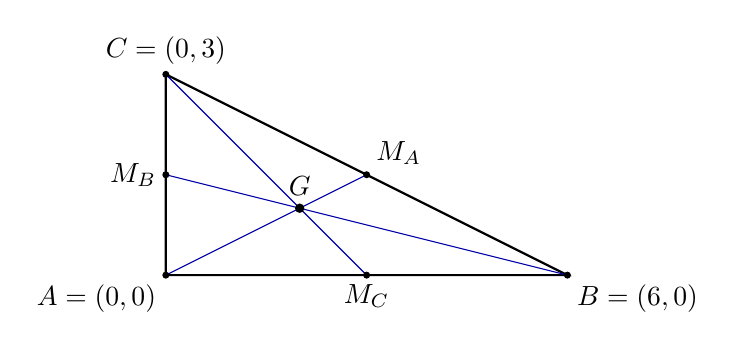
\begin{tikzpicture}[scale=.85]
 \coordinate (A) at (0,0); \coordinate (B) at (6,0);
 \coordinate (C) at (0,3); \coordinate (MA) at (3,1.5);
 \coordinate (MB) at (0,1.5); \coordinate (MC) at (3,0);
 \coordinate (G) at (2,1);
 \draw[thick] (A)--(B)--(C)--cycle;
 \draw[blue!65!black] (A)--(MA) (B)--(MB) (C)--(MC);
 \fill (G) circle (2pt) node[above=1pt] {$G$};
 \fill (A) circle (1.5pt) node[below left] {$A=(0,0)$};
 \fill (B) circle (1.5pt) node[below right] {$B=(6,0)$};
 \fill (C) circle (1.5pt) node[above] {$C=(0,3)$};
 \fill (MA) circle (1.5pt) node[above right] {$M_A$};
 \fill (MB) circle (1.5pt) node[left] {$M_B$};
 \fill (MC) circle (1.5pt) node[below] {$M_C$};
\end{tikzpicture}
\end{center}


\Needspace{5\baselineskip}
\par\bigskip
\noindent\textbf{1.7.10}\quad Prove the law of cosines starting from
$A^{2}=(\mathbf{B}-\mathbf{C})^{2}$.
\solution
Here $(\mathbf B-\mathbf C)^2$ means
$(\mathbf B-\mathbf C)\cdot(\mathbf B-\mathbf C)=|\mathbf B-\mathbf C|^2$,
and $A,B,C$ denote the side lengths $|\mathbf A|,|\mathbf B|,|\mathbf C|$.
Place the tails of $\mathbf B$ and $\mathbf C$ at the same triangle
vertex, and let $\theta$ be the included angle. The opposite side is
$\mathbf A=\mathbf B-\mathbf C$ up to orientation. Therefore
\[
 \begin{aligned}
 A^2&=(\mathbf B-\mathbf C)\cdot(\mathbf B-\mathbf C)
 =\mathbf B\cdot\mathbf B-\mathbf B\cdot\mathbf C
  -\mathbf C\cdot\mathbf B+\mathbf C\cdot\mathbf C\\
 &=\mathbf B\cdot\mathbf B+\mathbf C\cdot\mathbf C
       -2\mathbf B\cdot\mathbf C
 =B^2+C^2-2BC\cos\theta,
 \end{aligned}
\]
using $\mathbf C\cdot\mathbf B=\mathbf B\cdot\mathbf C$ and
$\mathbf B\cdot\mathbf C=BC\cos\theta$.
This is the law of cosines, reducing to Pythagoras when $\theta=\pi/2$.


\Needspace{5\baselineskip}
\par\bigskip
\noindent\textbf{1.7.11}\quad Given the three vectors,
\[
\mathbf{P}=3\hat{\mathbf{e}}_{x}+2\hat{\mathbf{e}}_{y}-\hat{\mathbf{e}}_{z},
\]
\[
\mathbf{Q}=-6\hat{\mathbf{e}}_{x}-4\hat{\mathbf{e}}_{y}+2\hat{\mathbf{e}}_{z},
\]
\[
\mathbf{R}=\hat{\mathbf{e}}_{x}-2\hat{\mathbf{e}}_{y}-\hat{\mathbf{e}}_{z},
\]
find two that are perpendicular and two that are parallel or antiparallel.
\solution
The component vectors are $\mathbf P=(3,2,-1)$,
$\mathbf Q=(-6,-4,2)$, and $\mathbf R=(1,-2,-1)$.
First $\mathbf Q=-2\mathbf P$, so $\mathbf P$ and $\mathbf Q$
are antiparallel. Next
\[
 \mathbf P\cdot\mathbf R=3(1)+2(-2)+(-1)(-1)=3-4+1=0,
\]
so $\mathbf P$ and $\mathbf R$ are perpendicular. Also
$\mathbf Q\cdot\mathbf R=-2(\mathbf P\cdot\mathbf R)=0$,
so $\mathbf Q$ and $\mathbf R$ form a second perpendicular pair.


\Needspace{9\baselineskip}
\subsection*{1.8 Complex Numbers and Functions}

\Needspace{5\baselineskip}
\par\bigskip
\noindent\textbf{1.8.1}\quad Find the reciprocal of $x+iy$, working in polar
form but expressing the final result in Cartesian form.
\solution
For $z=x+iy\ne0$, set $r=\sqrt{x^2+y^2}$ and
$z=r(\cos\theta+i\sin\theta)=re^{i\theta}$.
The reciprocal has magnitude $1/r$ and angle $-\theta$:
\[
 \frac1z=r^{-1}e^{-i\theta}
 =\frac1r(\cos\theta-i\sin\theta)
 =\boxed{\frac{x-iy}{x^2+y^2}}.
\]
Multiplication by $x+iy$ gives $(x^2+y^2)/(x^2+y^2)=1$,
checking the result. No reciprocal exists at $x=y=0$.


\Needspace{5\baselineskip}
\par\bigskip
\noindent\textbf{1.8.2}\quad Show that complex numbers have square roots and
that the square roots are contained in the complex plane. What are the square
roots of $i$?
\solution
Write a nonzero complex number as $z=re^{i\theta}$ with $r>0$.
The two numbers $w_k=\sqrt r\,e^{i(\theta/2+k\pi)}$, $k=0,1$,
satisfy $w_k^2=re^{i\theta}e^{2\pi ik}=z$. They are opposites and
are distinct. Conversely, if $w=\rho e^{i\phi}$ satisfies $w^2=z$,
then $\rho^2=r$ and $2\phi=\theta+2\pi k$, giving precisely these
two roots. Zero has the single distinct square root zero.
For $i=e^{i\pi/2}$ this gives
\[
 \boxed{\sqrt i=\pm e^{i\pi/4}=\pm\frac{1+i}{\sqrt2}}.
\]
Squaring either value gives $(1+2i-1)/2=i$.


\Needspace{5\baselineskip}
\par\bigskip
\noindent\textbf{1.8.3}\quad \erratum{For a nonnegative integer $n$ and real $\theta$,} show that
\begin{enumerate}
\item[(a)] $\displaystyle\cos n\theta=\cos^{n}\theta-\binom{n}{2}
  \cos^{n-2}\theta\sin^{2}\theta+\binom{n}{4}\cos^{n-4}\theta\sin^{4}\theta
  -\cdots,$
\item[(b)] $\displaystyle\sin n\theta=\binom{n}{1}\cos^{n-1}\theta\sin\theta
  -\binom{n}{3}\cos^{n-3}\theta\sin^{3}\theta+\cdots.$
\end{enumerate}
\solution
For a nonnegative integer $n$, de Moivre's formula and the binomial
expansion give
\[
 \cos n\theta+i\sin n\theta
 =(\cos\theta+i\sin\theta)^n
 =\sum_{j=0}^n\binom nj\cos^{n-j}\theta\,i^j\sin^j\theta.
\]
For $j=2r$, $i^{2r}=(-1)^r$, while for $j=2r+1$,
$i^{2r+1}=i(-1)^r$. Equating real and imaginary parts therefore yields
\[
 \cos n\theta=\sum_{r=0}^{\lfloor n/2\rfloor}
 (-1)^r\binom n{2r}\cos^{n-2r}\theta\sin^{2r}\theta,
\]
\[
 \sin n\theta=\sum_{r=0}^{\lfloor(n-1)/2\rfloor}
 (-1)^r\binom n{2r+1}\cos^{n-2r-1}\theta\sin^{2r+1}\theta.
\]
These are the two requested finite expansions. For $n=0$ the second
sum is empty and gives zero.


\Needspace{5\baselineskip}
\par\bigskip
\noindent\textbf{1.8.4}\quad Prove that
\begin{enumerate}
\item[(a)] $\displaystyle\sum_{n=0}^{N-1}\cos nx=\erratum{\frac{\sin(Nx/2)}{\sin(x/2)}\cos\!\left(\frac{(N-1)x}{2}\right)}$,
\item[(b)] $\displaystyle\sum_{n=0}^{N-1}\sin nx=\erratum{\frac{\sin(Nx/2)}{\sin(x/2)}\sin\!\left(\frac{(N-1)x}{2}\right)}$.
\end{enumerate}
\erratum{Here $N$ is a positive integer and $x$ is real; at $x=2\pi m$, use the continuous limits $N$ and $0$, respectively.} These series occur in the analysis of the multiple-slit diffraction pattern.
\solution
For $e^{ix}\ne1$, sum the finite geometric progression:
\[
 \sum_{n=0}^{N-1}e^{inx}=\frac{1-e^{iNx}}{1-e^{ix}}.
\]
Using $1-e^{it}=-2i e^{it/2}\sin(t/2)$ in numerator and denominator
reduces this to
\[
 \sum_{n=0}^{N-1}e^{inx}
 =e^{i(N-1)x/2}\frac{\sin(Nx/2)}{\sin(x/2)}.
\]
For real $x$ the sine quotient is real, so taking real and imaginary
parts gives (a) and (b). At $x=2\pi m$ the displayed quotient is
$0/0$, but the original sums are $N$ and $0$; these values are also
the continuous limits of the right sides. This supplies the removable
exception to the formulas.


\Needspace{5\baselineskip}
\par\bigskip
\noindent\textbf{1.8.5}\quad Assume that the trigonometric functions and the
hyperbolic functions are defined for complex argument by the appropriate power
series. Show that
\[
\erratum{i\sin z}=\sinh iz,\quad\sin iz=i\sinh z,
\]
\[
\cos z=\cosh iz,\quad\cos iz=\cosh z.
\]
\solution
\erratum{The first identity was mistranscribed: the textbook (p.~61)
has $i\sin z=\sinh(iz)$, not $i\sin(iz)=\sinh(iz)$.}
Direct substitution into the entire power series gives
\[
 \begin{aligned}
 \sinh(iz)&=\sum_{n=0}^\infty\frac{i^{2n+1}z^{2n+1}}{(2n+1)!}
       =i\sum_{n=0}^\infty\frac{(-1)^n z^{2n+1}}{(2n+1)!}=i\sin z,\\
 \sin(iz)&=\sum_{n=0}^\infty\frac{(-1)^n i^{2n+1}z^{2n+1}}{(2n+1)!}
       =i\sum_{n=0}^\infty\frac{z^{2n+1}}{(2n+1)!}=i\sinh z,\\
 \cosh(iz)&=\sum_{n=0}^\infty\frac{i^{2n}z^{2n}}{(2n)!}=\cos z,\\
 \cos(iz)&=\sum_{n=0}^\infty\frac{(-1)^n i^{2n}z^{2n}}{(2n)!}=\cosh z.
 \end{aligned}
\]
No restriction on complex $z$ is required because all four power
series converge absolutely everywhere.


\Needspace{5\baselineskip}
\par\bigskip
\noindent\textbf{1.8.6}\quad Using the identities
\[
\cos z=\frac{e^{iz}+e^{-iz}}{2},\quad\sin z=\frac{e^{iz}-e^{-iz}}{2i},
\]
established from comparison of power series, show that
\begin{enumerate}
\item[(a)] $\sin(x+iy)=\sin x\cosh y+i\cos x\sinh y$,\\
  $\cos(x+iy)=\cos x\cosh y-i\sin x\sinh y$,
\item[(b)] $|\sin z|^{2}=\sin^{2}x+\sinh^{2}y$,\quad
  $|\cos z|^{2}=\cos^{2}x+\sinh^{2}y$.
\end{enumerate}
This demonstrates that we may have $|\sin z|$, $|\cos z|>1$ in the complex
plane.
\solution
(a) For real $x,y$, $e^{i(x+iy)}=e^{-y}(\cos x+i\sin x)$ and
$e^{-i(x+iy)}=e^y(\cos x-i\sin x)$. Substituting these in the
exponential definitions and collecting terms gives
\[
 \begin{aligned}
 \sin(x+iy)&=\sin x\frac{e^y+e^{-y}}2
       +i\cos x\frac{e^y-e^{-y}}2
       =\sin x\cosh y+i\cos x\sinh y,\\
 \cos(x+iy)&=\cos x\cosh y-i\sin x\sinh y.
 \end{aligned}
\]
(b) Add the squares of each expression's real and imaginary parts:
\[
 \begin{aligned}
 |\sin z|^2&=\sin^2x\cosh^2y+\cos^2x\sinh^2y
 =\sin^2x+(\sin^2x+\cos^2x)\sinh^2y
 =\sin^2x+\sinh^2y,\\
 |\cos z|^2&=\cos^2x\cosh^2y+\sin^2x\sinh^2y
 =\cos^2x+\sinh^2y.
 \end{aligned}
\]
Here $\cosh^2y=1+\sinh^2y$ was used. For example
$|\cos(iy)|=\cosh y>1$ for $y\ne0$.


\Needspace{5\baselineskip}
\par\bigskip
\noindent\textbf{1.8.7}\quad From the identities in Exercises 1.8.5 and 1.8.6
show that
\begin{enumerate}
\item[(a)] $\sinh(x+iy)=\sinh x\cos y+i\cosh x\sin y$,\\
  $\cosh(x+iy)=\cosh x\cos y+i\sinh x\sin y$,
\item[(b)] $|\sinh z|^{2}=\sinh^{2}x+\sin^{2}y$,\quad
  \erratum{$|\cosh z|^{2}=\cosh^{2}x-\sin^{2}y$}.
\end{enumerate}
\solution
(a) Insert $e^{x+iy}=e^x(\cos y+i\sin y)$ and
$e^{-x-iy}=e^{-x}(\cos y-i\sin y)$ in the definitions of
$\sinh$ and $\cosh$. Subtracting and adding respectively yields
\[
 \sinh(x+iy)=\sinh x\cos y+i\cosh x\sin y,
 \quad
 \cosh(x+iy)=\cosh x\cos y+i\sinh x\sin y.
\]
(b) Consequently
\[
 \begin{aligned}
 |\sinh z|^2&=\sinh^2x\cos^2y+\cosh^2x\sin^2y
             =\sinh^2x+\sin^2y,\\
 |\cosh z|^2&=\cosh^2x\cos^2y+\sinh^2x\sin^2y
             =\cosh^2x-\sin^2y.
 \end{aligned}
\]
\erratum{The last sign is minus, correcting an error also present in
the textbook (p.~61).} At $x=0,y=\pi/2$, $\cosh(i\pi/2)=0$;
the corrected right side is $1-1=0$, whereas the printed plus sign
would give $2$. This independently checks the correction.


\Needspace{5\baselineskip}
\par\bigskip
\noindent\textbf{1.8.8}\quad \erratum{Put $z=x+iy$ with real $x,y$, and exclude the poles of each side.} Show that
\begin{enumerate}
\item[(a)] $\displaystyle\tanh\frac{z}{2}=\frac{\sinh x+i\sin y}{\cosh x+\cos y}$,
\item[(b)] $\displaystyle\coth\frac{z}{2}=\frac{\sinh x-i\sin y}{\cosh x-\cos y}$.
\end{enumerate}
\solution
Let $z=x+iy$ with $x,y$ real. From the exponential definitions,
$\tanh(z/2)=(e^z-1)/(e^z+1)$. Multiply numerator and denominator
by the conjugate $e^{x-iy}+1$ to obtain
\[
 \tanh\frac z2
 =\frac{e^{2x}-1+2ie^x\sin y}{e^{2x}+1+2e^x\cos y}
 =\frac{\sinh x+i\sin y}{\cosh x+\cos y}.
\]
Likewise $\coth(z/2)=(e^z+1)/(e^z-1)$. Multiplication by
$e^{x-iy}-1$ gives
\[
 \coth\frac z2
 =\frac{e^{2x}-1-2ie^x\sin y}{e^{2x}+1-2e^x\cos y}
 =\frac{\sinh x-i\sin y}{\cosh x-\cos y}.
\]
The divisions exclude the poles: $z=(2m+1)\pi i$ for $\tanh(z/2)$
and $z=2m\pi i$ for $\coth(z/2)$, $m\in\mathbb Z$.


\Needspace{5\baselineskip}
\par\bigskip
\noindent\textbf{1.8.9}\quad By comparing series expansions, show that
$\displaystyle\tan^{-1}x=\frac{i}{2}\erratum{\operatorname{Log}}\left(\frac{1-ix}{1+ix}\right)$, \erratum{for real $x$, with the principal inverse tangent and principal logarithm}.
\solution
For $|x|<1$, subtract the logarithm series on their branches through
$\log1=0$:
\[
 \log(1-ix)-\log(1+ix)
 =-2\left(ix+\frac{(ix)^3}3+\frac{(ix)^5}5+\cdots\right)
 =-2i\left(x-\frac{x^3}3+\frac{x^5}5-\cdots\right).
\]
Multiplication by $i/2$ gives exactly the Gregory series for $\arctan x$.
For all real $x$, $(1-ix)/(1+ix)$ has unit modulus and argument
$-2\arctan x\in(-\pi,\pi)$, so the principal logarithm satisfies
\[
 \boxed{\arctan x=\frac i2\operatorname{Log}\frac{1-ix}{1+ix}}.
\]
Other logarithm branches differ by $2\pi i m$ and change the right
side by $-\pi m$, the corresponding multivalued inverse-tangent branches.
For complex $x$, branch choices and the singularities $x=\pm i$
must be retained.


\Needspace{5\baselineskip}
\par\bigskip
\noindent\textbf{1.8.10}\quad Find the Cartesian form for all values of
\begin{enumerate}
\item[(a)] $(-8)^{1/3}$,
\item[(b)] $i^{1/4}$,
\item[(c)] $e^{i\pi/4}$.
\end{enumerate}
\solution
(a) Write $-8=8e^{i(\pi+2\pi k)}$. The cube roots have magnitude
$2$ and arguments $(\pi+2\pi k)/3$, $k=0,1,2$:
\[
 \boxed{1+i\sqrt3,\quad-2,\quad1-i\sqrt3}.
\]
(b) The fourth roots of $i=e^{i(\pi/2+2\pi k)}$ have arguments
$\pi/8+k\pi/2$, $k=0,1,2,3$. Set
$A=\sqrt{2+\sqrt2}/2$ and $B=\sqrt{2-\sqrt2}/2$; half-angle
identities give $\cos(\pi/8)=A$, $\sin(\pi/8)=B$. The four Cartesian
values are
\[
 \boxed{A+iB,\quad-B+iA,\quad-A-iB,\quad B-iA}.
\]
(c) The exponential is single-valued:
$\boxed{e^{i\pi/4}=(1+i)/\sqrt2}$.
Adding $2\pi$ to its angle reproduces this same value; it does not
create additional roots. Cubing the values in (a) or taking fourth
powers in (b) returns the specified original number.


\Needspace{5\baselineskip}
\par\bigskip
\noindent\textbf{1.8.11}\quad Find the polar form for all values of
\begin{enumerate}
\item[(a)] $(1+i)^{3}$,
\item[(b)] $(-1)^{1/5}$.
\end{enumerate}
\solution
(a) Since $1+i=\sqrt2 e^{i\pi/4}$,
\[
 \boxed{(1+i)^3=2\sqrt2 e^{3\pi i/4}}.
\]
This is one value, equal to $-2+2i$ in Cartesian form. Its argument
may be written $3\pi/4+2\pi m$, but all such choices represent the
same complex number.

(b) Write $-1=e^{i(\pi+2\pi k)}$. Its fifth roots are
\[
 \boxed{e^{i(2k+1)\pi/5},\qquad k=0,1,2,3,4}.
\]
They all have unit modulus. Their arguments are $\pi/5,3\pi/5,\pi,
7\pi/5,9\pi/5$, and raising any one to the fifth power gives
$e^{i(2k+1)\pi}=-1$. Values of $k$ outside this range repeat the roots.


\Needspace{9\baselineskip}
\subsection*{1.9 Derivatives and Extrema}

\Needspace{5\baselineskip}
\par\bigskip
\noindent\textbf{1.9.1}\quad Derive the following formula for the Maclaurin
expansion of a function of two variables \erratum{analytic near $(0,0)$, for $(x,y)$ within the convergence neighborhood of its Maclaurin series}:
\[
\begin{split}
f(x,y)=f(0,0)&+x\frac{\partial f}{\partial x}+y\frac{\partial f}{\partial y}\\
+\frac{1}{2!}\biggl[\binom{2}{0}x^{2}\frac{\partial^{2}f}{\partial x^{2}}
&+\binom{2}{1}xy\frac{\partial^{2}f}{\partial x\,\partial y}
+\binom{2}{2}y^{2}\frac{\partial^{2}f}{\partial y^{2}}\biggr]\\
+\frac{1}{3!}\biggl[\binom{3}{0}x^{3}\frac{\partial^{3}f}{\partial x^{3}}
&+\binom{3}{1}x^{2}y\frac{\partial^{3}f}{\partial x^{2}\,\partial y}
+\binom{3}{2}xy^{2}\frac{\partial^{3}f}{\partial x\,\partial y^{2}}
+\binom{3}{3}y^{3}\frac{\partial^{3}f}{\partial y^{3}}\biggr]+\cdots,
\end{split}
\]
where all the partial derivatives are to be evaluated at the point $(0,0)$.
\solution
\erratum{An infinite Taylor expansion represents the function only
where its remainder tends to zero; analyticity near the origin is a
sufficient hypothesis. Smoothness alone is not sufficient.}
Fix $x,y$ and define the one-variable function $F(t)=f(tx,ty)$.
The chain rule gives $F'(t)=(x\partial_x+y\partial_y)f(tx,ty)$.
Iterating, using commutation of the mixed partial derivatives, yields
\[
 F^{(n)}(0)=\sum_{j=0}^n\binom nj x^{n-j}y^j
          \frac{\partial^n f}{\partial x^{n-j}\partial y^j}(0,0).
\]
Taylor-expand $F$ about $t=0$ and then set $t=1$:
\[
 f(x,y)=\sum_{n=0}^\infty\sum_{j=0}^n
 \frac{x^{n-j}y^j}{(n-j)!j!}
 \frac{\partial^n f}{\partial x^{n-j}\partial y^j}(0,0).
\]
For $n=1$ this is $xf_x+yf_y$; for $n=2$ it is
$(x^2f_{xx}+2xyf_{xy}+y^2f_{yy})/2!$; for $n=3$ it is
$(x^3f_{xxx}+3x^2yf_{xxy}+3xy^2f_{xyy}+y^3f_{yyy})/3!$.
These are exactly the displayed terms. For a finite order $N$, ordinary
Taylor's theorem also provides a remainder $F^{(N+1)}(\theta)/(N+1)!$
for some $0<\theta<1$, under its usual real-variable hypotheses.


\Needspace{5\baselineskip}
\par\bigskip
\noindent\textbf{1.9.2}\quad The result in Exercise 1.9.1 can be generalized
to larger numbers of independent variables. Prove that for an $m$-variable
system \erratum{analytic near the origin, at points sufficiently close to it}, the Maclaurin expansion can be written in the symbolic form
\[
f(x_{1},\ldots,x_{m})
=\sum_{n=0}^{\infty}\frac{t^{n}}{n!}
\erratum{\left[\left(\sum_{i=1}^{m}\alpha_{i}
\frac{\partial}{\partial x_{i}}\right)^{n}f(\mathbf x)\right]_{\mathbf x=0}},
\]
where in the right-hand side we have made the substitutions $x_{j}=\alpha_{j}t$.
\solution
Define $F(t)=f(\alpha_1t,\ldots,\alpha_mt)$ with fixed $\alpha_i$.
The chain rule and induction give
\[
 F^{(n)}(t)=\left(\sum_{i=1}^m\alpha_i\partial_{x_i}\right)^n
 f(\alpha_1t,\ldots,\alpha_mt).
\]
Therefore Taylor's formula in $t$ is
\[
 F(t)=\sum_{n=0}^\infty\frac{t^n}{n!}
 \left[\left(\sum_{i=1}^m\alpha_i\partial_{x_i}\right)^n
 f(\mathbf x)\right]_{\mathbf x=0}.
\]
\erratum{The book's symbolic $D^nf(0)$ means that derivatives act on $f$ before evaluation at zero; the brackets in the corrected statement make this order explicit. Differentiating the constant $f(0)$ would instead give zero for $n>0$.} Since $x_i=\alpha_it$, this is the required symbolic
form. Explicitly the multinomial theorem gives
\[
 f(\mathbf x)=\sum_{r_1,\ldots,r_m\ge0}
 \frac{x_1^{r_1}\cdots x_m^{r_m}}{r_1!\cdots r_m!}
 (\partial_{x_1}^{r_1}\cdots\partial_{x_m}^{r_m}f)(0).
\]
\erratum{As in Exercise 1.9.1, equality to the infinite expansion
requires convergence to $f$; assume analyticity on the neighborhood
under consideration, or retain a finite Taylor remainder.}


\Needspace{9\baselineskip}
\subsection*{1.10 Evaluation of Integrals}

\Needspace{5\baselineskip}
\par\bigskip
\noindent\textbf{1.10.1}\quad Use a recursive method to show that, for all
positive integers $n$, $\Gamma(n)=(n-1)!$.

Evaluate the integrals in Exercises 1.10.2 through 1.10.9.
\solution
Start from $\Gamma(n)=\int_0^\infty t^{n-1}e^{-t}dt$ for $n>0$.
For an integer $n\ge1$, integration by parts gives
\[
 \Gamma(n+1)=\int_0^\infty t^n e^{-t}dt
 =[-t^n e^{-t}]_0^\infty+n\int_0^\infty t^{n-1}e^{-t}dt
 =n\Gamma(n).
\]
The boundary term vanishes because the exponential dominates any fixed
power at infinity and $t^n\to0$ at zero. The initial value is
$\Gamma(1)=\int_0^\infty e^{-t}dt=1$. Repeated application of the
recurrence yields $\Gamma(n)=(n-1)(n-2)\cdots1\,\Gamma(1)
=\boxed{(n-1)!}$, including $n=1$ with $0!=1$.


\Needspace{5\baselineskip}
\par\bigskip
\noindent\textbf{1.10.2}\quad $\displaystyle\int_{0}^{\infty}\frac{\sin x}{x}\,dx$.

\emph{Hint.}~Multiply integrand by $e^{-ax}$ and take the limit $\erratum{a\downarrow0}$.
\solution
For $a>0$ define $I(a)=\int_0^\infty e^{-ax}\sin x\,dx/x$.
Exponential decay permits differentiation under the integral:
\[
 I'(a)=-\int_0^\infty e^{-ax}\sin x\,dx
       =-\operatorname{Im}\frac1{a-i}=-\frac1{1+a^2}.
\]
Also $|I(a)|\le\int_0^\infty e^{-ax}dx=1/a$, so $I(a)\to0$
as $a\to\infty$. Integrating this derivative from $a$ to infinity gives
\[
 I(a)=\int_a^\infty\frac{dt}{1+t^2}=\frac\pi2-\arctan a.
\]
It remains to justify removing the damping. For $a\ge0$ the decreasing
function $g(x)=e^{-ax}/x$ satisfies $g'\le0$. On $[R,T]$,
\[
 \int_R^T g(x)\sin x\,dx=[-g(x)\cos x]_R^T+
                              \int_R^T g'(x)\cos x\,dx.
\]
Its absolute value is at most
$g(R)+g(T)+\int_R^T|g'(x)|dx
=g(R)+g(T)+g(R)-g(T)=2g(R)\le2/R$.
Taking $T\to\infty$ proves the same bound for the tail.
This tail bound is uniform in $a$, and the integral on $[0,R]$ tends
to its undamped value by dominated convergence. Thus the ordinary
improper integral equals $\lim_{a\downarrow0}I(a)$:
\[
 \boxed{\int_0^\infty\frac{\sin x}{x}dx=\frac\pi2}.
\]
The tail argument also proves convergence, rather than merely assigning
an Abel-summed value to the expression.


\Needspace{5\baselineskip}
\par\bigskip
\noindent\textbf{1.10.3}\quad $\displaystyle\int_{0}^{\infty}\frac{dx}{\cosh x}$.

\emph{Hint.}~\erratum{Expand the integrand using $e^{-x}$ for $x>0$, and control the integrated remainder at $x=0$.}
\solution
For $x>0$,
\[
 \frac1{\cosh x}=\frac{2e^{-x}}{1+e^{-2x}}
 =2\sum_{n=0}^N(-1)^ne^{-(2n+1)x}
  +\frac{2(-1)^{N+1}e^{-(2N+3)x}}{1+e^{-2x}}.
\]
The integral of the last term has absolute value at most $2/(2N+3)$,
so integrating and taking the limit is justified even though the
geometric series itself does not converge at $x=0$. \erratum{Thus the original hint's claim of series convergence at every relevant $x$ needs this endpoint qualification.} Therefore
\[
 \int_0^\infty\frac{dx}{\cosh x}
 =2\sum_{n=0}^\infty\frac{(-1)^n}{2n+1}=\boxed{\frac\pi2}.
\]
An independent substitution $t=e^{-x}$ gives
$2\int_0^1dt/(1+t^2)=2[\arctan t]_0^1=\pi/2$.


\Needspace{5\baselineskip}
\par\bigskip
\noindent\textbf{1.10.4}\quad
$\displaystyle\int_{0}^{\infty}\frac{dx}{e^{ax}+1}$, for $a>0$.
\solution
Set $u=e^{-ax}$ for $a>0$. Then $dx=-du/(au)$,
$e^{ax}=1/u$, and the limits $x=0,\infty$ become $u=1,0$.
Consequently
\[
 \int_0^\infty\frac{dx}{e^{ax}+1}
 =\frac1a\int_0^1\frac{du}{1+u}
 =\boxed{\frac{\ln2}{a}}.
\]
As a series check, for $x>0$ the integrand is
$e^{-ax}-e^{-2ax}+e^{-3ax}-\cdots$; integrating its finite geometric
remainder gives an error at most $1/[a(N+1)]$. Hence its integral is
$(1/a)\sum_{n\ge1}(-1)^{n-1}/n=(\ln2)/a$ as well.


\Needspace{5\baselineskip}
\par\bigskip
\noindent\textbf{1.10.5}\quad
$\displaystyle\int_{\pi}^{\infty}\frac{\sin x}{x^{2}}\,dx$.
\solution
Differentiate $\sin x/x$ to obtain
$\sin x/x^2=\cos x/x-d(\sin x/x)/dx$. On a finite interval $[\pi,R]$,
\[
 \int_\pi^R\frac{\sin x}{x^2}dx
 =\int_\pi^R\frac{\cos x}{x}dx-\left[\frac{\sin x}{x}\right]_\pi^R.
\]
The boundary term tends to zero because $\sin\pi=0$ and
$|\sin R/R|\le1/R$. With the convention
$\operatorname{Ci}(z)=-\int_z^\infty\cos t\,dt/t$ for $z>0$,
\[
 \boxed{\int_\pi^\infty\frac{\sin x}{x^2}dx
 =-\operatorname{Ci}(\pi)=-0.0736679120464255\ldots}.
\]
The negative sign is consistent with the negative first lobe on
$(\pi,2\pi)$ and the decreasing weights of subsequent lobes.
The verification script checks the result by oscillatory quadrature.


\Needspace{5\baselineskip}
\par\bigskip
\noindent\textbf{1.10.6}\quad
$\displaystyle\int_{0}^{\infty}\frac{e^{-x}\sin x}{x}\,dx$.
\solution
Use $I(a)$ derived in Exercise 1.10.2:
\[
 I(a)=\int_0^\infty\frac{e^{-ax}\sin x}{x}dx
     =\frac\pi2-\arctan a\quad(a>0).
\]
At $a=1$, this gives $\boxed{I(1)=\pi/4}$.
For a direct check, write $\sin x/x=\int_0^1\cos(tx)dt$;
absolute integrability of the exponentially damped double integral
permits interchanging integrals, giving
\[
 \int_0^1dt\int_0^\infty e^{-x}\cos(tx)dx
 =\int_0^1\frac{dt}{1+t^2}=\frac\pi4.
\]


\Needspace{5\baselineskip}
\par\bigskip
\noindent\textbf{1.10.7}\quad $\displaystyle\int_{0}^{x}\mathrm{erf}(t)\,dt$.

The result can be expressed in terms of special functions in Table 1.2.
\solution
From the definition of the error function,
$\operatorname{erf}'(t)=2e^{-t^2}/\sqrt\pi$. Integration by parts gives
\[
 \begin{aligned}
 \int_0^x\operatorname{erf}(t)dt
 &=[t\operatorname{erf}(t)]_0^x
   -\frac2{\sqrt\pi}\int_0^x t e^{-t^2}dt\\
 &=\boxed{x\operatorname{erf}(x)+\frac{e^{-x^2}-1}{\sqrt\pi}}.
 \end{aligned}
\]
Differentiating the answer cancels $2xe^{-x^2}/\sqrt\pi$ against
$-2xe^{-x^2}/\sqrt\pi$, leaving $\operatorname{erf}(x)$;
at $x=0$ the answer is zero. Both checks fix the additive constant.


\Needspace{5\baselineskip}
\par\bigskip
\noindent\textbf{1.10.8}\quad $\displaystyle\int_{1}^{x}E_{1}(t)\,dt$.

Obtain a result in which the only special function is $E_{1}$, \erratum{for real $x>0$}.
\solution
For $t>0$, $E_1(t)=\int_t^\infty e^{-u}du/u$ and hence
$E_1'(t)=-e^{-t}/t$. Integration by parts now gives
\[
 \begin{aligned}
 \int_1^x E_1(t)dt
 &=[tE_1(t)]_1^x-\int_1^x tE_1'(t)dt\\
 &=xE_1(x)-E_1(1)+\int_1^x e^{-t}dt\\
 &=\boxed{xE_1(x)-e^{-x}-E_1(1)+e^{-1}},\qquad x>0.
 \end{aligned}
\]
Its derivative is $E_1(x)+x(-e^{-x}/x)+e^{-x}=E_1(x)$,
and its value at $x=1$ is zero. Thus it has both the correct derivative
and the prescribed lower-limit constant.


\Needspace{5\baselineskip}
\par\bigskip
\noindent\textbf{1.10.9}\quad
$\displaystyle\int_{0}^{\infty}\frac{e^{-x}}{x+1}\,dx$.
\solution
Set $u=x+1$, so $e^{-x}=e\,e^{-u}$ and $dx=du$. The limits are
$u=1$ and $u=\infty$, and therefore
\[
 \int_0^\infty\frac{e^{-x}}{x+1}dx
 =e\int_1^\infty\frac{e^{-u}}u du
 =\boxed{eE_1(1)=0.596347362323194\ldots}.
\]
The integral is convergent because its integrand is bounded at zero
and bounded above by $e^{-x}$ for $x\ge0$. Direct positive-integrand
quadrature in the supplementary script checks the numerical value.


\Needspace{5\baselineskip}
\par\bigskip
\noindent\textbf{1.10.10}\quad Show that
$\displaystyle\int_{0}^{\infty}\left(\frac{\tan^{-1}x}{x}\right)^{2}dx
=\pi\ln2$.

\emph{Hint.}~Integrate by parts, to linearize in $\tan^{-1}$. Then replace
$\tan^{-1}x$ by $\tan^{-1}ax$ and evaluate for $a=1$.
\solution
Integrate by parts with $u=(\arctan x)^2$ and $dv=dx/x^2$:
\[
 I=\left[-\frac{(\arctan x)^2}{x}\right]_0^\infty
       +2\int_0^\infty\frac{\arctan x}{x(1+x^2)}dx.
\]
The boundary term vanishes: near zero its magnitude is $O(x)$, and
at infinity it is $O(1/x)$. Define, for $a\ge0$,
\[
 J(a)=2\int_0^\infty\frac{\arctan(ax)}{x(1+x^2)}dx,
 \qquad I=J(1),\qquad J(0)=0.
\]
Differentiation is dominated by $2/(1+x^2)$ and yields
\[
 J'(a)=2\int_0^\infty\frac{dx}{(1+x^2)(1+a^2x^2)}.
\]
For $a>0$, $a\ne1$, partial fractions give
\[
 \frac1{(1+x^2)(1+a^2x^2)}
 =\frac1{1-a^2}\left(\frac1{1+x^2}-\frac{a^2}{1+a^2x^2}\right),
\]
so $J'(a)=2(\pi/2-a\pi/2)/(1-a^2)=\pi/(1+a)$.
Continuity of the integral extends this to $a=0,1$.
Integrating from $0$ to $a$ gives $J(a)=\pi\ln(1+a)$, and hence
$\boxed{I=\pi\ln2}$.


\Needspace{5\baselineskip}
\par\bigskip
\noindent\textbf{1.10.11}\quad By direct integration in Cartesian coordinates,
find the area of the ellipse with \erratum{positive semiaxes $a,b$}, defined by
\[
\frac{x^{2}}{a^{2}}+\frac{y^{2}}{b^{2}}=1.
\]
\solution
Take $a,b>0$. In the first quadrant the ellipse has upper boundary
$y=b\sqrt{1-x^2/a^2}$, $0\le x\le a$. Reflection symmetry gives
\[
 A=4b\int_0^a\sqrt{1-x^2/a^2}\,dx.
\]
Use $x=a\sin\theta$, $dx=a\cos\theta\,d\theta$, with
$0\le\theta\le\pi/2$:
\[
 A=4ab\int_0^{\pi/2}\cos^2\theta\,d\theta
  =2ab\left[\theta+\frac12\sin2\theta\right]_0^{\pi/2}
  =\boxed{\pi ab}.
\]
For $a=b=r$ this reduces to the circle area $\pi r^2$, checking the
scale and numerical coefficient.


\Needspace{5\baselineskip}
\par\bigskip
\noindent\textbf{1.10.12}\quad A unit circle is divided into two pieces by a
straight line whose distance of closest approach to the center is $1/2$ unit.
By evaluating a suitable integral, find the area of the smaller piece thereby
produced. Then use simple geometric considerations to verify your answer.
\solution
Rotate coordinates so that the cutting line is $x=1/2$ in the unit
circle $x^2+y^2=1$. The smaller cap has vertical extent
$2\sqrt{1-x^2}$, so
\[
 \begin{aligned}
 A&=2\int_{1/2}^1\sqrt{1-x^2}\,dx\\
  &=\left[x\sqrt{1-x^2}+\arcsin x\right]_{1/2}^1
   =\frac\pi2-\left(\frac{\sqrt3}4+\frac\pi6\right)
   =\boxed{\frac\pi3-\frac{\sqrt3}4}.
 \end{aligned}
\]
For the geometric check, the chord's endpoints make angles $\pm\pi/3$
with the positive $x$ axis. The sector between them has angle $2\pi/3$
and area $(1/2)(2\pi/3)=\pi/3$. The triangle cut off from that sector
has base $\sqrt3$ and altitude $1/2$, hence area $\sqrt3/4$.
Subtracting gives the same cap area.


\Needspace{9\baselineskip}
\subsection*{1.11 Dirac Delta Function}

\Needspace{5\baselineskip}
\par\bigskip
\noindent\textbf{1.11.1}\quad Let
\[
\delta_{n}(x)=\begin{cases}
0, & x<-\dfrac{1}{2n},\\[6pt]
n, & -\dfrac{1}{2n}<x<\dfrac{1}{2n},\\[6pt]
0, & \dfrac{1}{2n}<x.
\end{cases}
\]
Show that
\[
\lim_{n\to\infty}\int_{-\infty}^{\infty}f(x)\delta_{n}(x)\,dx=f(0),
\]
assuming that $f(x)$ is \erratum{locally integrable and} continuous at $x=0$.
\solution
The rectangle has width $1/n$ and height $n$, so its integral is $1$.
Subtracting $f(0)$ under the integral gives the useful explicit bound
\[
 \begin{aligned}
 \left|\int_{\mathbb R}f(x)\delta_n(x)dx-f(0)\right|
 &=\left|n\int_{-1/(2n)}^{1/(2n)}[f(x)-f(0)]dx\right|\\
 &\le\sup_{|x|\le1/(2n)}|f(x)-f(0)|.
 \end{aligned}
\]
Continuity at zero makes the supremum tend to zero: for each
$\epsilon>0$, take $\eta>0$ with $|f(x)-f(0)|<\epsilon$ when
$|x|<\eta$, then take $n>1/(2\eta)$. This proves the desired limit.
The unspecified values at the two endpoints do not affect an integral.


\Needspace{5\baselineskip}
\par\bigskip
\noindent\textbf{1.11.2}\quad For
\[
\delta_{n}(x)=\frac{n}{\pi}\,\frac{1}{1+n^{2}x^{2}},
\]
show that
\[
\int_{-\infty}^{\infty}\delta_{n}(x)\,dx=1.
\]
\solution
For $n>0$ use $u=nx$, so $dx=du/n$. Then
\[
 \int_{-\infty}^\infty\delta_n(x)dx
 =\frac1\pi\int_{-\infty}^\infty\frac{du}{1+u^2}
 =\frac1\pi[\arctan u]_{-\infty}^\infty
 =\frac1\pi\left(\frac\pi2+\frac\pi2\right)=1.
\]
This proves normalization for each $n$, not merely in the limit.
It also displays why the numerator must contain the factor $n$.


\Needspace{5\baselineskip}
\par\bigskip
\noindent\textbf{1.11.3}\quad Fejer's method of summing series is associated
with the function
\[
\delta_{n}(t)=\frac{1}{2\pi n}\left[\frac{\sin(nt/2)}{\sin(t/2)}\right]^{2}.
\]
Show that $\delta_{n}(t)$ is a delta distribution \erratum{on one period, for continuous $f$,} in the sense that
\[
\lim_{n\to\infty}\frac{1}{2\pi n}\erratum{\int_{-\pi}^{\pi}}f(t)
\left[\frac{\sin(nt/2)}{\sin(t/2)}\right]^{2}dt=f(0).
\]
\solution
\erratum{The printed whole-line assertion is false. On one period,
$\int_{-\pi}^{\pi} f(t)\delta_n(t)dt\to f(0)$ for continuous $f$.
On the whole real line the distributional limit is instead the comb
$\sum_{m\in\mathbb Z}\delta(t-2\pi m)$.}
For integer $n\ge1$, the finite geometric sum gives
\[
 \delta_n(t)=\frac1{2\pi n}\left|\sum_{j=0}^{n-1}e^{ijt}\right|^2
 =\frac1{2\pi}\sum_{k=-(n-1)}^{n-1}
                  \left(1-\frac{|k|}{n}\right)e^{ikt}.
\]
The modulus-square expression proves positivity; integrating the finite
Fourier sum over $[-\pi,\pi]$ leaves only its constant term, giving
$\int_{-\pi}^{\pi}\delta_n(t)dt=1$.
For any $0<\eta<\pi$, if $\eta\le|t|\le\pi$ then
\[
 0\le\delta_n(t)\le\frac1{2\pi n\sin^2(\eta/2)},\qquad
 \int_{\eta\le|t|\le\pi}\delta_n(t)dt
       \le\frac1{n\sin^2(\eta/2)}\to0.
\]
Subtract $f(0)$ and split the integral into $|t|<\eta$ and its
complement. The first part is at most
$\sup_{|t|<\eta}|f(t)-f(0)|$, which continuity makes arbitrarily small.
For bounded continuous $f$ the second is at most
$2\|f\|_\infty/[n\sin^2(\eta/2)]\to0$. This proves the one-period result.
For a smooth compactly supported test function on the whole line,
partition its support into periods and use $2\pi$-periodicity of
$\delta_n$. The same argument gives
\[
 \lim_{n\to\infty}\int_{\mathbb R} f(t)\delta_n(t)dt
       =\sum_{m\in\mathbb Z} f(2\pi m).
\]
Only finitely many terms occur for such a test function. Choosing it
supported near $2\pi$, with $f(2\pi)=1$ and $f(0)=0$, directly
contradicts the original claim and verifies the correction.


\Needspace{5\baselineskip}
\par\bigskip
\noindent\textbf{1.11.4}\quad Prove that
\[
\delta[a(x-x_{1})]=\erratum{\frac{1}{|a|}}\,\delta(x-x_{1}),\qquad \erratum{a\ne0}.
\]
\emph{Note.}~\erratum{The absolute value is required for all real nonzero $a$, including negative $a$.}
\solution
\erratum{For every real $a\ne0$ the factor is $1/|a|$; evenness is
not an optional extra convention for the Dirac distribution.}
Test the identity against a smooth compactly supported $\phi$ and
make the change of variable $u=a(x-x_1)$. The orientation of the
integration limits changes when $a<0$, producing the absolute Jacobian:
\[
 \int_{\mathbb R}\phi(x)\delta(a(x-x_1))dx
 =\frac1{|a|}\int_{\mathbb R}\phi(x_1+u/a)\delta(u)du
 =\frac{\phi(x_1)}{|a|}.
\]
This equals the action of $\delta(x-x_1)/|a|$, proving the distribution
identity. For $a>0$ it reduces to the printed factor $1/a$.
The value $a=0$ is excluded because $\delta(0)$ is not a distribution
obtained by this change of variable.


\Needspace{5\baselineskip}
\par\bigskip
\noindent\textbf{1.11.5}\quad \erratum{For distinct real $x_1,x_2$,} show that
\[
\delta[(x-x_{1})(x-x_{2})]
=[\delta(x-x_{1})+\delta(x-x_{2})]/|x_{1}-x_{2}|.
\]
\emph{Hint.}~Try using Exercise 1.11.4.
\solution
\erratum{Assume distinct real roots $x_1\ne x_2$.}
Let $g(x)=(x-x_1)(x-x_2)$. Near either simple root, use the local
variable $u=g(x)$, with $dx=du/|g'(x)|$ in a real integral.
Since
\[
 g'(x)=2x-x_1-x_2,\quad
 g'(x_1)=x_1-x_2,\quad g'(x_2)=x_2-x_1,
\]
a test function $\phi$ has integral
\[
 \int_{\mathbb R}\phi(x)\delta(g(x))dx
 =\frac{\phi(x_1)}{|x_1-x_2|}+\frac{\phi(x_2)}{|x_2-x_1|}.
\]
There is no contribution away from the roots, where $g$ stays away
from zero locally. Recognizing the two evaluation functionals proves
\[
 \delta((x-x_1)(x-x_2))
 =\frac{\delta(x-x_1)+\delta(x-x_2)}{|x_1-x_2|}.
\]
For coincident roots the Jacobian vanishes and this formula does not
apply; its singular denominator cannot simply be assigned a value.


\Needspace{5\baselineskip}
\par\bigskip
\noindent\textbf{1.11.6}\quad Using the Gauss error curve delta sequence
$\delta_{n}=\dfrac{n}{\sqrt{\pi}}e^{-n^{2}x^{2}}$, show that
\[
\erratum{x\frac{d}{dx}\delta(x)}=-\delta(x),
\]
treating $\delta(x)$ and its derivative as in Eq.~(1.157).
\solution
\erratum{The textbook (p.~81) asks for $x\delta'(x)=-\delta(x)$.
The transcribed derivative of the product is incorrect:
$(x\delta(x))'=0$, since $x\delta(x)=0$.}
For the specified Gaussian sequence,
\[
 \delta_n'(x)=-\frac{2n^3x}{\sqrt\pi}e^{-n^2x^2}.
\]
Against a smooth compactly supported test function $\phi$, substitute
$y=nx$ to obtain
\[
 \int_{\mathbb R}x\delta_n'(x)\phi(x)dx
 =-\frac2{\sqrt\pi}\int_{\mathbb R}y^2e^{-y^2}\phi(y/n)dy.
\]
Dominated convergence is justified by the integrable bound
$\|\phi\|_\infty y^2e^{-y^2}$. Integration by parts gives
\[
 \int_{\mathbb R}y^2e^{-y^2}dy
 =-\frac12[y e^{-y^2}]_{-\infty}^\infty
       +\frac12\int_{\mathbb R}e^{-y^2}dy=\frac{\sqrt\pi}{2}.
\]
Hence the limit is $-\phi(0)$, exactly the action of $-\delta$.
This proves $x\delta'=-\delta$. The product rule then gives
$(x\delta)'=\delta+x\delta'=0$, an independent consistency check.


\Needspace{5\baselineskip}
\par\bigskip
\noindent\textbf{1.11.7}\quad Show that
\[
\int_{-\infty}^{\infty}\delta'(x)f(x)\,dx=-f'(0).
\]
Here we assume that $f'(x)$ is continuous at $x=0$.
\solution
A distributional derivative is defined by its action on test functions,
$\langle T',f\rangle=-\langle T,f'\rangle$. Taking $T=\delta$ gives
\[
 \boxed{\int_{\mathbb R}\delta'(x)f(x)dx=-f'(0)}.
\]
To check this from regular functions, use a smooth delta sequence
$\delta_n$ and a smooth compactly supported $f$. Ordinary integration
by parts gives
\[
 \int_{\mathbb R}\delta_n'(x)f(x)dx
 =[\delta_n(x)f(x)]_{-\infty}^\infty
    -\int_{\mathbb R}\delta_n(x)f'(x)dx
 =-\int_{\mathbb R}\delta_n(x)f'(x)dx.
\]
The boundary term vanishes by compact support. Continuity of $f'$ at
zero then makes the last integral tend to $-f'(0)$, reproducing the
distributional definition and fixing the minus sign.
Only the values near zero matter: multiply any locally $C^1$ function
by a smooth cutoff equal to $1$ there. Since $\delta'$ is supported
at zero, this leaves its action unchanged. The identity therefore
extends to the local regularity stated in the question without imposing
any behavior on $f$ at infinity.


\Needspace{5\baselineskip}
\par\bigskip
\noindent\textbf{1.11.8}\quad Prove that
\[
\delta(f(x))=\erratum{\frac{1}{|f\prime(x_0)|}}\delta(x-x_{0}),
\]
where \erratum{$f$ is real and $C^1$, and $x_0$ is its unique simple real zero, so $f(x_0)=0$ and $f\prime(x_0)\ne0$}.

\emph{Hint.}~\erratum{Use the local variable $u=f(x)$ and the absolute Jacobian $1/|f\prime(x_0)|$ at each simple zero.}
\solution
\erratum{For a unique simple real zero $x_0$, the factor must be
$1/|f'(x_0)|$. For multiple simple zeros, add their contributions.}
Let $f$ be a real $C^1$ function on the domain under consideration,
with $f'(x_i)\ne0$ at every zero $x_i$. The inverse function theorem supplies a local
inverse $x=x_i(u)$ for $u=f(x)$. Restricting a test function $\phi$
to this neighborhood and changing variables gives
\[
 \int\phi(x)\delta(f(x))dx
 =\int\frac{\phi(x_i(u))}{|f'(x_i(u))|}\delta(u)du
 =\frac{\phi(x_i)}{|f'(x_i)|}.
\]
A partition into neighborhoods of the zeros (only finitely many in a
compact test support) therefore yields
\[
 \boxed{\delta(f(x))=\sum_{i:f(x_i)=0}
                  \frac{\delta(x-x_i)}{|f'(x_i)|}}.
\]
The printed single-root formula is recovered only with the additional
positive-derivative assumption. A negative derivative reverses limits,
which is why the absolute value is necessary. A repeated zero has
$f'(x_i)=0$ and lies outside this formula's hypotheses.


\Needspace{5\baselineskip}
\par\bigskip
\noindent\textbf{1.11.9}\quad
\begin{enumerate}
\item[(a)] If we define a sequence $\delta_{n}(x)=n/(2\cosh^{2}nx)$, show that
  \[
  \int_{-\infty}^{\infty}\delta_{n}(x)\,dx=1,\quad\text{independent of }n.
  \]
\item[(b)] Continuing this analysis, show that\footnote{Many other symbols are
  used for this function. This is the AMS-55 notation (in Additional Readings,
  see Abramowitz and Stegun): $u$ for unit.}
  \[
  \int_{-\infty}^{x}\erratum{\delta_{n}(t)\,dt}=\frac{1}{2}[1+\tanh nx]\equiv u_{n}(x)
  \]
  and
  \[
  \lim_{n\to\infty}u_{n}(x)=\begin{cases}0,&x<0,\\1,&x>0.\end{cases}
  \]
  This is the Heaviside unit step function (Fig.~1.23).
\end{enumerate}
\solution
(a) For $n>0$, substitute $u=nx$:
\[
 \int_{-\infty}^\infty\frac{n}{2\cosh^2(nx)}dx
 =\frac12\int_{-\infty}^\infty\operatorname{sech}^2u\,du
 =\frac12[\tanh u]_{-\infty}^\infty=1.
\]
(b) \erratum{Use a separate dummy variable in the integral.} Since
$d(\tanh nt)/dt=n\operatorname{sech}^2(nt)$,
\[
 u_n(x)=\int_{-\infty}^x\delta_n(t)dt
       =\frac12[\tanh(nt)]_{t=-\infty}^{t=x}
       =\frac12[1+\tanh(nx)].
\]
If $x>0$, $nx\to+\infty$ and $u_n(x)\to1$; if $x<0$,
$nx\to-\infty$ and $u_n(x)\to0$. At $x=0$ every $u_n(0)=1/2$,
so this symmetric sequence selects the convention $u(0)=1/2$.
The value at a single point does not affect its distributional derivative,
which is $\delta$.
